%%%%%%%%%%%%%%%%%%%%%%%%%%%%%%%%%%%%%%%%%%%%%%%%%%%%%%%%%%%%%%%%%%%%%%%%%%%%%%%
%                       CARREGA DE LA CLASSE DE DOCUMENT                      %
%                                                                             %
% Les opcions admissibles son:                                                %
%      12pt / 11pt            (cos dels tipus de lletra; no feu servir 10pt)  %
%                                                                             %
% catalan/spanish/english     (llengua principal del treball)                 %
%                                                                             % 
% french/italian/german...    (si necessiteu fer servir alguna altra llengua) %
%                                                                             %
% listoffigures               (El document inclou un Index de figures)        %
% listoftables                (El document inclou un Index de taules)         %
% listofquadres               (El document inclou un Index de quadres)        %
% listofalgorithms            (El document inclou un Index d'algorismes)      %
%                                                                             %
%%%%%%%%%%%%%%%%%%%%%%%%%%%%%%%%%%%%%%%%%%%%%%%%%%%%%%%%%%%%%%%%%%%%%%%%%%%%%%%

\documentclass[11pt,oneside,spanish,listoffigures,listoftables]{tfgetsinf}

%%%%%%%%%%%%%%%%%%%%%%%%%%%%%%%%%%%%%%%%%%%%%%%%%%%%%%%%%%%%%%%%%%%%%%%%%%%%%%%
%                     CODIFICACIO DEL FITXER FONT                             %
%                                                                             %
%    windows fa servir normalment 'ansinew'                                   %
%    amb linux es possible que siga 'latin1' o 'latin9'                       %
%    Pero el mes recomanable es fer servir utf8 (unicode 8)                   %
%                                          (si el vostre editor ho permet)    % 
%%%%%%%%%%%%%%%%%%%%%%%%%%%%%%%%%%%%%%%%%%%%%%%%%%%%%%%%%%%%%%%%%%%%%%%%%%%%%%%

\usepackage[utf8]{inputenc} 
\usepackage{hyperref}
%%%%%%%%%%%%%%%%%%%%%%%%%%%%%%%%%%%%%%%%%%%%%%%%%%%%%%%%%%%%%%%%%%%%%
% Para conseguir que la tabla de contenido no salga en rojo
%%%%%%%%%%%%%%%%%%%%%%%%%%%%%%%%%%%%%%%%%%%%%%%%%%%%%%%%%%%%%%%%%%%%%

\hypersetup{ colorlinks=true, linkcolor=black, urlcolor=cyan, }

% Paquetes para diagramas (TikZ) y tablas
\usepackage{tikz}
\usetikzlibrary{arrows.meta, positioning, shapes.geometric, fit, shapes.multipart}
\usepackage{booktabs}
\usepackage{tabularx}
\usepackage{pgfgantt}
\usepackage{graphicx}
\usepackage{pdflscape}
\usepackage{pifont} % Simbolos de cumplimiento (checkmark / cruz) para la matriz de ODS

% Parametros de colocacion de flotantes: permiten que figuras y tablas ocupen
% mas espacio de cada pagina, reduciendo los huecos en blanco que dejan los
% flotantes altos (p. ej. los diagramas TikZ) al no poder colocarse "aqui".
\renewcommand{\topfraction}{0.9}
\renewcommand{\bottomfraction}{0.8}
\renewcommand{\textfraction}{0.07}
\renewcommand{\floatpagefraction}{0.75}
\setcounter{topnumber}{3}
\setcounter{bottomnumber}{2}
\setcounter{totalnumber}{5}

% Paquete para incluir fragmentos de código fuente
\usepackage{listings}
\lstdefinestyle{codigofuente}{
  basicstyle=\footnotesize\ttfamily,
  numbers=left,
  numberstyle=\tiny\color{gray},
  numbersep=8pt,
  breaklines=true,
  frame=single,
  framesep=4pt,
  xleftmargin=16pt,
  showstringspaces=false,
  tabsize=2,
  captionpos=b,
  aboveskip=6pt,
  belowskip=4pt
}
\lstset{style=codigofuente}

%%%%%%%%%%%%%%%%%%%%%%%%%%%%%%%%%%%%%%%%%%%%%%%%%%%%%%%%%%%%%%%%%%%%%%%%%%%%%%%
%                        ALTRES PAQUETS I DEFINICIONS                         %
%                                                                             %
% Carregueu aci els paquets que necessiteu i declareu les comandes i entorns  %
%                                          (aquesta seccio pot ser buida)     %
%%%%%%%%%%%%%%%%%%%%%%%%%%%%%%%%%%%%%%%%%%%%%%%%%%%%%%%%%%%%%%%%%%%%%%%%%%%%%%%



%%%%%%%%%%%%%%%%%%%%%%%%%%%%%%%%%%%%%%%%%%%%%%%%%%%%%%%%%%%%%%%%%%%%%%%%%%%%%%%
%                        DADES DEL TREBALL                                    %
%                                                                             %
% titol, alumne, tutor i curs academic                                        %
%%%%%%%%%%%%%%%%%%%%%%%%%%%%%%%%%%%%%%%%%%%%%%%%%%%%%%%%%%%%%%%%%%%%%%%%%%%%%%%

\title{Diseño y desarrollo de una plataforma de\\
         conectividad en una red de acción social}
\author{Saúl Alcázar López}
\tutor{José Hilario Canós Cerdá}
\curs{2025-2026}

%%%%%%%%%%%%%%%%%%%%%%%%%%%%%%%%%%%%%%%%%%%%%%%%%%%%%%%%%%%%%%%%%%%%%%%%%%%%%%%
%                     PARAULES CLAU/PALABRAS CLAVE/KEY WORDS                  %
%                                                                             %
% Independentment de la llengua del treball, s'hi han d'incloure              %
% les paraules clau i el resum en els tres idiomes                            %
%%%%%%%%%%%%%%%%%%%%%%%%%%%%%%%%%%%%%%%%%%%%%%%%%%%%%%%%%%%%%%%%%%%%%%%%%%%%%%%

\keywords{acció social, tercer sector, plataforma web, traçabilitat, donacions, aplicació full-stack} % Paraules clau
         {acción social, tercer sector, plataforma web, trazabilidad, donaciones, aplicación full-stack}              % Palabras clave
         {social action, third sector, web platform, traceability, donations, full-stack application}        % Key words

%%%%%%%%%%%%%%%%%%%%%%%%%%%%%%%%%%%%%%%%%%%%%%%%%%%%%%%%%%%%%%%%%%%%%%%%%%%%%%%
%                              INICI DEL DOCUMENT                             %
%%%%%%%%%%%%%%%%%%%%%%%%%%%%%%%%%%%%%%%%%%%%%%%%%%%%%%%%%%%%%%%%%%%%%%%%%%%%%%%

\begin{document}

%%%%%%%%%%%%%%%%%%%%%%%%%%%%%%%%%%%%%%%%%%%%%%%%%%%%%%%%%%%%%%%%%%%%%%%%%%%%%%%
%              RESUMS DEL TFG EN VALENCIA, CASTELLA I ANGLES                  %
%%%%%%%%%%%%%%%%%%%%%%%%%%%%%%%%%%%%%%%%%%%%%%%%%%%%%%%%%%%%%%%%%%%%%%%%%%%%%%%

\begin{abstract}
El propòsit d'aquest treball és el disseny i desenvolupament d'una plataforma web de suport a AskingX, un moviment d'acció social que connecta entitats del tercer sector —ONG, col·legis i persones en situació de vulnerabilitat— amb donants i experts disposats a cobrir les seues necessitats. El model s'articula al voltant de la figura del facilitador humà (\textit{AskAuthor}), que tradueix aquestes necessitats en peticions concretes i les encamina fins a trobar qui puga satisfer-les. Quan la gestió manual d'aquestes peticions esdevé inviable pel volum d'activitat, sorgeix la necessitat d'una eina que automatitze el seguiment sense substituir la mediació humana.

La solució desenvolupada és una aplicació \textit{full-stack} que gestiona el cicle de vida complet de cada petició mitjançant una màquina d'estats, controla els lliuraments parcials d'ajuda i aplica un control d'accés per rols que protegeix les dades dels col·lectius vulnerables. El servidor es construeix amb Node.js, Express i Prisma sobre una base de dades PostgreSQL, mentre que el client és una aplicació d'una sola pàgina desenvolupada amb React. S'hi integra a més un model de llenguatge per a generar, sota supervisió humana, narratives d'impacte a partir de les col·laboracions completades.

El sistema s'ha validat mitjançant proves funcionals, d'interfície i de seguretat, i s'acompanya de quadres de comandament que permeten avaluar el progrés de l'activitat. El resultat és una plataforma funcional, traçable i replicable, concebuda per a créixer i estendre's a altres ciutats de la xarxa.
\end{abstract}
\begin{abstract}[spanish]
El propósito de este trabajo es el diseño y desarrollo de una plataforma web de soporte a AskingX, un movimiento de acción social que conecta entidades del tercer sector —ONG, colegios y personas en situación de vulnerabilidad— con donantes y expertos dispuestos a cubrir sus necesidades. El modelo se articula en torno a la figura del facilitador humano (\textit{AskAuthor}), que traduce esas necesidades en peticiones concretas y las encamina hasta encontrar a quien pueda satisfacerlas. Cuando la gestión manual de estas peticiones se vuelve inviable por el volumen de actividad, surge la necesidad de una herramienta que automatice el seguimiento sin sustituir la mediación humana.

La solución desarrollada es una aplicación \textit{full-stack} que gestiona el ciclo de vida completo de cada petición mediante una máquina de estados, controla las entregas parciales de ayuda y aplica un control de acceso por roles que protege los datos de los colectivos vulnerables. El servidor se construye con Node.js, Express y Prisma sobre una base de datos PostgreSQL, mientras que el cliente es una aplicación de página única desarrollada con React. Se integra además un modelo de lenguaje para generar, bajo supervisión humana, narrativas de impacto a partir de las colaboraciones completadas.

El sistema se ha validado mediante pruebas funcionales, de interfaz y de seguridad, y se acompaña de cuadros de mando que permiten evaluar el progreso de la actividad. El resultado es una plataforma funcional, trazable y replicable, concebida para crecer y extenderse a otras ciudades de la red.
\end{abstract}
\begin{abstract}[english]
The purpose of this work is the design and development of a web platform supporting AskingX, a social-action movement that connects third-sector organisations —NGOs, schools and people in vulnerable situations— with donors and experts willing to meet their needs. The model revolves around the human facilitator (the \textit{AskAuthor}), who translates those needs into concrete requests and routes them until someone able to fulfil them is found. When handling these requests manually becomes unfeasible due to the volume of activity, a tool is needed to automate the tracking without replacing the human mediation.

The solution developed is a \textit{full-stack} application that manages the complete life cycle of each request through a state machine, controls the partial deliveries of aid and enforces role-based access control that protects the data of vulnerable groups. The server is built with Node.js, Express and Prisma on top of a PostgreSQL database, while the client is a single-page application developed with React. A large language model is also integrated to generate, under human supervision, impact narratives from the completed collaborations.

The system has been validated through functional, interface and security testing, and is complemented by dashboards that make it possible to assess the progress of the activity. The result is a functional, traceable and replicable platform, conceived to grow and expand to other cities in the network.
\end{abstract}

%%%%%%%%%%%%%%%%%%%%%%%%%%%%%%%%%%%%%%%%%%%%%%%%%%%%%%%%%%%%%%%%%%%%%%%%%%%%%%%
%                              CONTINGUT DEL TREBALL                          %
%%%%%%%%%%%%%%%%%%%%%%%%%%%%%%%%%%%%%%%%%%%%%%%%%%%%%%%%%%%%%%%%%%%%%%%%%%%%%%%

\mainmatter

%%%%%%%%%%%%%%%%%%%%%%%%%%%%%%%%%%%%%%%%%%%%%%%%%%%%%%%%%%%%%%%%%%%%%%%%%%%%%%%
%                                  INTRODUCCIO                                %
%%%%%%%%%%%%%%%%%%%%%%%%%%%%%%%%%%%%%%%%%%%%%%%%%%%%%%%%%%%%%%%%%%%%%%%%%%%%%%%

\chapter{Introducción}
\section{Motivación}
Las ciudades contemporáneas concentran una cantidad enorme de recursos, capacidades y conocimiento técnico que, sin embargo, rara vez llegan donde más se necesitan. Organizaciones del tercer sector, instituciones educativas y ciudadanos conviven en el mismo territorio pero operan de forma aislada, separados por barreras relacionales y organizativas que hacen muy costoso el simple acto de conectar a quien tiene algo que ofrecer con quien lo necesita. El problema, en definitiva, no suele ser la falta de recursos: es el coste de movilizarlos.

AskingX nace precisamente para atacar ese problema. No es una plataforma de voluntariado al uso ni un repositorio de subvenciones, sino un modelo relacional que introduce la figura del \textit{AskAuthor}: un facilitador humano encargado de escuchar a las organizaciones, traducir sus carencias en peticiones concretas (\textit{Asks}) y conectarlas con personas o entidades capaces de cubrirlas (\textit{Givers}) \cite{canos_manley_2024}. La mediación humana no es aquí un defecto del sistema, sino su característica más esencial.

La motivación de este Trabajo de Fin de Grado surge de un problema práctico muy concreto. La iniciativa, aplicada actualmente bajo el nombre de \textit{AskingValència}, ha alcanzado un volumen de actividad en el que gestionar las peticiones de forma manual resulta inviable. Hacer el seguimiento del estado de cada \textit{Ask}, controlar qué perfiles pueden acceder a qué información y documentar las entregas parciales de ayuda consume el tiempo que los facilitadores deberían dedicar a construir relaciones.

Por eso, la plataforma que se desarrolla en este trabajo no pretende reemplazar esa dimensión humana, sino liberarla de la carga operativa que la frena. El objetivo es construir una herramienta técnica —servidor y cliente web— que gestione de forma transparente el ciclo de vida de las peticiones, aplique un control de acceso estricto según el rol de cada usuario (RBAC) y proporcione a la red AskingX la base tecnológica necesaria para crecer y replicarse en otras ciudades.

\section{Objetivos}
Expuesta la motivación, conviene concretar qué se persigue exactamente con este trabajo. Las metas se han organizado en un objetivo general, que fija el propósito último del proyecto, y un conjunto de objetivos específicos de carácter técnico que articulan el camino para alcanzarlo.
\subsection{Objetivo general}
El objetivo de este trabajo es analizar el modelo organizativo de AskingX y desarrollar una plataforma tecnológica que apoye su gestión interna. La solución debe permitir documentar, gestionar y escalar el flujo de interacciones entre los actores de la red en el contexto de \textit{AskingValència}, integrando tanto la lógica de negocio del servidor como una interfaz de usuario adaptada a los distintos perfiles operativos del sistema.
\subsection{Objetivos específicos}
Para alcanzar el objetivo general, se han definido los siguientes objetivos de carácter técnico y funcional:

\begin{enumerate}
    \item \textbf{Analizar el modelo relacional de AskingX.} Comprender las dinámicas operativas y los cuatro roles del sistema (\textit{Asker}, \textit{Giver}, \textit{AskAuthor} y \textit{Connector}) para trasladar sus necesidades a un modelo de requisitos de software.

    \item \textbf{Diseñar e implementar una arquitectura cliente-servidor.} Construir una solución que desacople la capa de presentación de la lógica de negocio, estructurando el servidor en capas independientes (Rutas, Controladores y Servicios) para facilitar el mantenimiento y la evolución del sistema.

    \item \textbf{Modelar la persistencia de datos.} Diseñar y desplegar una base de datos PostgreSQL gestionada a través de Prisma ORM, que dé soporte a la trazabilidad completa de las peticiones y a las entregas parciales de ayuda.

    \item \textbf{Garantizar la seguridad y el control de acceso.} Implementar autenticación basada en el estándar JWT y una política RBAC que asegure que cada perfil opere exclusivamente dentro de sus competencias funcionales.

    \item \textbf{Desarrollar el ciclo de vida de las peticiones como una máquina de estados.} Programar la lógica de negocio para gestionar las transiciones entre estados (desde \textit{CREATED} hasta \textit{FULFILLED}), incluyendo un mecanismo de validación que controle las entregas parciales y bloquee cualquier sobredonación.

    \item \textbf{Integrar servicios de Inteligencia Artificial.} Diseñar un módulo de conexión con un modelo de lenguaje (LLM) que automatice la generación supervisada de Historias de Impacto a partir de las colaboraciones completadas con éxito.
\end{enumerate}
\section{Impacto Esperado}
La plataforma que se desarrolla en este trabajo no aspira a transformar la esencia del modelo AskingX. Lo que se busca es algo más concreto: reducir la fricción operativa que hoy limita su crecimiento. Se espera que su puesta en marcha genere un impacto positivo en cuatro ámbitos:

\begin{itemize}
    \item \textbf{Optimización operativa.} Al centralizar la gestión de las peticiones en una herramienta común, la carga administrativa de los \textit{AskAuthors} se reduce de forma notable. Que los facilitadores puedan invertir menos tiempo en seguimiento manual y más en construir relaciones es, en definitiva, el argumento central que justifica este desarrollo.

    \item \textbf{Transparencia y trazabilidad del impacto.} Cada entrega de ayuda queda registrada de forma atómica, vinculando a un donante concreto con una necesidad específica. Esto no solo genera confianza entre los \textit{Givers}, sino que permite auditar el impacto real de las intervenciones y detectar qué áreas de la ciudad presentan mayor demanda no cubierta.

    \item \textbf{Escalabilidad y transferencia del modelo.} Una arquitectura \textit{standalone} e independiente facilita que la solución pueda desplegarse en otras ciudades de la red AskingX. Al codificar los procesos en software, se reduce la dependencia de los conocimientos tácitos de los impulsores originales y se facilita que nuevos equipos adopten el modelo con menor fricción.

    \item \textbf{Narrativa de impacto mediante IA.} La integración de un módulo de generación de historias permitirá a \textit{AskingValència} comunicar sus logros de forma más efectiva. Al automatizar la redacción de narrativas a partir de datos reales del sistema, se espera atraer nuevos colaboradores y reforzar la cultura de ayuda mutua que sostiene el proyecto.
\end{itemize}

\section{Estructura de la memoria}
Para facilitar la lectura y comprensión de este Trabajo de Fin de Grado, el presente documento se ha organizado en los siguientes capítulos, siguiendo un flujo lógico desde la conceptualización hasta la validación del software:

Capítulo 1. Introducción: Presenta el contexto general del proyecto, la motivación, los objetivos a alcanzar y el impacto esperado de la solución desarrollada.

Capítulo 2. Estado del Arte: Analiza en profundidad el origen del modelo AskingX (basado en AskingBristol), su evolución hacia \textit{AskingValència} y la situación tecnológica actual de las plataformas del tercer sector, justificando la necesidad de una nueva solución.

Capítulo 3. Metodología de Desarrollo: Describe el enfoque ágil e iterativo adoptado, las herramientas de gestión utilizadas y la planificación del trabajo en Sprints, diferenciando las fases de backend y frontend.

Capítulo 4. Análisis del Problema: Detalla la especificación de requisitos del sistema, el modelado conceptual de la información, la evaluación de riesgos y el análisis del marco legal, con especial énfasis en el RGPD y el uso ético de la Inteligencia Artificial.

Capítulo 5. Diseño de la solución: Describe la arquitectura de software propuesta (Backend y Frontend), justifica las decisiones tecnológicas adoptadas y expone el diseño detallado de la base de datos y la interfaz de usuario.

Capítulo 6. Desarrollo de la solución propuesta: Explica el proceso de implementación técnica, abarcando la separación por capas lógicas, la persistencia de datos, la gestión de roles y la integración de la API del modelo de lenguaje (LLM).

Capítulo 7. Implantación: Expone la estrategia de despliegue de la plataforma en un entorno de producción (Cloud / PaaS).

Capítulo 8. Pruebas: Recoge los resultados de las pruebas funcionales, de validación y de seguridad (control de accesos) realizadas para garantizar la robustez del sistema.

Capítulo 9. Conclusiones: Evalúa el grado de cumplimiento de los objetivos planteados inicialmente y reflexiona sobre la relación del proyecto con las competencias adquiridas durante el Grado.

Capítulo 10. Trabajos futuros: Plantea las posibles líneas de evolución y mejora de la plataforma para su expansión a otras AskingCities.

El documento se cierra con dos anexos. El primero es un glosario de términos técnicos, pensado para el lector no especialista, cuya consulta se recomienda ante cualquier duda sobre la terminología empleada. El segundo analiza la relación del trabajo con los Objetivos de Desarrollo Sostenible de la Agenda 2030.

\section{Convenciones}

Para facilitar la lectura, la memoria sigue una serie de convenciones tipográficas uniformes. Los términos extranjeros y los anglicismos técnicos se componen en \textit{cursiva}. Los identificadores de código —nombres de ficheros, variables, comandos o estados del sistema— se escriben en tipografía monoespaciada, como \texttt{schema.prisma} o \texttt{CREATED}. Los fragmentos de código fuente se presentan en bloques numerados con resaltado de sintaxis. Las referencias a la documentación oficial de las herramientas y servicios empleados se incluyen como notas al pie la primera vez que aparecen, reservando la bibliografía final para las fuentes académicas. Por último, todas las figuras y tablas que acompañan al texto son de elaboración propia, salvo que se indique expresamente otra procedencia.

\chapter{Estado del Arte}

\section{Contexto de la iniciativa AskingValència}

El ecosistema de colaboración que hoy conocemos como \textit{AskingValència} no parte de cero, sino que recoge el aprendizaje de un modelo previo desarrollado en el Reino Unido. Por ello, antes de justificar la plataforma tecnológica que se propone en este trabajo, es imprescindible entender de dónde viene esta filosofía y cómo funcionaba el proyecto original: \textit{AskingBristol}.

\textit{AskingBristol} nació a partir de un enfoque puramente experimental y \textit{bottom-up} (de abajo hacia arriba). Su planteamiento partió de una observación empírica fundamental: miles de organizaciones comunitarias poseen necesidades específicas —ya sea de tiempo, experiencia técnica o recursos materiales— que no saben cómo articular ni a quién solicitar. Paralelamente, existe un amplio grupo de empresas, instituciones y ciudadanos dispuestos a ayudar, pero que carecen de canales efectivos para descubrir cómo y dónde su contribución puede ser realmente útil \cite{social_innovation_bristol}.

En lugar de construir un repositorio centralizado de voluntariado, el experimento de Bristol optó por un enfoque relacional. Se introdujo la figura humana del \textit{AskAuthor}, encargada de escuchar a las ONG locales, clarificar su contexto y traducir sus carencias en \textit{asks} (peticiones) claras y aplicables. Una vez planteadas, estas peticiones se inyectaban en las redes existentes de la ciudad, activando lo que los fundadores denominaron la "superconectividad" urbana. Este primer despliegue demostró que las conexiones a pequeña escala (microinteracciones) generaban una gran confianza y validaban la hipótesis de que las ciudades ya disponen de los recursos que necesitan, simplemente carecen de mecanismos ágiles para movilizarlos \cite[págs. 3-5]{canos_manley_2024}. La Figura~\ref{fig:modelo-askingx} resume esta lógica de mediación.

\begin{figure}[htbp]
\centering
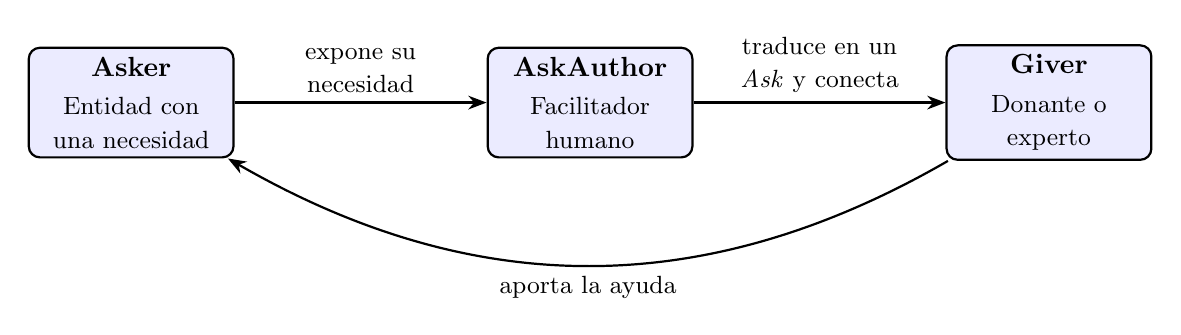
\begin{tikzpicture}[
  actor/.style={rectangle, rounded corners, draw=black, thick, fill=blue!8,
                 minimum width=2.6cm, minimum height=1.2cm, align=center}
]
  \node[actor] (asker) {\textbf{Asker}\\[2pt]\small Entidad con\\\small una necesidad};
  \node[actor, right=3.2cm of asker] (author) {\textbf{AskAuthor}\\[2pt]\small Facilitador\\\small humano};
  \node[actor, right=3.2cm of author] (giver) {\textbf{Giver}\\[2pt]\small Donante o\\\small experto};

  \draw[-{Stealth}, thick] (asker) -- node[above, align=center]{\small expone su\\\small necesidad} (author);
  \draw[-{Stealth}, thick] (author) -- node[above, align=center]{\small traduce en un\\\small \textit{Ask} y conecta} (giver);
  \draw[-{Stealth}, thick] (giver) to[out=-150, in=-30] node[below]{\small aporta la ayuda} (asker);
\end{tikzpicture}
\caption[Modelo relacional de AskingX]{Modelo relacional de AskingX.}
\label{fig:modelo-askingx}
\end{figure}

A medida que el éxito empírico de Bristol se consolidaba, surgió el reto de la escalabilidad territorial. Para evitar que el sistema dependiera exclusivamente de sus impulsores originales, el proceso se formalizó, dando lugar a \textit{AskingX} como un marco conceptual replicable. Este modelo se estructuró en tres niveles operativos: opciones (adaptaciones locales), estrategias (ejes de transformación) y acciones (prácticas observables). Asimismo, se estableció la división estricta de roles (\textit{Askers}, \textit{Givers} y \textit{AskAuthors}) para minimizar los obstáculos a la hora de replicar el sistema en nuevas ciudades \cite{canos_manley_2024}.

Es a partir de este modelo replicable cuando nace \textit{AskingValència}. Su aplicación local mantiene la esencia ágil y poco jerarquizada del proyecto original, aunque se enfrenta al reto de construir desde cero su propia red de usuarios. La puesta en marcha en Valencia ha servido para confirmar la teoría del modelo original: es imprescindible contar con facilitadores formados, es vital conseguir \textit{quick wins} (victorias tempranas) para que la gente confíe en el sistema y, fundamentalmente, se necesita una buena narrativa. Registrar y compartir las historias de éxito se ha convertido en la herramienta principal para atraer a nuevos participantes y hacer crecer el ecosistema de forma orgánica.
\section{Situación actual de la tecnología (Plataformas del Tercer Sector)}

La transformación digital ha impactado profundamente en la forma en que las organizaciones operan. Sin embargo, en el ámbito de la innovación social, la adopción tecnológica ha sido fragmentada y, a menudo, ha estado alejada de las dinámicas reales de los ecosistemas cívicos. Esta brecha no responde únicamente a un desinterés, sino a barreras estructurales bien documentadas: presupuestos ajustados y una capacidad digital interna limitada condicionan qué herramientas pueden permitirse realmente las entidades del tercer sector \cite{godefroid2024barriers}. Con esa salvedad presente, las soluciones de software orientadas a este ámbito pueden categorizarse en tres grandes grupos, todos ellos con limitaciones notables a la hora de implementar un modelo relacional como \textit{AskingX}:

\textbf{1. Plataformas de voluntariado y portales de conexión (\textit{matchmaking}):}
Este es el modelo predominante en Internet, funcionando esencialmente como un repositorio estático donde las ONG publican «ofertas» o necesidades y los ciudadanos se inscriben; son ejemplos representativos el portal español \textit{Hacesfalta.org}\footnote{\url{https://www.hacesfalta.org/}}, de la Fundación Hazloposible, que reúne a miles de entidades del tercer sector, y la plataforma internacional \textit{Idealist}\footnote{\url{https://www.idealist.org/}}, con presencia en numerosos países. Si bien son herramientas útiles para movilizaciones masivas, operan bajo una lógica puramente transaccional —muy similar a un portal de empleo corporativo—. Al delegar el emparejamiento a simples bases de datos, se debilita la labor de intermediación. Esta despersonalización dificulta la construcción del compromiso a largo plazo: un voluntario que no percibe apoyo organizativo ni una relación directa con el impacto de su contribución difícilmente desarrolla un vínculo duradero con la organización. En contextos de innovación cívica, este modelo transaccional resulta ineficaz.

\textbf{2. Sistemas de gestión institucional (ERPs y CRMs para ONG):}
Si bien los sistemas de gestión institucional actuales pueden considerarse técnicamente maduros, presentan barreras críticas de comunicación y carecen de una visión arquitectónica compartida, lo que deriva en escenarios de integración complejos que terminan aislando a las organizaciones entre sí. Entre las soluciones más extendidas en este ámbito figuran el CRM de código abierto \textit{CiviCRM}\footnote{\url{https://civicrm.org/}}, concebido específicamente para entidades sin ánimo de lucro, y \textit{Salesforce Nonprofit Cloud}\footnote{\url{https://www.salesforce.com/nonprofit/}}, ampliamente adoptado por grandes organizaciones del sector.

\textbf{3. Redes sociales genéricas y mensajería instantánea:}
Resulta habitual que las organizaciones acaben coordinando su actividad a través de aplicaciones de mensajería o redes sociales generalistas, por ser las herramientas que ya tienen a su alcance. Apoyar la coordinación cívica sobre infraestructuras comerciales conlleva, sin embargo, un coste poco visible: estas plataformas no se diseñaron para el bien común, sino para captar la atención del usuario, y dejan la actividad social sin trazabilidad ni control real sobre los datos \cite{civic_engagement_platforms}. En la práctica, esto expone a personas vulnerables a riesgos de vigilancia, demostrando que el marco del RGPD a menudo falla en protegerlas equitativamente en entornos digitales informales \cite{vanzoonen2022data}.

La Tabla~\ref{tab:comparativa-plataformas} sintetiza las diferencias entre estos tres enfoques y el modelo que se propone en este trabajo.

\begin{table}[ht]
\centering
\caption[Comparativa de soluciones del tercer sector]{Comparativa de soluciones del tercer sector.}
\label{tab:comparativa-plataformas}
\footnotesize
\renewcommand{\arraystretch}{1.4}
\begin{tabularx}{\textwidth}{%
  >{\raggedright\arraybackslash}p{3cm}%
  >{\raggedright\arraybackslash}X%
  >{\raggedright\arraybackslash}X%
  >{\raggedright\arraybackslash}X}
\toprule
\textbf{Enfoque} & \textbf{Emparejamiento} & \textbf{Mediación humana} & \textbf{Trazabilidad del impacto} \\
\midrule
Plataformas de \mbox{\textit{matchmaking}} & Automático, delegado a una base de datos & Mínima; el voluntario se autogestiona & Limitada, orientada a la inscripción \\
ERPs y CRMs para ONG & Manual e interno a cada organización & Burocrática, centrada en la gestión & Alta, pero aislada en silos \\
Redes sociales genéricas & Informal y viral, sin criterio & Inexistente & Nula, con riesgos para los datos \\
\textbf{AskingX (propuesta)} & Relacional, guiado por el \mbox{\textit{AskAuthor}} & Central; es el núcleo del modelo & Atómica, registrada en cada \mbox{\textit{Fulfillment}} \\
\bottomrule
\end{tabularx}
\end{table}

\section{Crítica al estado del arte}

La revisión del panorama tecnológico revela un patrón común a las tres categorías analizadas: la tendencia a que el \textit{software} ocupe el lugar de la mediación humana en vez de apoyarla. Las plataformas de \textit{matchmaking} delegan en un algoritmo una labor de intermediación que exige contexto y criterio; los ERPs resuelven la gestión interna pero no la conexión entre organizaciones; y las redes sociales aportan alcance a costa de la trazabilidad y la privacidad. Son herramientas válidas para los fines para los que se diseñaron, pero ninguna encaja con un modelo donde el valor reside precisamente en la relación de confianza que construye una persona.

Conviene matizar este diagnóstico para no caer en una simplificación. No se trata de que la tecnología sea ajena al tercer sector, ni de que estas plataformas carezcan de utilidad. El desajuste es más sutil: la mayoría de estas soluciones parten de una lógica transaccional —emparejar oferta y demanda— cuando lo que sostiene a un ecosistema como \textit{AskingX} es una lógica relacional. Esa diferencia de fondo es la que explica por qué una herramienta genérica, por buena que sea, rara vez se adapta bien a este contexto. La tecnología, en este ámbito, rinde mejor cuando actúa como una infraestructura discreta al servicio del facilitador, y no como el centro de la acción.

\section{Propuesta}

Ante este vacío, este trabajo plantea desarrollar una solución a medida en lugar de adaptar una herramienta existente. La idea rectora es sencilla: construir una plataforma que empodere al facilitador (\textit{AskAuthor}) en vez de reemplazarlo. En la práctica, esto se traduce en un sistema web ligero que asuma la parte mecánica del trabajo —el seguimiento del estado de cada petición, el control de quién puede hacer qué y el registro de las entregas— y reserve a la persona las tareas que requieren criterio humano: escuchar, interpretar y conectar.

De este planteamiento se derivan tres requisitos que guían el resto de la memoria. Primero, la herramienta debe reducir la carga administrativa en lugar de añadir más: una solución que acabe burocratizando el proceso resultaría contraproducente. Segundo, debe registrar el ciclo de vida de cada petición con la precisión suficiente para que el impacto sea auditable y, a partir de ahí, narrable. Y tercero, ha de ser segura y respetuosa con los datos de unos colectivos a menudo vulnerables. Los capítulos siguientes concretan cómo se aterrizan estas ideas en decisiones de análisis, diseño e implementación.
\chapter{Metodología de Desarrollo}
\section{Enfoque ágil e iterativo}

Para el desarrollo de este proyecto se ha optado por una metodología ágil e iterativa. Esta elección se justifica por la naturaleza del modelo AskingX, que requiere una adaptación constante a las necesidades de los actores sociales y permite obtener resultados funcionales desde las primeras etapas del proyecto.

Conviene una precisión honesta antes de continuar. Al tratarse de un proyecto individual, no se aplicaron las ceremonias formales de Scrum ni se empleó una herramienta específica de seguimiento de \textit{sprints}; el registro real de la evolución del trabajo lo constituye el historial de \textit{commits} del repositorio. Por ello, cuando en esta memoria se habla de \textit{Sprints} se hace referencia a iteraciones temáticas —de una duración aproximada de dos semanas cada una— organizadas en torno a un dominio concreto del sistema, más que a ciclos cronometrados con plazos rígidos. Las marcas de tiempo de los \textit{commits} ofrecen, de forma implícita, la traza de esa cadencia.

Cada iteración se centró en un área del sistema (gestión de usuarios, ciclo de vida de las peticiones, seguridad y control de acceso, entre otras) y recorrió las fases de análisis, modelado de datos, implementación y prueba antes de pasar a la siguiente. Este enfoque incremental permitió consolidar el núcleo arquitectónico del sistema antes de abordar las funcionalidades de mayor complejidad. El seguimiento se apoyó en reuniones periódicas con el tutor del trabajo, en las que se validaba lo construido y se reorientaban las prioridades de la siguiente iteración.

La naturaleza versátil de la metodología ha resultado fundamental para la evolución del sistema, permitiendo reajustar los requisitos a partir de la retroalimentación continua. Un ejemplo representativo de esta adaptación se produjo durante la definición del ciclo de vida de una petición (\textit{Ask}). Inicialmente, se planteó que la asignación de un voluntario (\textit{Match}) desencadenara de forma automatizada el cambio al estado de completado (\textit{Fulfilled}). Sin embargo, tras la validación con los \textit{stakeholders}, se concluyó que el hecho de que la conexión existiera no garantizaba el éxito de la donación. Por tanto, se redefinió este flujo iterativamente para introducir un patrón de \textit{Human-in-the-loop}, estableciendo que el trabajador social (\textit{AskAuthor}) debe monitorizar y confirmar manualmente la entrega efectiva de la ayuda. Este cambio arquitectónico pudo ser asimilado de forma natural gracias a la ausencia de rigidez de la metodología empleada.

A modo de mapa, la Tabla~\ref{tab:sprints} resume las cinco iteraciones en que se organizó el desarrollo; las secciones posteriores las detallan una a una.

\begin{table}[ht]
\centering
\caption[Resumen de las iteraciones de desarrollo]{Resumen de las iteraciones de desarrollo.}
\label{tab:sprints}
\footnotesize
\renewcommand{\arraystretch}{1.3}
\begin{tabularx}{\textwidth}{%
  c l%
  >{\raggedright\arraybackslash}X%
  >{\raggedright\arraybackslash}X}
\toprule
\textbf{Sprint} & \textbf{Fase} & \textbf{Foco principal} & \textbf{Resultado principal} \\
\midrule
1 & Backend & Modelado de datos y arquitectura base & Esquema \mbox{\textit{Prisma}} y base de datos relacional \\
2 & Backend & Seguridad, RBAC y autenticación & Autenticación JWT y \textit{middlewares} de rol \\
3 & Backend & Lógica relacional y \textit{endpoints} & Máquina de estados y validación con \mbox{\textit{Zod}} \\
4 & Frontend & Vistas y componentes base & Catálogo de componentes \mbox{\textit{React}} reutilizables \\
5 & Frontend & Integración con la API y estado & Tablero \textit{Kanban} y capa de servicios \\
\bottomrule
\end{tabularx}
\end{table}

\section{Herramientas de gestión y desarrollo}

Con el fin de dar soporte a la metodología ágil y garantizar la calidad del ciclo de desarrollo, se ha seleccionado un conjunto de herramientas acordes a los estándares actuales de la industria del \textit{software}. La Tabla~\ref{tab:herramientas} las recoge agrupadas según su función dentro del proyecto.

\begin{table}[ht]
\centering
\caption[Herramientas de gestión y desarrollo]{Herramientas de gestión y desarrollo.}
\label{tab:herramientas}
\footnotesize
\renewcommand{\arraystretch}{1.3}
\begin{tabularx}{\textwidth}{%
  >{\raggedright\arraybackslash}p{3.2cm}%
  >{\raggedright\arraybackslash}p{3.2cm}%
  >{\raggedright\arraybackslash}X}
\toprule
\textbf{Herramienta} & \textbf{Categoría} & \textbf{Uso en el proyecto} \\
\midrule
\textit{Git} y \textit{GitHub} & Control de versiones & Repositorio central; el historial de \textit{commits} sirve como registro de la evolución del proyecto \\
\textit{Visual Studio Code} & Entorno de desarrollo & Edición del código de \textit{backend} y \textit{frontend} \\
\textit{Postman} & Pruebas de API & Validación aislada de los \textit{endpoints} de la API REST \\
Herramientas de IA generativa & Prototipado & Generación de los \textit{mockups} iniciales de las vistas \\
\textit{Node.js} y \textit{Express} & \textit{Runtime} y \textit{framework} \textit{backend} & Lógica de servidor y exposición de la API REST \\
\textit{PostgreSQL} (\textit{Supabase}) & Base de datos & Persistencia relacional gestionada en la nube \\
\textit{Prisma ORM} & Acceso a datos & Mapeo objeto-relacional y diseño dirigido por modelos (\textit{Model-Driven Design}) \\
\textit{Zod} & Validación & Validación estricta de los esquemas de datos entrantes \\
\textit{React} y \textit{Vite} & \textit{Framework} y empaquetador \textit{frontend} & Interfaz SPA con recarga de módulos en caliente (HMR) \\
\textit{Tailwind CSS} & Estilos & Maquetación \textit{utility-first} basada en componentes \\
\bottomrule
\end{tabularx}
\end{table}



\section{Ejecución de Sprints: Fase Backend}

El desarrollo de la lógica del servidor (\textit{backend}) se estructuró en tres iteraciones principales. El objetivo de esta fase fue construir una Interfaz de Programación de Aplicaciones (API) RESTful robusta, capaz de gestionar las reglas de negocio propios del modelo AskingX antes de exponer cualquier funcionalidad a la interfaz de usuario.

\subsection{Sprint 1: Modelado de datos y arquitectura base}
La primera fase se dedicó íntegramente a la adaptación del diseño conceptual (diagramas UML) a un esquema de base de datos relacional físico. Para este propósito, se integró \textit{Prisma ORM}\footnote{\url{https://www.prisma.io/docs/}}, una herramienta de mapeo objeto-relacional. La adopción de esta tecnología supuso uno de los primeros retos técnicos del proyecto debido a la curva de aprendizaje inicial que requiere su lenguaje de definición de esquemas (\textit{schema.prisma}). 

Durante este ciclo, se implementaron decisiones arquitectónicas críticas para la escalabilidad del sistema. Por ejemplo, se estableció una relación de uno a muchos (1:N) entre las peticiones (\textit{Asks}) y los dominios de conocimiento (\textit{Domains}), garantizando una categorización estricta. Paralelamente, se modeló una relación de muchos a muchos (N:M) para gestionar las especialidades de los usuarios con rol de \textit{Connector} y \textit{Giver}, lo que permite al sistema reflejar la realidad multidisciplinar de los voluntarios. La sincronización de este esquema generó los artefactos necesarios para dotar al entorno de desarrollo de un tipado estricto.

\subsection{Sprint 2: Seguridad, RBAC y autenticación}
Una vez consolidada la capa de persistencia, el segundo \textit{Sprint} se centró en blindar el acceso a los recursos. Se diseñó un sistema de autenticación sin estado (\textit{stateless}) basado en el estándar JSON Web Tokens (JWT) \cite{jwt_rfc}, delegando el cifrado unidireccional de las contraseñas a la biblioteca \textit{Bcrypt}\footnote{\url{https://github.com/kelektiv/node.bcrypt.js}}.

El mayor esfuerzo de esta iteración recayó en la implementación de un Control de Acceso Basado en Roles (RBAC). Dado que el ecosistema AskingX interactúa con cuatro perfiles altamente diferenciados (\textit{Admin}, \textit{Author}, \textit{Connector} y \textit{Giver}), se desarrollaron \textit{middlewares} de interceptación al sistema de rutas de (\textit{Express}). Estos filtros no solo verifican la validez criptográfica del token, sino que evalúan los privilegios de la petición antes de ceder el control a la capa de servicios. De este modo, se garantizó estructuralmente que acciones críticas, como la creación de una petición de ayuda, quedaran restringidas exclusivamente al personal autorizado (\textit{AskAuthor}).

\subsection{Sprint 3: Lógica relacional y endpoints de negocio}
Este ciclo representó el núcleo de la complejidad del servidor. El reto principal fue doble: por un lado, asimilar y programar el intrincado flujo de estados de una petición (\textit{Ask}) entre los diferentes actores sociales; y por otro, dominar la librería \textit{Zod}\footnote{\url{https://zod.dev/}} para la validación estricta de esquemas de entrada. 

El uso conjunto de \textit{Zod} y \textit{Express} exigió la refactorización del manejo de errores globales del servidor, ya que inicialmente los fallos de validación en la estructura de los datos entrantes provocaban la caída del proceso de \textit{Node.js}. Se implementó una capa de control (\textit{Fail-Safe}) capaz de capturar estas excepciones y devolver códigos de estado HTTP 400 (\textit{Bad Request}) con descripciones semánticas.

En el ámbito del negocio, se programaron los controladores encargados de las transiciones de estado de las peticiones (desde \textit{CREATED} hasta \textit{FULFILLED}). Se implementaron medidas de seguridad avanzadas como el mecanismo \textit{Anti-Spoofing}, mediante el cual la API ignora cualquier identificador de autoría enviado en el cuerpo de la petición y lo sustituye por el identificador real extraído de la firma del token JWT. Finalmente, se consolidó el filtro de privacidad a nivel de consulta (\textit{Query-level filtering}), asegurando que, al solicitar el listado de peticiones, el motor de base de datos solo devuelva los registros que correspondan a la especialidad o propiedad de cada usuario.

\section{Planificación de Sprints: Fase Frontend}

Completado y documentado el \textit{backend}, el esfuerzo de desarrollo se trasladó a la construcción del cliente web (\textit{frontend}). Esta fase se planificó en dos ciclos de trabajo orientados a ofrecer una experiencia de usuario (UX) fluida, reactiva y tolerante a fallos.

\subsection{Sprint 4: Diseño de vistas (Mockups) y componentes base}
La cuarta iteración abordó la maquetación y estructura de la interfaz. Se seleccionó la librería \textit{React} (en su versión 19)\footnote{\url{https://react.dev/}} junto con el empaquetador \textit{Vite}\footnote{\url{https://vite.dev/}}, priorizando el rendimiento en el entorno de desarrollo mediante el reemplazo de módulos en caliente (HMR). El apartado visual se resolvió empleando \textit{Tailwind CSS}\footnote{\url{https://tailwindcss.com/}}, un marco de trabajo de utilidades que permitió evitar la saturación de archivos de estilos globales y aplicar principios de responsabilidad única a nivel de presentación.

Durante este \textit{Sprint}, se construyó un catálogo de componentes reutilizables (formularios dinámicos, modales, barras de navegación y tarjetas de estadística) respetando el principio DRY (\textit{Don't Repeat Yourself}). Uno de los desafíos técnicos destacables en la creación de los formularios fue la gestión algorítmica de zonas horarias (\textit{Timezones}). Para evitar la introducción de fechas inconsistentes en el campo de vencimiento (\textit{dueDate}), se programó una lógica de cálculo en tiempo real basada en la zona horaria local del navegador del cliente, bloqueando la selección de fechas pasadas nativamente en HTML5 y transformando posteriormente el dato al estándar ISO 8601 para su correcto almacenamiento.

\subsection{Sprint 5: Integración con la API y gestión del estado}
El último ciclo de desarrollo se dedicó a la interconexión asíncrona entre la interfaz construida y los \textit{endpoints} del servidor mediante la API \textit{Fetch}\footnote{\url{https://developer.mozilla.org/en-US/docs/Web/API/Fetch_API}}. Se extrajo toda la lógica de comunicación HTTP a una capa de servicios independiente (\textit{authService}, \textit{askService}, etc.), aislando a los componentes de la vista de la responsabilidad de gestionar peticiones de red.

La dificultad central de esta fase radicó en la programación defensiva de la aplicación. Se instruyó al código cliente para validar exhaustivamente las respuestas del servidor antes de renderizarlas en el Modelo de Objetos del Documento (DOM), evitando caídas críticas de la aplicación ante potenciales respuestas malformadas. Por último, se desarrolló la funcionalidad estrella para el rol del \textit{Connector}: un tablero interactivo basado en la metodología \textit{Kanban}. Haciendo uso de la API nativa de \textit{Drag and Drop} de HTML5\footnote{\url{https://developer.mozilla.org/en-US/docs/Web/API/HTML_Drag_and_Drop_API}}, se programó un sistema fluido y visual que permite a los coordinadores arrastrar tarjetas de peticiones entre distintas columnas, automatizando las llamadas al \textit{backend} para asignar voluntarios y gestionar las transiciones de estado en tiempo real.

\chapter{Análisis del Problema}

Antes de escribir una sola línea de código hubo que resolver un problema previo: traducir el modelo AskingX —que hasta ese momento vivía en la práctica diaria de los facilitadores— a un conjunto de requisitos concretos y verificables. Este capítulo recoge ese trabajo de análisis, desde la captura de requisitos hasta el estudio de riesgos, el marco legal y la viabilidad económica de la solución.

\section{Especificación de Requisitos}

La especificación parte de una particularidad del modelo que conviene fijar desde el principio, porque condiciona todo el diseño posterior: en AskingX no todos los actores implicados son usuarios del sistema. El \textit{Asker} —la entidad con una necesidad— es un sujeto pasivo, gestionado por el personal interno, que ni inicia sesión ni interactúa con la plataforma. Esta decisión, heredada del modelo relacional original, reduce de forma deliberada la superficie de exposición de datos de colectivos vulnerables.

\subsection{Actores del sistema}

Se distinguen cuatro perfiles con cuenta de usuario y un actor pasivo sin acceso:

\begin{itemize}
    \item \textbf{Administrador (\textit{Admin}).} Tiene control total. Aprueba o cancela las peticiones recién creadas, gestiona el personal interno y administra los dominios temáticos.
    \item \textbf{Autor de peticiones (\textit{AskAuthor}).} Trabaja con las entidades: registra \textit{Askers}, redacta sus peticiones y se encarga de las historias de impacto.
    \item \textbf{Conector (\textit{Connector}).} Es el «solucionador»: empareja donantes con peticiones abiertas y registra las entregas de ayuda.
    \item \textbf{Donante (\textit{Giver}).} Aporta los recursos. Sus datos y disponibilidad se almacenan en el sistema, pero su interacción directa es mínima.
    \item \textbf{Solicitante (\textit{Asker}).} Actor pasivo, sin cuenta. Representa a la ONG, colegio o persona vulnerable cuya necesidad se digitaliza.
\end{itemize}

\subsection{Requisitos funcionales}

La Tabla~\ref{tab:requisitos-funcionales} recoge los requisitos funcionales (RF) que el sistema debe satisfacer. Se han extraído directamente del flujo de trabajo real de la iniciativa.

\begin{table}[ht]
\centering
\caption[Requisitos funcionales del sistema]{Requisitos funcionales del sistema.}
\label{tab:requisitos-funcionales}
\footnotesize
\renewcommand{\arraystretch}{1.3}
\begin{tabularx}{\textwidth}{%
  >{\raggedright\arraybackslash}p{1.4cm}%
  >{\raggedright\arraybackslash}X}
\toprule
\textbf{Código} & \textbf{Descripción} \\
\midrule
RF-01 & El \textit{AskAuthor} puede crear, consultar y actualizar los perfiles de las entidades solicitantes (\textit{Askers}). \\
RF-02 & El \textit{AskAuthor} crea peticiones (\textit{Asks}) en nombre de un \textit{Asker}; toda petición nace en estado \textit{CREATED}. \\
RF-03 & El sistema admite cuatro tipos de petición (\textit{THINGS}, \textit{TIME}, \textit{EXPERTISE} y \textit{SERVICES}), cada uno con sus campos propios. \\
RF-04 & El \textit{Admin} aprueba una petición —que pasa a \textit{OPEN}— o la cancela antes de hacerla pública. \\
RF-05 & El \textit{Connector} vincula uno o varios \textit{Givers} a una petición abierta, que pasa a \textit{MATCHED}. \\
RF-06 & El \textit{Connector} registra entregas parciales (\textit{Fulfillments}) que asocian un \textit{Giver} con la ayuda aportada. \\
RF-07 & El sistema acumula lo entregado y, al alcanzar o superar lo solicitado, marca la petición como \textit{FULFILLED}; además, impide registrar entregas que excedan lo pedido. \\
RF-08 & Un proceso programado marca como \textit{EXPIRED} las peticiones \textit{OPEN} o \textit{MATCHED} cuya fecha límite ha vencido. \\
RF-09 & El \textit{AskAuthor} puede descartar o republicar una petición caducada. \\
RF-10 & El \textit{AskAuthor} y el \textit{Admin} generan, revisan y publican Historias de Impacto a partir de peticiones completadas, con apoyo de un modelo de lenguaje. \\
RF-11 & El \textit{Admin} gestiona el personal interno (alta, edición y baja lógica) y los dominios temáticos. \\
RF-12 & El sistema autentica a los usuarios y restringe cada acción según su rol (RBAC). \\
RF-13 & Cada usuario puede operar en español, valenciano o inglés. \\
\bottomrule
\end{tabularx}
\end{table}

\subsection{Requisitos no funcionales}

Más allá de lo que el sistema hace, importa cómo lo hace. La Tabla~\ref{tab:requisitos-no-funcionales} resume los requisitos no funcionales (RNF), que en un proyecto que maneja datos de personas vulnerables tienen un peso especial.

\begin{table}[ht]
\centering
\caption[Requisitos no funcionales del sistema]{Requisitos no funcionales del sistema.}
\label{tab:requisitos-no-funcionales}
\footnotesize
\renewcommand{\arraystretch}{1.3}
\begin{tabularx}{\textwidth}{%
  >{\raggedright\arraybackslash}p{1.4cm}%
  >{\raggedright\arraybackslash}p{3cm}%
  >{\raggedright\arraybackslash}X}
\toprule
\textbf{Código} & \textbf{Categoría} & \textbf{Descripción} \\
\midrule
RNF-01 & Seguridad & Autenticación sin estado mediante JWT y contraseñas cifradas con \textit{bcrypt}. \\
RNF-02 & Privacidad & Baja lógica de usuarios (sin borrado físico) y un modelo en el que el \textit{Asker} no dispone de cuenta, lo que reduce la exposición de datos. \\
RNF-03 & Integridad & Acceso a datos mediante un ORM fuertemente tipado que previene la inyección SQL. \\
RNF-04 & Usabilidad & Interfaz \textit{mobile-first} y de página única (SPA), sin recargas entre vistas. \\
RNF-05 & Mantenibilidad & Arquitectura por capas (Rutas, Controladores y Servicios) con responsabilidades separadas. \\
RNF-06 & Portabilidad & \textit{Backend} autónomo (\textit{standalone}), desplegable en plataformas \textit{cloud} (PaaS). \\
RNF-07 & Internacionalización & Soporte de tres idiomas en la interfaz de usuario. \\
\bottomrule
\end{tabularx}
\end{table}

\section{Modelado Conceptual}

Con los requisitos sobre la mesa, el siguiente paso fue modelar la información que el sistema debía manejar. El dominio gira en torno a una entidad central, la petición (\textit{Ask}), a la que se conectan el resto de conceptos. La Figura~\ref{fig:modelo-conceptual} muestra las entidades principales y las relaciones que las unen.

\begin{figure}[htbp]
\centering
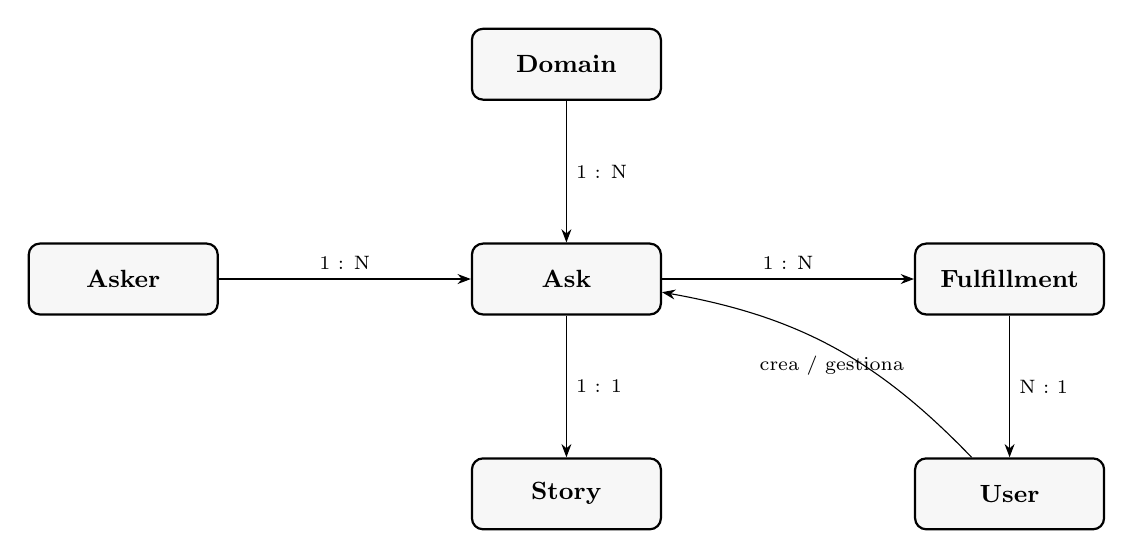
\begin{tikzpicture}[
  ent/.style={rectangle, draw=black, thick, fill=gray!6, rounded corners,
              minimum width=2.4cm, minimum height=0.9cm, align=center, font=\small},
  rel/.style={font=\scriptsize}
]
  \node[ent] (ask) {\textbf{Ask}};
  \node[ent, left=3.2cm of ask] (asker) {\textbf{Asker}};
  \node[ent, above=1.8cm of ask] (domain) {\textbf{Domain}};
  \node[ent, right=3.2cm of ask] (fulfillment) {\textbf{Fulfillment}};
  \node[ent, below=1.8cm of ask] (story) {\textbf{Story}};
  \node[ent, below=1.8cm of fulfillment] (user) {\textbf{User}};

  \draw[-{Stealth}] (asker) -- node[rel, above]{1 : N} (ask);
  \draw[-{Stealth}] (domain) -- node[rel, right]{1 : N} (ask);
  \draw[-{Stealth}] (ask) -- node[rel, above]{1 : N} (fulfillment);
  \draw[-{Stealth}] (fulfillment) -- node[rel, right]{N : 1} (user);
  \draw[-{Stealth}] (ask) -- node[rel, right]{1 : 1} (story);
  \draw[-{Stealth}] (user) to[bend right=18] node[rel, below]{crea / gestiona} (ask);
\end{tikzpicture}
\caption[Modelo conceptual del dominio]{Modelo conceptual del dominio.}
\label{fig:modelo-conceptual}
\end{figure}

Las relaciones reflejan la lógica del modelo. Un \textit{Asker} puede acumular varias peticiones a lo largo del tiempo, pero cada petición pertenece a un único solicitante y se clasifica en un solo dominio temático (\textit{Domain}). La relación más característica es la que une la petición con sus entregas: un \textit{Ask} se asocia a cero o varios \textit{Fulfillments}, lo que permite registrar la ayuda de forma progresiva en lugar de exigir que se complete de una sola vez. Cada entrega, a su vez, queda vinculada de manera atómica a un \textit{Giver} concreto, garantizando la trazabilidad. Por último, una petición completada puede dar lugar a una única Historia de Impacto (\textit{Story}).

La entidad \textit{User} merece una observación. En lugar de crear una tabla por rol, se ha optado por una única entidad de usuario cualificada por un atributo de rol (\textit{Admin}, \textit{AskAuthor}, \textit{Connector} o \textit{Giver}). Esta decisión simplifica el modelo y se justifica en detalle en el capítulo de diseño; aquí basta señalar que un mismo \textit{User} participa en el dominio de formas distintas según su rol: creando peticiones, gestionándolas o aportando entregas.

\section{Análisis del marco legal y ético (RGPD y uso de IA)}

Trabajar con datos de organizaciones, voluntarios y, sobre todo, de personas en situación de vulnerabilidad obliga a tomarse en serio la protección de datos. En este proyecto no se ha tratado como un trámite final, sino como una restricción de diseño presente desde el modelado.

\subsection{Cumplimiento del RGPD}

El sistema trata datos de carácter personal en tres puntos: los datos de contacto de las entidades solicitantes (persona de contacto, teléfono y correo), los del personal interno con cuenta y las notas de disponibilidad de los donantes. Para ajustarse al Reglamento General de Protección de Datos se han aplicado varios principios de forma concreta.

El primero es la \textbf{minimización}. Solo se almacenan los campos estrictamente necesarios para operar, y aquí el modelo ayuda por sí mismo: como el \textit{Asker} no tiene cuenta ni inicia sesión, su huella de datos en el sistema es mínima. El segundo es la \textbf{limitación del acceso}: la política RBAC, reforzada con un filtrado a nivel de consulta, garantiza que cada perfil solo vea la información que le compete, evitando que un dato circule más allá de quien lo necesita. La seguridad de las credenciales se aborda con el cifrado de contraseñas y la autenticación por token, descritos en el capítulo de diseño.

Hay un punto que conviene reconocer abiertamente, porque tiene matices. La baja de usuarios se realiza de forma lógica (\textit{isActive: false}) y no física, una decisión tomada para preservar la trazabilidad histórica de las intervenciones. Esto convive con el derecho de supresión que reconoce el RGPD: para un borrado completo a petición del interesado sería necesario un procedimiento adicional de eliminación física, que queda señalado como mejora. El énfasis en estas cautelas no es casual; la literatura advierte de que el marco regulatorio a menudo protege de forma desigual a los colectivos más vulnerables en entornos digitales \cite{vanzoonen2022data}, precisamente los que atiende esta plataforma.

\subsection{Uso ético de la Inteligencia Artificial}

El único componente de IA del sistema es el módulo que redacta Historias de Impacto a partir de peticiones ya completadas. Su alcance es deliberadamente limitado, y eso es importante para las implicaciones éticas.

La IA \textbf{no toma decisiones que afecten a las personas}: no decide emparejamientos, no perfila usuarios ni prioriza necesidades. Se limita a generar un texto narrativo. Además, opera bajo un esquema de \textit{Human-in-the-loop}: ninguna historia se publica de forma automática, sino que un \textit{AskAuthor} o el \textit{Admin} la revisan y aprueban antes de hacerla visible. Bajo la clasificación del Reglamento Europeo de Inteligencia Artificial, un uso de este tipo —generación de texto con supervisión humana— se sitúa en la categoría de riesgo mínimo.

Queda, no obstante, una consideración honesta: la generación delega en un modelo de lenguaje externo, lo que implica enviar cierta información a un tercero. La mitigación adoptada es doble: enviar al modelo solo los datos imprescindibles para construir la narrativa y mantener la revisión humana como filtro final. La anonimización sistemática de los datos enviados al modelo se contempla como línea de mejora.

\section{Análisis de Riesgos}

Todo proyecto de software, y más uno desarrollado por una sola persona en un plazo acotado, convive con riesgos. Identificarlos pronto permitió tomar decisiones de diseño que los redujeran en lugar de descubrirlos tarde. La Tabla~\ref{tab:riesgos} recoge los principales, valorados según su probabilidad e impacto, junto con la medida de mitigación adoptada.

\begin{table}[ht]
\centering
\caption[Análisis de riesgos del proyecto]{Análisis de riesgos del proyecto.}
\label{tab:riesgos}
\footnotesize
\renewcommand{\arraystretch}{1.3}
\begin{tabularx}{\textwidth}{%
  >{\raggedright\arraybackslash}p{0.9cm}%
  >{\raggedright\arraybackslash}X%
  >{\raggedright\arraybackslash}p{1.5cm}%
  >{\raggedright\arraybackslash}p{1.3cm}%
  >{\raggedright\arraybackslash}X}
\toprule
\textbf{ID} & \textbf{Riesgo} & \textbf{Prob.} & \textbf{Impacto} & \textbf{Mitigación} \\
\midrule
R1 & Caída o cambio del servicio externo de IA & Media & Medio & Mecanismo de reserva: si el modelo falla, se genera la historia con una plantilla local \\
R2 & Fuga o exposición de datos personales & Baja & Alto & RBAC, autenticación por token, minimización y filtrado por consulta \\
R3 & Pérdida de datos & Baja & Alto & Base de datos gestionada en la nube, que delega en el proveedor la gestión de la infraestructura \\
R4 & Baja adopción por parte de los facilitadores & Media & Alto & Diseño centrado en reducir carga y una interfaz sencilla \\
R5 & Alcance excesivo (\textit{scope creep}) en un proyecto individual & Alta & Medio & Priorización por iteraciones y construcción de un núcleo funcional primero \\
R6 & Transferencia de datos a un tercero (modelo de lenguaje) & Media & Medio & Envío del mínimo de datos imprescindibles y revisión humana previa \\
R7 & Curva de aprendizaje de tecnologías nuevas & Media & Bajo & Estudio previo de la documentación y prototipos rápidos \\
\bottomrule
\end{tabularx}
\end{table}

\section{Identificación y análisis de soluciones posibles}

Definido el problema, quedaba decidir el «cómo» antes de empezar a programar. Se valoraron dos caminos de fondo y un par de decisiones técnicas asociadas.

\subsection{Alternativa A: adaptar una solución existente}

La vía rápida habría sido apoyarse en un CRM para ONG o en una herramienta \textit{no-code} de propósito general. La ventaja es evidente: puesta en marcha casi inmediata. Pero, como ya se argumentó en el Capítulo 2, estas herramientas parten de una lógica transaccional o de gestión interna que no encaja con el flujo relacional de AskingX. Modelar sobre ellas la máquina de estados de las peticiones o el control de sobredonación habría resultado forzado, y además habría introducido dependencia de un proveedor y posibles costes de licencia.

\subsection{Alternativa B: desarrollo a medida}

La segunda opción —la finalmente elegida— era construir una aplicación full-stack propia. Tiene un coste claro: más tiempo de desarrollo. A cambio, ofrece justo lo que el proyecto necesitaba: un ajuste total al modelo, control directo sobre los datos (algo nada menor dado el peso del RGPD en este contexto), ausencia de licencias y libertad para desplegar en cualquier proveedor \textit{cloud}.

\subsection{Decisiones técnicas asociadas}

La elección del desarrollo a medida arrastró dos decisiones de calado. La primera, el tipo de base de datos: frente a un almacén documental (NoSQL), se optó por un modelo relacional (PostgreSQL). El dominio es intensamente relacional —peticiones ligadas a solicitantes, dominios, entregas y donantes—, y la integridad referencial de una base relacional encaja mucho mejor con esa realidad que la flexibilidad de un documento. La segunda, la arquitectura: en lugar de microservicios, se eligió un monolito modular organizado por capas. Para un producto mínimo viable desarrollado por una sola persona, esta opción aporta la mantenibilidad buscada sin la complejidad operativa que implicaría distribuir el sistema.

\section{Solución propuesta}

A la luz de este análisis, la solución que se desarrolla es una aplicación web full-stack a medida. El servidor se construye con Node.js y Express siguiendo una arquitectura en capas; la persistencia recae en PostgreSQL a través de Prisma; y el cliente es una aplicación de página única en React. Sobre esta base se asientan los elementos diferenciales del proyecto: la autenticación con JWT y el control de acceso por roles, la máquina de estados que gobierna el ciclo de vida de las peticiones y el módulo de generación de historias asistido por IA y supervisado. El detalle de cómo se materializa cada una de estas piezas es el objeto del Capítulo 5.

\section{Plan de Trabajo}

El trabajo se organizó en las iteraciones descritas en el Capítulo 3, repartidas a lo largo de algo más de siete semanas de desarrollo efectivo, entre finales de abril y principios de junio de 2026. La Figura~\ref{fig:gantt} representa esa planificación en un diagrama de Gantt, con la particularidad de que la redacción de la memoria avanzó en paralelo al desarrollo, apoyándose en notas técnicas que se iban registrando al cerrar cada iteración.

\begin{figure}[htbp]
\centering
\begin{ganttchart}[
  vgrid, hgrid,
  bar label font=\footnotesize,
  title label font=\footnotesize,
  bar/.style={fill=blue!30, draw=blue!50!black},
  y unit chart=0.55cm,
  y unit title=0.6cm
]{1}{8}
\gantttitle{Abril}{2}\gantttitle{Mayo}{4}\gantttitle{Junio}{2} \\
\gantttitle{S1}{1}\gantttitle{S2}{1}\gantttitle{S3}{1}\gantttitle{S4}{1}\gantttitle{S5}{1}\gantttitle{S6}{1}\gantttitle{S7}{1}\gantttitle{S8}{1} \\
\ganttbar{Análisis y diseño}{1}{1} \\
\ganttbar{Sprint 1: Modelado y BD}{1}{2} \\
\ganttbar{Sprint 2: Seguridad y RBAC}{3}{3} \\
\ganttbar{Sprint 3: Lógica y endpoints}{3}{4} \\
\ganttbar{Sprint 4: Frontend base}{4}{5} \\
\ganttbar{Sprint 5: Integración y Kanban}{5}{6} \\
\ganttbar{Ajustes y pruebas}{6}{7} \\
\ganttbar{Redacción de la memoria}{2}{8}
\end{ganttchart}
\caption[Diagrama de Gantt del proyecto]{Diagrama de Gantt del proyecto.}
\label{fig:gantt}
\end{figure}

\section{Presupuesto}

Aunque se trata de un proyecto académico, resulta ilustrativo estimar cuánto costaría su desarrollo en un contexto profesional. El cálculo se apoya en las horas de trabajo dedicadas, valoradas a la tarifa de un desarrollador junior, y parte de una premisa que abarata notablemente el resultado: todo el software empleado es de código abierto o se ha usado dentro de capas gratuitas, por lo que el coste en licencias es nulo.

El primer paso fue estimar la dedicación real, repartida entre las mismas fases que estructuran el plan de trabajo. La Tabla~\ref{tab:horas} recoge ese desglose, que suma 415 horas. La cifra se sitúa por encima de la carga nominal mínima de un Trabajo de Fin de Grado y refleja el esfuerzo que supuso aprender las tecnologías sobre la marcha, depurar la lógica de negocio y redactar la memoria en paralelo al desarrollo.

\begin{table}[ht]
\centering
\caption[Dedicación estimada por fases]{Dedicación estimada por fases.}
\label{tab:horas}
\footnotesize
\renewcommand{\arraystretch}{1.3}
\begin{tabularx}{\textwidth}{%
  >{\raggedright\arraybackslash}X%
  >{\raggedleft\arraybackslash}p{3cm}}
\toprule
\textbf{Fase} & \textbf{Dedicación (h)} \\
\midrule
Análisis y diseño & 30 \\
Sprint 1: Modelado de datos y base de datos & 40 \\
Sprint 2: Seguridad, RBAC y autenticación & 35 \\
Sprint 3: Lógica de negocio y \textit{endpoints} & 50 \\
Sprint 4: \textit{Frontend} y componentes base & 45 \\
Sprint 5: Integración y tablero \textit{Kanban} & 50 \\
Ajustes y pruebas & 35 \\
Redacción de la memoria & 130 \\
\midrule
\textbf{Total} & \textbf{415} \\
\bottomrule
\end{tabularx}
\end{table}

A partir de esa dedicación, la Tabla~\ref{tab:presupuesto} traslada las horas a coste y añade el resto de partidas.

\begin{table}[ht]
\centering
\caption[Presupuesto estimado del proyecto]{Presupuesto estimado del proyecto.}
\label{tab:presupuesto}
\footnotesize
\renewcommand{\arraystretch}{1.3}
\begin{tabularx}{\textwidth}{%
  >{\raggedright\arraybackslash}X%
  >{\raggedright\arraybackslash}p{6cm}%
  >{\raggedleft\arraybackslash}p{2cm}}
\toprule
\textbf{Concepto} & \textbf{Detalle} & \textbf{Coste} \\
\midrule
Recursos humanos & 415 h de desarrollo a 15 €/h (desarrollador junior) & 6\,225 € \\
Amortización de equipo & Portátil (\textasciitilde 900 €, 4 años de vida útil, \textasciitilde 3,5 meses de uso) & 65 € \\
Software y servicios & Herramientas de código abierto y capas gratuitas (Supabase, Gemini, GitHub) & 0 € \\
\midrule
\textbf{Total} & & \textbf{6\,290 €} \\
\bottomrule
\end{tabularx}
\end{table}

El desglose deja claro que el grueso del coste es la mano de obra. La práctica ausencia de gastos en infraestructura y licencias no es casual, sino consecuencia directa de las decisiones tecnológicas tomadas: apostar por un ecosistema de código abierto mantiene el coste de entrada muy bajo, un factor especialmente relevante para una iniciativa del tercer sector con recursos limitados.

\chapter{Diseño de la solución}

Una vez analizado el problema y justificada la opción de un desarrollo a medida, este capítulo aterriza esas decisiones en el diseño concreto de la solución. Se parte de la pila tecnológica elegida y su justificación, se describe a continuación la arquitectura que organiza el sistema y, por último, se detallan los elementos de diseño más característicos: el modelo de datos, el ciclo de vida de las peticiones y las reglas de negocio que lo gobiernan.

\section{Tecnología Utilizada}

La elección de las tecnologías no respondió a una preferencia arbitraria, sino a los requisitos fijados en el capítulo anterior: una solución mantenible, segura, portable y de coste de licencias nulo. Todas las piezas seleccionadas son de código abierto o cuentan con una capa de uso gratuita, lo que resulta coherente con el contexto de una iniciativa del tercer sector. La Figura~\ref{fig:stack} resume la pila tecnológica organizada por capas, desde el cliente hasta la persistencia.

\begin{figure}[htbp]
\centering
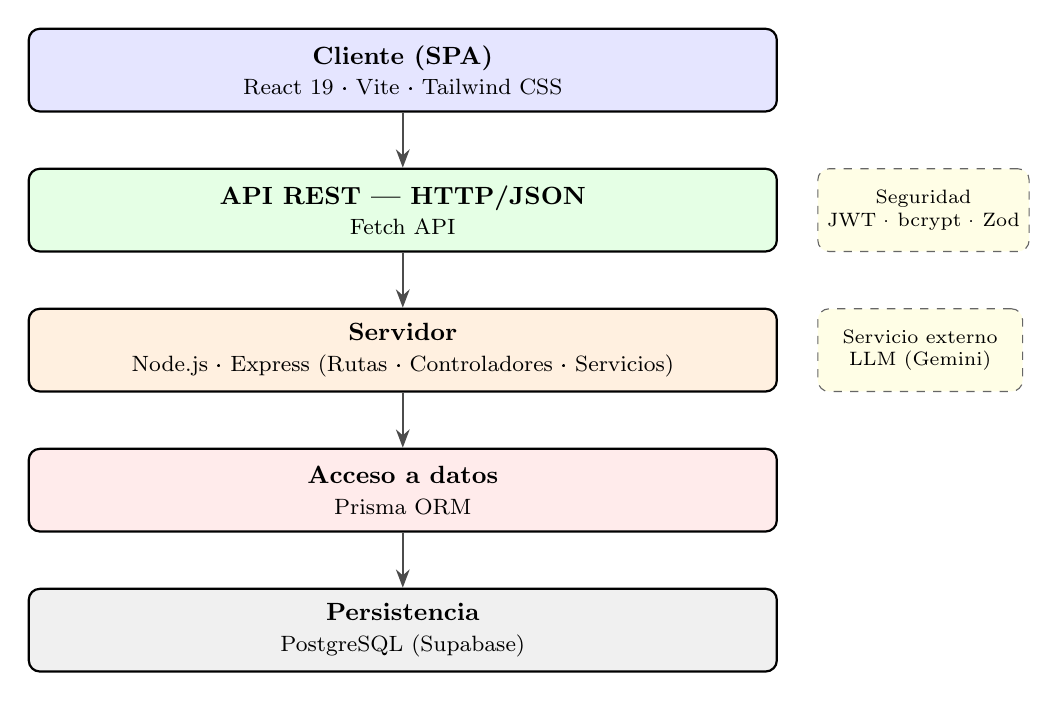
\begin{tikzpicture}[
  layer/.style={rectangle, rounded corners, draw=black, thick,
                minimum width=9.5cm, minimum height=1.05cm, align=center, font=\small},
  side/.style={rectangle, rounded corners, draw=black!60, dashed, fill=yellow!10,
               minimum width=2.6cm, minimum height=1.05cm, align=center, font=\scriptsize},
  flow/.style={-{Stealth}, thick, gray!60!black}
]
  \node[layer, fill=blue!10] (cli) {\textbf{Cliente (SPA)}\\\footnotesize React 19 · Vite · Tailwind CSS};
  \node[layer, fill=green!10, below=0.7cm of cli] (api) {\textbf{API REST --- HTTP/JSON}\\\footnotesize Fetch API};
  \node[layer, fill=orange!12, below=0.7cm of api] (srv) {\textbf{Servidor}\\\footnotesize Node.js · Express (Rutas · Controladores · Servicios)};
  \node[layer, fill=red!8, below=0.7cm of srv] (orm) {\textbf{Acceso a datos}\\\footnotesize Prisma ORM};
  \node[layer, fill=gray!12, below=0.7cm of orm] (db) {\textbf{Persistencia}\\\footnotesize PostgreSQL (Supabase)};

  \draw[flow] (cli) -- (api);
  \draw[flow] (api) -- (srv);
  \draw[flow] (srv) -- (orm);
  \draw[flow] (orm) -- (db);

  \node[side, right=0.5cm of api.east, anchor=west] (sec) {Seguridad\\JWT · bcrypt · Zod};
  \node[side, right=0.5cm of srv.east, anchor=west] (ia) {Servicio externo\\LLM (Gemini)};
\end{tikzpicture}
\caption[Pila tecnológica de la solución]{Pila tecnológica de la solución.}
\label{fig:stack}
\end{figure}

\subsection{Cliente}

La interfaz se ha construido como una aplicación de página única (SPA) con la biblioteca \textit{React} en su versión 19, empaquetada con \textit{Vite}. React aporta un modelo declarativo basado en componentes que encaja con la necesidad de reutilizar elementos de interfaz (formularios, modales, tarjetas) y de renderizar la vista de forma condicional según el rol del usuario. \textit{Vite}, por su parte, se eligió frente a empaquetadores más tradicionales por su servidor de desarrollo con recarga de módulos en caliente (HMR), que reduce de forma notable el tiempo del ciclo editar-comprobar. El apartado visual se resuelve con \textit{Tailwind CSS}, un marco de utilidades que mantiene los estilos junto al \textit{markup} de cada componente y evita el crecimiento descontrolado de hojas de estilo globales.

\subsection{Comunicación: API REST}

Cliente y servidor se comunican a través de una API que sigue el estilo arquitectónico REST \cite{fielding_rest}, intercambiando exclusivamente datos en formato JSON sobre HTTP. Este estilo, sin estado y orientado a recursos, encaja de forma natural con el dominio del problema —las entidades del modelo (peticiones, entregas, usuarios) se exponen como recursos identificables— y permite desacoplar por completo la evolución del cliente y la del servidor. Del lado del cliente, las llamadas se realizan con la API nativa \textit{Fetch}, evitando dependencias adicionales.

\subsection{Servidor}

El servidor se ha desarrollado sobre el entorno de ejecución \textit{Node.js} con el marco de trabajo \textit{Express}\footnote{\url{https://expressjs.com/}}. La combinación es un estándar de facto para construir APIs REST en JavaScript y permite mantener un único lenguaje en todo el proyecto, lo que reduce la fricción de contexto entre cliente y servidor. \textit{Express} aporta, además, un modelo de \textit{middlewares} que resulta idóneo para implementar de forma transversal la autenticación y el control de acceso por roles, tal como se describe en la sección de arquitectura.

\subsection{Persistencia y acceso a datos}

La persistencia recae en una base de datos relacional \textit{PostgreSQL}, alojada en el servicio gestionado \textit{Supabase} dentro de su capa gratuita. Como ya se justificó en el análisis, la naturaleza intensamente relacional del dominio hace preferible un modelo relacional, con integridad referencial garantizada, frente a un almacén documental. El acceso a los datos no se realiza con SQL directo, sino a través de \textit{Prisma ORM} (versión 5), un mapeador objeto-relacional fuertemente tipado. Prisma aporta dos ventajas decisivas: genera un cliente tipado a partir del esquema, lo que traslada numerosos errores a tiempo de compilación, y parametriza automáticamente las consultas, neutralizando los ataques de inyección SQL.

\subsection{Seguridad}

La seguridad se apoya en tres bibliotecas. La autenticación se resuelve con \textit{JSON Web Tokens} (JWT) \cite{jwt_rfc}, que permiten un esquema de sesión sin estado adecuado para una API REST. Las contraseñas nunca se almacenan en claro: se cifran de forma unidireccional con \textit{bcrypt}, cuyo factor de coste configurable lo hace resistente a ataques de fuerza bruta. Por último, toda entrada que llega al servidor se valida con \textit{Zod}, que define esquemas estrictos y rechaza las peticiones malformadas antes de que alcancen la lógica de negocio.

\subsection{Servicio de Inteligencia Artificial}

La generación de las Historias de Impacto delega en un modelo de lenguaje (LLM) accesible mediante API. Se ha integrado a través de la capa de servicios, de modo que el resto del sistema permanece ajeno a los detalles del proveedor concreto y este podría sustituirse sin afectar a la lógica de negocio. Como se detalló en el análisis del marco ético, esta integración opera siempre bajo supervisión humana y enviando al modelo únicamente la información imprescindible.

\section{Arquitectura del Sistema}

El diseño arquitectónico de la plataforma AskingX se fundamenta en el patrón Cliente-Servidor, estableciendo un claro desacoplamiento entre la interfaz de usuario (\textit{Frontend}) y la lógica de negocio y persistencia de datos (\textit{Backend}). 

Se ha optado por desarrollar el sistema de tal manera que opere de forma independiente (\textit{standalone}), garantizando su viabilidad como producto autónomo y facilitando su despliegue en infraestructuras \textit{cloud} estandarizadas (PaaS), dejando así una potencial integración con los sistemas heredados de las ONG como una línea de trabajo futuro.

\subsection{Capa de presentación (\textit{Frontend})}

La interfaz es una aplicación de página única (SPA) construida con React y Vite: el navegador descarga los recursos una sola vez y, a partir de ahí, actualiza la vista intercambiando datos en JSON con el servidor sin recargar el documento. El componente de gestión más característico es el tablero \textit{Kanban}, que organiza las peticiones por estado y permite arrastrarlas entre columnas para avanzar el flujo.

La vista es consciente del rol del usuario autenticado. Cada uno de los cuatro perfiles —\textit{Admin}, \textit{AskAuthor}, \textit{Connector} y \textit{Giver}— recibe un conjunto diferente de vistas y controles, de modo que el principio RBAC del servidor se refleja también en lo que cada usuario puede ver y hacer en la interfaz.

\subsection{Capa de Lógica de Negocio y Enrutamiento (\textit{Backend})}
El servidor se desarrolla sobre Node.js con Express y se organiza en tres capas con responsabilidades estrictamente separadas:

\begin{itemize}
    \item \textbf{Rutas (\textit{Routes}):} Declaran los \textit{endpoints} de la API y encadenan los \textit{middlewares} de autenticación y rol antes de ceder el paso al controlador.
    \item \textbf{Controladores (\textit{Controllers}):} Validan la entrada con \textit{Zod} y traducen entre HTTP y el dominio. Si la validación falla, devuelven un error 400 sin que la petición alcance la lógica de negocio.
    \item \textbf{Servicios (\textit{Services}):} Concentran la lógica de negocio: la máquina de estados, el control de sobredonación y la generación de historias de impacto.
\end{itemize}

\subsection{Gestión de Identidad y Seguridad}
La autenticación se basa en JSON Web Tokens (JWT): tras el inicio de sesión, el servidor emite un \textit{token} firmado que el cliente adjunta en la cabecera \texttt{Authorization: Bearer} de cada petición. Dos \textit{middlewares} en cadena verifican la firma del \textit{token} y comprueban que el rol del usuario esté autorizado para la ruta; el administrador dispone de paso franco en todos los casos.

Cabe destacar que solo los roles gestores —\textit{Connector} y \textit{AskAuthor}— pueden registrar entregas (\textit{Fulfillments}). El \textit{Giver}, aunque es el sujeto de la acción, no tiene permisos de escritura sobre ellas. Esta restricción deliberada garantiza que ninguna entrega quede confirmada en el sistema sin que un gestor la haya verificado previamente.

\subsection{Capa de Persistencia y Acceso a Datos}
La persistencia recae en PostgreSQL, accedida a través de Prisma ORM (versión 5). El cliente tipado que genera Prisma a partir del esquema desplaza muchos errores a tiempo de compilación y parametriza las consultas de forma automática, neutralizando la inyección SQL.

Para gestionar los cuatro tipos de petición en una sola tabla, el modelo aplica herencia de tabla única (\textit{Single-Table Inheritance}): la entidad \textit{Ask} dispone de cuatro campos especializados opcionales, de los cuales solo se rellena el que corresponde al tipo. Esto evita \textit{JOINs} al listar peticiones de tipos distintos y mantiene el esquema compacto.

\section{Diseño Detallado}

Establecida la pila tecnológica y la arquitectura por capas, esta sección desciende al detalle de diseño que da forma al sistema. Se abordan, en este orden, el modelo de datos que materializa el dominio, el ciclo de vida de la petición como máquina de estados, las reglas de negocio que el diseño debe garantizar, un conjunto de decisiones transversales que condicionan la experiencia de uso y, por último, las pautas que guían el diseño de la interfaz. Conviene una aclaración de alcance: este capítulo describe \textit{qué} se diseñó y por qué; el detalle de \textit{cómo} se programó cada pieza —el código, las consultas y los \textit{middlewares}— se reserva para el Capítulo 6.

\subsection{Modelo de datos}

El modelo conceptual presentado en el Capítulo 4 fijaba las entidades del dominio y sus relaciones de forma abstracta. El diseño detallado lo concreta en un modelo de clases que incorpora los atributos, los tipos de dato y las claves que finalmente se trasladan al esquema de \textit{Prisma}. La Figura~\ref{fig:diagrama-clases} recoge ese modelo estructural completo; los campos opcionales se marcan con \texttt{?} y la entidad \textit{AppConfig} se omite por no mantener asociaciones con el resto.

\begin{landscape}
\begin{figure}[p]
\centering
\resizebox{0.82\linewidth}{!}{%
\begin{tikzpicture}[
  font=\footnotesize,
  cls/.style={rectangle split, rectangle split parts=2,
    rectangle split part fill={blue!10, white},
    rectangle split part align={center, left},
    draw=black, thick, text width=3.6cm, inner sep=3pt},
  clss/.style={rectangle split, rectangle split parts=2,
    rectangle split part fill={blue!10, white},
    rectangle split part align={center, left},
    draw=black, thick, text width=2.9cm, inner sep=3pt},
  enm/.style={rectangle split, rectangle split parts=2,
    rectangle split part fill={gray!15, gray!5},
    rectangle split part align={center, left},
    draw=black!60, thick, dashed, text width=2.0cm, inner sep=3pt},
  assoc/.style={-{Stealth}, thick},
  bidir/.style={{Stealth}-{Stealth}, thick},
  dep/.style={-{Stealth}, dashed, black!50, thin},
  lbl/.style={font=\tiny, fill=white, inner sep=1pt},
  crd/.style={font=\tiny}
]

%--- ENTIDADES ---

\node[cls] (User) at (0,0) {
  \textbf{User}
  \nodepart{two}
  \texttt{id} : UUID \\
  \texttt{fullName} : String \\
  \texttt{avatarUrl} : String? \\
  \texttt{email} : String \\
  \texttt{passwordHash} : String \\
  \texttt{role} : RoleType \\
  \texttt{preferredLanguage} : LangType \\
  \texttt{isActive} : Boolean \\
  \texttt{availabilityNotes} : String? \\
  \texttt{createdAt} : DateTime \\
  \texttt{updatedAt} : DateTime
};

\node[cls] (Asker) at (7, 4.5) {
  \textbf{Asker}
  \nodepart{two}
  \texttt{id} : UUID \\
  \texttt{organizationName} : String? \\
  \texttt{contactPerson} : String \\
  \texttt{phone} : String? \\
  \texttt{email} : String \\
  \texttt{address} : String? \\
  \texttt{askAuthorId} : UUID \\
  \texttt{createdAt} : DateTime \\
  \texttt{updatedAt} : DateTime
};

\node[cls, text width=4.3cm] (Ask) at (7, -2.5) {
  \textbf{Ask}
  \nodepart{two}
  \texttt{id} : UUID \\
  \texttt{title} : String \\
  \texttt{description} : String \\
  \texttt{status} : AskStatus \\
  \texttt{type} : AskType \\
  \texttt{dueDate} : DateTime? \\
  \texttt{cancellationReason} : String? \\
  \texttt{quantityRequested} : Int?\,\textit{(THINGS)} \\
  \texttt{estimatedHours} : Int?\,\textit{(TIME)} \\
  \texttt{requiredSkill} : String?\,\textit{(EXPERTISE)} \\
  \texttt{serviceLocation} : String?\,\textit{(SERVICES)} \\
  \texttt{askerId} : UUID \\
  \texttt{askAuthorId} : UUID \\
  \texttt{connectorId} : UUID? \\
  \texttt{domainId} : UUID \\
  \texttt{createdAt} : DateTime \\
  \texttt{updatedAt} : DateTime
};

\node[clss] (Domain) at (0, -7.5) {
  \textbf{Domain}
  \nodepart{two}
  \texttt{id} : UUID \\
  \texttt{name} : String \\
  \texttt{description} : String? \\
  \texttt{isActive} : Boolean \\
  \texttt{adminId} : UUID?
};

\node[cls] (Fulfillment) at (14, -2.5) {
  \textbf{Fulfillment}
  \nodepart{two}
  \texttt{id} : UUID \\
  \texttt{deliveryDate} : DateTime \\
  \texttt{quantityDelivered} : Int? \\
  \texttt{expertNotes} : String? \\
  \texttt{askId} : UUID \\
  \texttt{giverId} : UUID \\
  \texttt{createdAt} : DateTime
};

\node[clss] (Story) at (14, -7.5) {
  \textbf{Story}
  \nodepart{two}
  \texttt{id} : UUID \\
  \texttt{generatedContent} : String \\
  \texttt{isPublished} : Boolean \\
  \texttt{generatedAt} : DateTime \\
  \texttt{imageUrl} : String? \\
  \texttt{askId} : UUID
};

%--- ENUMS ---

\node[enm] (RoleType) at (19.5, 2.0) {
  \textit{\guillemotleft enum\guillemotright} \\ \textbf{RoleType}
  \nodepart{two}
  ADMIN \\ AUTHOR \\ CONNECTOR \\ GIVER
};

\node[enm] (LangType) at (19.5, -0.2) {
  \textit{\guillemotleft enum\guillemotright} \\ \textbf{LangType}
  \nodepart{two}
  ES \\ CAT \\ EN
};

\node[enm] (AskType) at (19.5, -3.5) {
  \textit{\guillemotleft enum\guillemotright} \\ \textbf{AskType}
  \nodepart{two}
  THINGS \\ TIME \\ EXPERTISE \\ SERVICES
};

\node[enm] (AskStatus) at (19.5, -7.2) {
  \textit{\guillemotleft enum\guillemotright} \\ \textbf{AskStatus}
  \nodepart{two}
  CREATED \\ OPEN \\ MATCHED \\ FULFILLED \\ CANCELLED \\ EXPIRED
};

%--- RELACIONES (solo segmentos horizontales/verticales, sin curvas) ---

% (1) Asker N:1 User — registrada por (askAuthorId)
%     horizontal hasta x=0, luego vertical hasta User.north
\draw[assoc] (Asker.west) -| (User.north)
  node[lbl, pos=0.3, above]{registrada por}
  node[crd, pos=0.05, above]{N}
  node[crd, pos=0.97, left]{1};

% (2) Ask N:1 Asker — solicita (askerId); vertical directa (mismo x=7)
\draw[assoc] (Ask.north)
  -- node[lbl, right]{solicita}
     node[crd, pos=0.1, right]{N}
     node[crd, pos=0.9, right]{1}
  (Asker.south);

% (3) Ask N:1 User — crea (askAuthorId)
%     sale por oeste de Ask, corredor vertical x=4.2, entra por este de User
\draw[assoc] ([yshift=5pt]Ask.west) -- (4.2,-2.2) -- (4.2,0.18) --
  node[lbl, above]{crea}
  node[crd, pos=0.1, above]{N}
  node[crd, pos=0.9, above]{1}
  ([yshift=5pt]User.east);

% (4) Ask N:M User — asignado a (givers)
%     corredor paralelo x=4.5 (5 pt por debajo de (3))
\draw[bidir] ([yshift=-5pt]Ask.west) -- (4.5,-2.68) -- (4.5,-0.18) --
  node[lbl, below]{asignado a (givers)}
  node[crd, pos=0.1, below]{M}
  node[crd, pos=0.9, below]{N}
  ([yshift=-5pt]User.east);

% (5) Ask N:1 Domain — categoriza (domainId)
%     sale 20 pt bajo el oeste de Ask, corredor x=3.5, entra por este de Domain
\draw[assoc] ([yshift=-20pt]Ask.west) -| (3.5,-7.5) --
  node[lbl, above]{categoriza}
  node[crd, pos=0.1, above]{N}
  node[crd, pos=0.9, above]{1}
  (Domain.east);

% (6) Fulfillment N:1 Ask — registrada en (askId); horizontal directa (mismo y)
\draw[assoc] (Fulfillment.west)
  -- node[lbl, above]{registrada en}
     node[crd, pos=0.1, above]{N}
     node[crd, pos=0.9, above]{1}
  (Ask.east);

% (7) Fulfillment N:1 User — realizada por giver (giverId)
%     corredor superior y=7.5, por encima de Asker.north
\draw[assoc] (Fulfillment.north) -- (14,7.5)
  -- node[lbl, above]{realizada por}
     node[crd, pos=0.1, above]{N}
     node[crd, pos=0.9, above]{1}
  (-0.5,7.5) -- (User.north);

% (8) Story 0..1:1 Ask — generada de (askId @unique)
%     horizontal hasta x=7, luego vertical hasta Ask.south
\draw[assoc] (Story.west) -- (7,-7.5) --
  node[lbl, right]{generada de}
  node[crd, pos=0.15, right]{0..1}
  node[crd, pos=0.85, right]{1}
  (Ask.south);

% (9) Domain N:0..1 User — gestionado por (adminId?)
%     vertical directa, ligeramente a la derecha (+6 pt)
\draw[assoc] ([xshift=6pt]Domain.north)
  -- node[lbl, right]{gestionado por}
     node[crd, pos=0.1, right]{N}
     node[crd, pos=0.9, right]{0..1}
  ([xshift=6pt]User.south);

% (10) User N:M Domain — especialidades
%      vertical paralela a (9), ligeramente a la izquierda (-6 pt)
\draw[bidir] ([xshift=-6pt]User.south)
  -- node[lbl, left]{especialidades}
     node[crd, pos=0.1, left]{N}
     node[crd, pos=0.9, left]{M}
  ([xshift=-6pt]Domain.north);

%--- DEPENDENCIAS DE ENUM (líneas finas discontinuas, rutas ortogonales) ---
% User -> RoleType
\draw[dep] (User.east) -- ++(0.4,0) |- (RoleType.west);
% User -> LangType: corredor y=1.6 (entre Asker.sur y Ask.norte)
\draw[dep] (User.east) -- ++(0.4,0) -- ++(0,1.6) -- (18.0,1.6) -- (18.0,-0.2) -- (LangType.west);
% Ask -> AskType: corredor y=-5.1 (entre Fulfillment.sur y Story.norte)
\draw[dep] (Ask.east) -- ++(0.4,0) -- ++(0,-2.6) -- (19.0,-5.1) -| (AskType.west);
% Ask -> AskStatus: corredor inferior y=-9.5 (bajo todos los nodos)
\draw[dep] (Ask.east) -- ++(0.4,0) -- ++(0,-7.0) -- (19.5,-9.5) -- (AskStatus.south);

\end{tikzpicture}%
}
\caption[Diagrama de clases del sistema]{Diagrama de clases del sistema.}
\label{fig:diagrama-clases}
\end{figure}
\end{landscape}

Dos decisiones de diseño merecen una justificación explícita, porque condicionan la forma del modelo y se anticiparon en capítulos anteriores.

La primera afecta a los usuarios. En lugar de definir una tabla por cada rol (\textit{Admin}, \textit{AskAuthor}, \textit{Connector} y \textit{Giver}), el modelo emplea una única entidad \textit{User} cualificada por un atributo \texttt{role}. La alternativa —una jerarquía de tablas por rol— habría obligado a fragmentar las relaciones y a duplicar los campos comunes (credenciales, idioma, estado de actividad) en cada subtipo. Frente a ello, la entidad unificada simplifica la autenticación, mantiene en un solo lugar los atributos compartidos y permite que un mismo registro participe en el dominio de maneras distintas según su rol: creando peticiones, gestionándolas o aportando entregas. El coste de esta decisión —que ciertos atributos solo tengan sentido para un rol, como las notas de disponibilidad del \textit{Giver}— se asume mediante campos opcionales, una contrapartida menor frente a la simplicidad que aporta.

La segunda, ya introducida en la arquitectura de persistencia, es el uso de una \textbf{herencia de tabla única} (\textit{Single-Table Inheritance}) para la petición. Una petición es polimórfica: puede pedir bienes, tiempo, conocimiento o un servicio, y cada tipo lleva asociada información propia. En vez de crear cuatro tablas especializadas, el atributo \texttt{type} discrimina el tipo y los campos específicos conviven como columnas opcionales en una única tabla \textit{Ask}. La Tabla~\ref{tab:herencia-ask} detalla qué campo da sentido a cada tipo. Solo el campo correspondiente al tipo se rellena; el resto permanece nulo. Esta solución evita la proliferación de \textit{JOINs} al consultar el tablón —donde conviven peticiones de todos los tipos— a cambio de tolerar columnas dispersas, un compromiso razonable dado el número acotado de tipos.

\begin{table}[ht]
\centering
\caption[Campos específicos por tipo de petición]{Campos específicos por tipo de petición.}
\label{tab:herencia-ask}
\footnotesize
\renewcommand{\arraystretch}{1.3}
\begin{tabularx}{\textwidth}{%
  >{\raggedright\arraybackslash}p{2.6cm}%
  >{\raggedright\arraybackslash}p{3.2cm}%
  >{\raggedright\arraybackslash}X}
\toprule
\textbf{Tipo (\texttt{type})} & \textbf{Campo específico} & \textbf{Significado} \\
\midrule
\textit{THINGS} & \texttt{quantityRequested} & Número de unidades del bien material solicitado \\
\textit{TIME} & \texttt{estimatedHours} & Horas de dedicación estimadas \\
\textit{EXPERTISE} & \texttt{requiredSkill} & Competencia o conocimiento técnico requerido \\
\textit{SERVICES} & \texttt{serviceLocation} & Lugar donde debe prestarse el servicio \\
\bottomrule
\end{tabularx}
\end{table}

\subsection{Ciclo de vida de la petición}

El elemento de diseño más característico del sistema es la máquina de estados que gobierna la petición. Los requisitos del Capítulo 4 enumeraban las transiciones en lenguaje natural; aquí se formalizan. Una petición no cambia de estado de cualquier forma: solo determinadas transiciones son válidas, cada una desencadenada por un actor concreto o por un proceso automático. La Figura~\ref{fig:maquina-estados} representa el ciclo completo.

\begin{figure}[htbp]
\centering
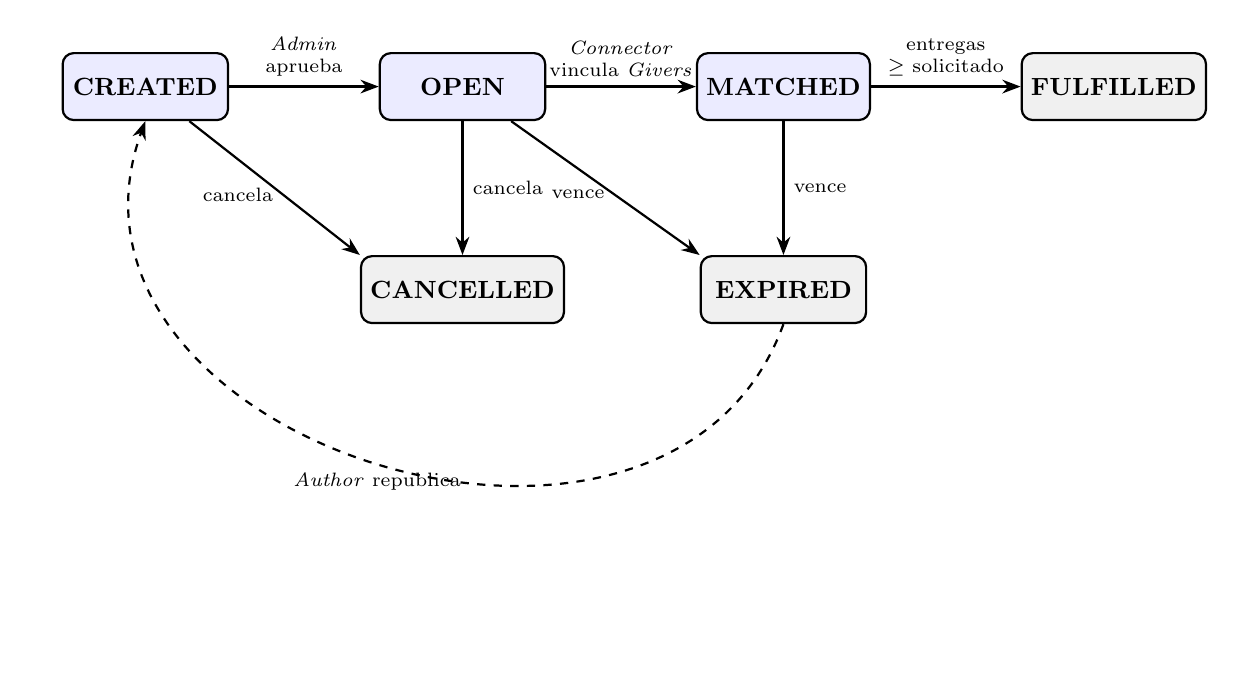
\begin{tikzpicture}[
  node distance=1.7cm and 1.9cm,
  state/.style={rectangle, rounded corners, draw=black, thick, fill=blue!8,
                minimum width=2.1cm, minimum height=0.85cm, align=center, font=\small\bfseries},
  terminal/.style={rectangle, rounded corners, draw=black, thick, fill=gray!12,
                minimum width=2.1cm, minimum height=0.85cm, align=center, font=\small\bfseries},
  trans/.style={-{Stealth}, thick},
  lbl/.style={font=\scriptsize, align=center}
]
  \node[state] (created) {CREATED};
  \node[state, right=of created] (open) {OPEN};
  \node[state, right=of open] (matched) {MATCHED};
  \node[terminal, right=of matched] (fulfilled) {FULFILLED};

  \node[terminal, below=of open] (cancelled) {CANCELLED};
  \node[terminal, below=of matched] (expired) {EXPIRED};

  \draw[trans] (created) -- node[lbl, above]{\textit{Admin}\\aprueba} (open);
  \draw[trans] (open) -- node[lbl, above]{\textit{Connector}\\vincula \textit{Givers}} (matched);
  \draw[trans] (matched) -- node[lbl, above]{entregas\\$\geq$ solicitado} (fulfilled);

  \draw[trans] (created) -- node[lbl, left, pos=0.55]{cancela} (cancelled.north west);
  \draw[trans] (open) -- node[lbl, right]{cancela} (cancelled);
  \draw[trans] (open) -- node[lbl, left, pos=0.55]{vence} (expired.north west);
  \draw[trans] (matched) -- node[lbl, right]{vence} (expired);

  \draw[trans, dashed] (expired.south) to[out=-110, in=-110, looseness=1.3]
        node[lbl, below, pos=0.5]{\textit{Author} republica} (created.south);
\end{tikzpicture}
\caption[Máquina de estados de la petición]{Máquina de estados de la petición.}
\label{fig:maquina-estados}
\end{figure}

El camino habitual de una petición es directo: nace en \textit{CREATED}, el administrador la valida y pasa a \textit{OPEN}, el conector le vincula donantes y avanza a \textit{MATCHED}, y solo cuando la ayuda entregada alcanza la solicitada se da por completada en \textit{FULFILLED}. De este camino se desvían dos finales alternativos. El primero, \textit{CANCELLED}, es una salida manual disponible mientras la petición sigue viva, en la que puede registrarse un motivo de cancelación para preservar la trazabilidad. El segundo, \textit{EXPIRED}, lo asigna en exclusiva un proceso programado cuando la fecha límite de una petición \textit{OPEN} o \textit{MATCHED} ha vencido; a diferencia del resto, no es un final definitivo, ya que el autor puede descartarla —con lo que pasa a \textit{CANCELLED}— o republicarla. Conviene precisar que republicar no reabre la misma petición, sino que genera una nueva al inicio del ciclo, copiando los datos y recalculando la cantidad pendiente. La Tabla~\ref{tab:transiciones} recoge de forma exhaustiva las transiciones admitidas, el evento que las dispara y el actor responsable.

\begin{table}[ht]
\centering
\caption[Transiciones de la máquina de estados]{Transiciones de la máquina de estados.}
\label{tab:transiciones}
\footnotesize
\renewcommand{\arraystretch}{1.3}
\begin{tabularx}{\textwidth}{%
  >{\raggedright\arraybackslash}p{2.5cm}%
  >{\raggedright\arraybackslash}p{2.3cm}%
  >{\raggedright\arraybackslash}X%
  >{\raggedright\arraybackslash}p{2.2cm}}
\toprule
\textbf{Origen} & \textbf{Destino} & \textbf{Evento} & \textbf{Responsable} \\
\midrule
\textit{CREATED} & \textit{OPEN} & Aprobación de la petición & \textit{Admin} / \textit{Author} \\
\textit{CREATED} & \textit{CANCELLED} & Rechazo antes de publicar & \textit{Admin} / \textit{Author} \\
\textit{OPEN} & \textit{MATCHED} & Vinculación de \textit{Givers} & \textit{Connector} \\
\textit{OPEN} & \textit{CANCELLED} & Cancelación manual & \textit{Admin} / \textit{Author} \\
\textit{OPEN} & \textit{EXPIRED} & Vencimiento de la fecha límite & Proceso automático \\
\textit{MATCHED} & \textit{FULFILLED} & Entregas acumuladas $\geq$ lo solicitado, o cierre manual anticipado & Sistema / \textit{Connector} \\
\textit{MATCHED} & \textit{CANCELLED} & Cancelación manual & \textit{Admin} / \textit{Author} \\
\textit{MATCHED} & \textit{EXPIRED} & Vencimiento de la fecha límite & Proceso automático \\
\textit{EXPIRED} & \textit{CANCELLED} & Descarte de la petición caducada & \textit{Admin} / \textit{Author} \\
\textit{EXPIRED} & \textit{CREATED} & Republicación (genera una nueva petición) & \textit{Author} \\
\bottomrule
\end{tabularx}

\vspace{0.4em}
{\footnotesize La columna «Responsable» indica el rol que habitualmente ejecuta cada transición. La capa de servicio valida qué cambios de estado son \textit{estructuralmente} posibles, mientras que la autorización sobre \textit{qué} rol puede invocarlos recae en los \textit{middlewares} de rol del \textit{endpoint} correspondiente (véase el Capítulo 6); el rol \textit{Admin} dispone además de paso franco sobre la máquina de estados.}
\end{table}

\subsection{Reglas de negocio e invariantes}

Más allá de las transiciones de estado, el diseño debe garantizar un conjunto de invariantes: propiedades que el sistema mantiene siempre, con independencia de quién opere o en qué orden. Recogerlas de forma sistemática en esta fase evita que se diluyan entre el código y permite verificarlas después durante las pruebas. La Tabla~\ref{tab:invariantes} las consolida. El énfasis aquí está en \textit{qué} se garantiza; la mecánica concreta con que cada invariante se hace cumplir en el servidor se aborda en el Capítulo 6.

\begin{table}[ht]
\centering
\caption[Invariantes de diseño del sistema]{Invariantes de diseño del sistema.}
\label{tab:invariantes}
\footnotesize
\renewcommand{\arraystretch}{1.3}
\begin{tabularx}{\textwidth}{%
  >{\raggedright\arraybackslash}p{2.4cm}%
  >{\raggedright\arraybackslash}X}
\toprule
\textbf{Invariante} & \textbf{Garantía de diseño} \\
\midrule
Control de sobredonación & La suma de las entregas registradas nunca puede superar la cantidad solicitada; el sistema rechaza cualquier entrega que exceda lo pendiente. \\
Cierre automático & Cuando lo entregado iguala o supera lo solicitado, la petición transita a \textit{FULFILLED} sin intervención manual adicional. \\
Autoría no falsificable & La autoría de una petición o entrega se deriva siempre de la identidad del \textit{token} de sesión, ignorando cualquier identificador que llegue en el cuerpo de la solicitud. \\
Aislamiento por consulta & Cada usuario solo recibe los registros que le competen según su rol y especialidad, filtrados en el propio acceso a datos y no en la presentación. \\
Especialidad obligatoria & Los roles de experto (\textit{Connector} y \textit{Giver}) deben tener al menos un dominio de especialidad asociado para poder operar sobre peticiones de ese ámbito. \\
Baja lógica & La eliminación de usuarios nunca es física: se marca el registro como inactivo para preservar la trazabilidad histórica de las intervenciones. \\
\bottomrule
\end{tabularx}
\end{table}

\subsection{Decisiones de diseño transversales}

Durante el diseño surgieron varias decisiones que no encajan en una única capa, sino que atraviesan el sistema y afectan directamente a la experiencia de los usuarios. Se recogen aquí porque, pese a su carácter puntual, condicionan de forma apreciable cómo se opera la plataforma.

\textbf{Notificación en el emparejamiento.} Cuando un conector vincula donantes a una petición, el sistema contempla el envío de una notificación por correo a las partes implicadas. La decisión de diseño relevante es desacoplar esta acción del flujo principal: el emparejamiento se confirma con independencia de que la notificación se entregue, de modo que un fallo en el servicio de correo nunca bloquea la operación de negocio.

\textbf{Filtrado de donantes por dominio.} En el momento de emparejar, la interfaz no ofrece al conector la lista completa de donantes, sino únicamente aquellos cuya especialidad coincide con el dominio de la petición. Esta restricción, distinta del filtrado de privacidad de las peticiones, persigue un objetivo de usabilidad: reducir el espacio de decisión del conector y orientarlo hacia los donantes pertinentes, disminuyendo el riesgo de emparejamientos poco adecuados.

\textbf{Imagen en las Historias de Impacto.} El diseño de la Historia de Impacto prevé acompañar el texto generado con una imagen representativa. Se trata de una decisión orientada a la comunicación: una narrativa visual resulta más eficaz para atraer colaboradores que un bloque de texto, en línea con el papel que el propio modelo AskingX atribuye a las historias de éxito.

\textbf{Gestión de especialidades por el administrador.} La relación de muchos a muchos entre usuarios expertos y dominios no es estática. El diseño reserva al administrador la capacidad de editar las especialidades de cada experto, de modo que la asignación de dominios pueda ajustarse a medida que evoluciona el perfil de los conectores y donantes, sin necesidad de recrear sus cuentas.

\subsection{Diseño de la interfaz}

El diseño de la interfaz parte de los principios ya fijados —enfoque \textit{mobile-first} y aplicación de página única— y los concreta en un conjunto de vistas adaptadas a cada rol. La Figura~\ref{fig:mockups} muestra las pantallas principales de la plataforma.

\begin{figure}[htbp]
\centering
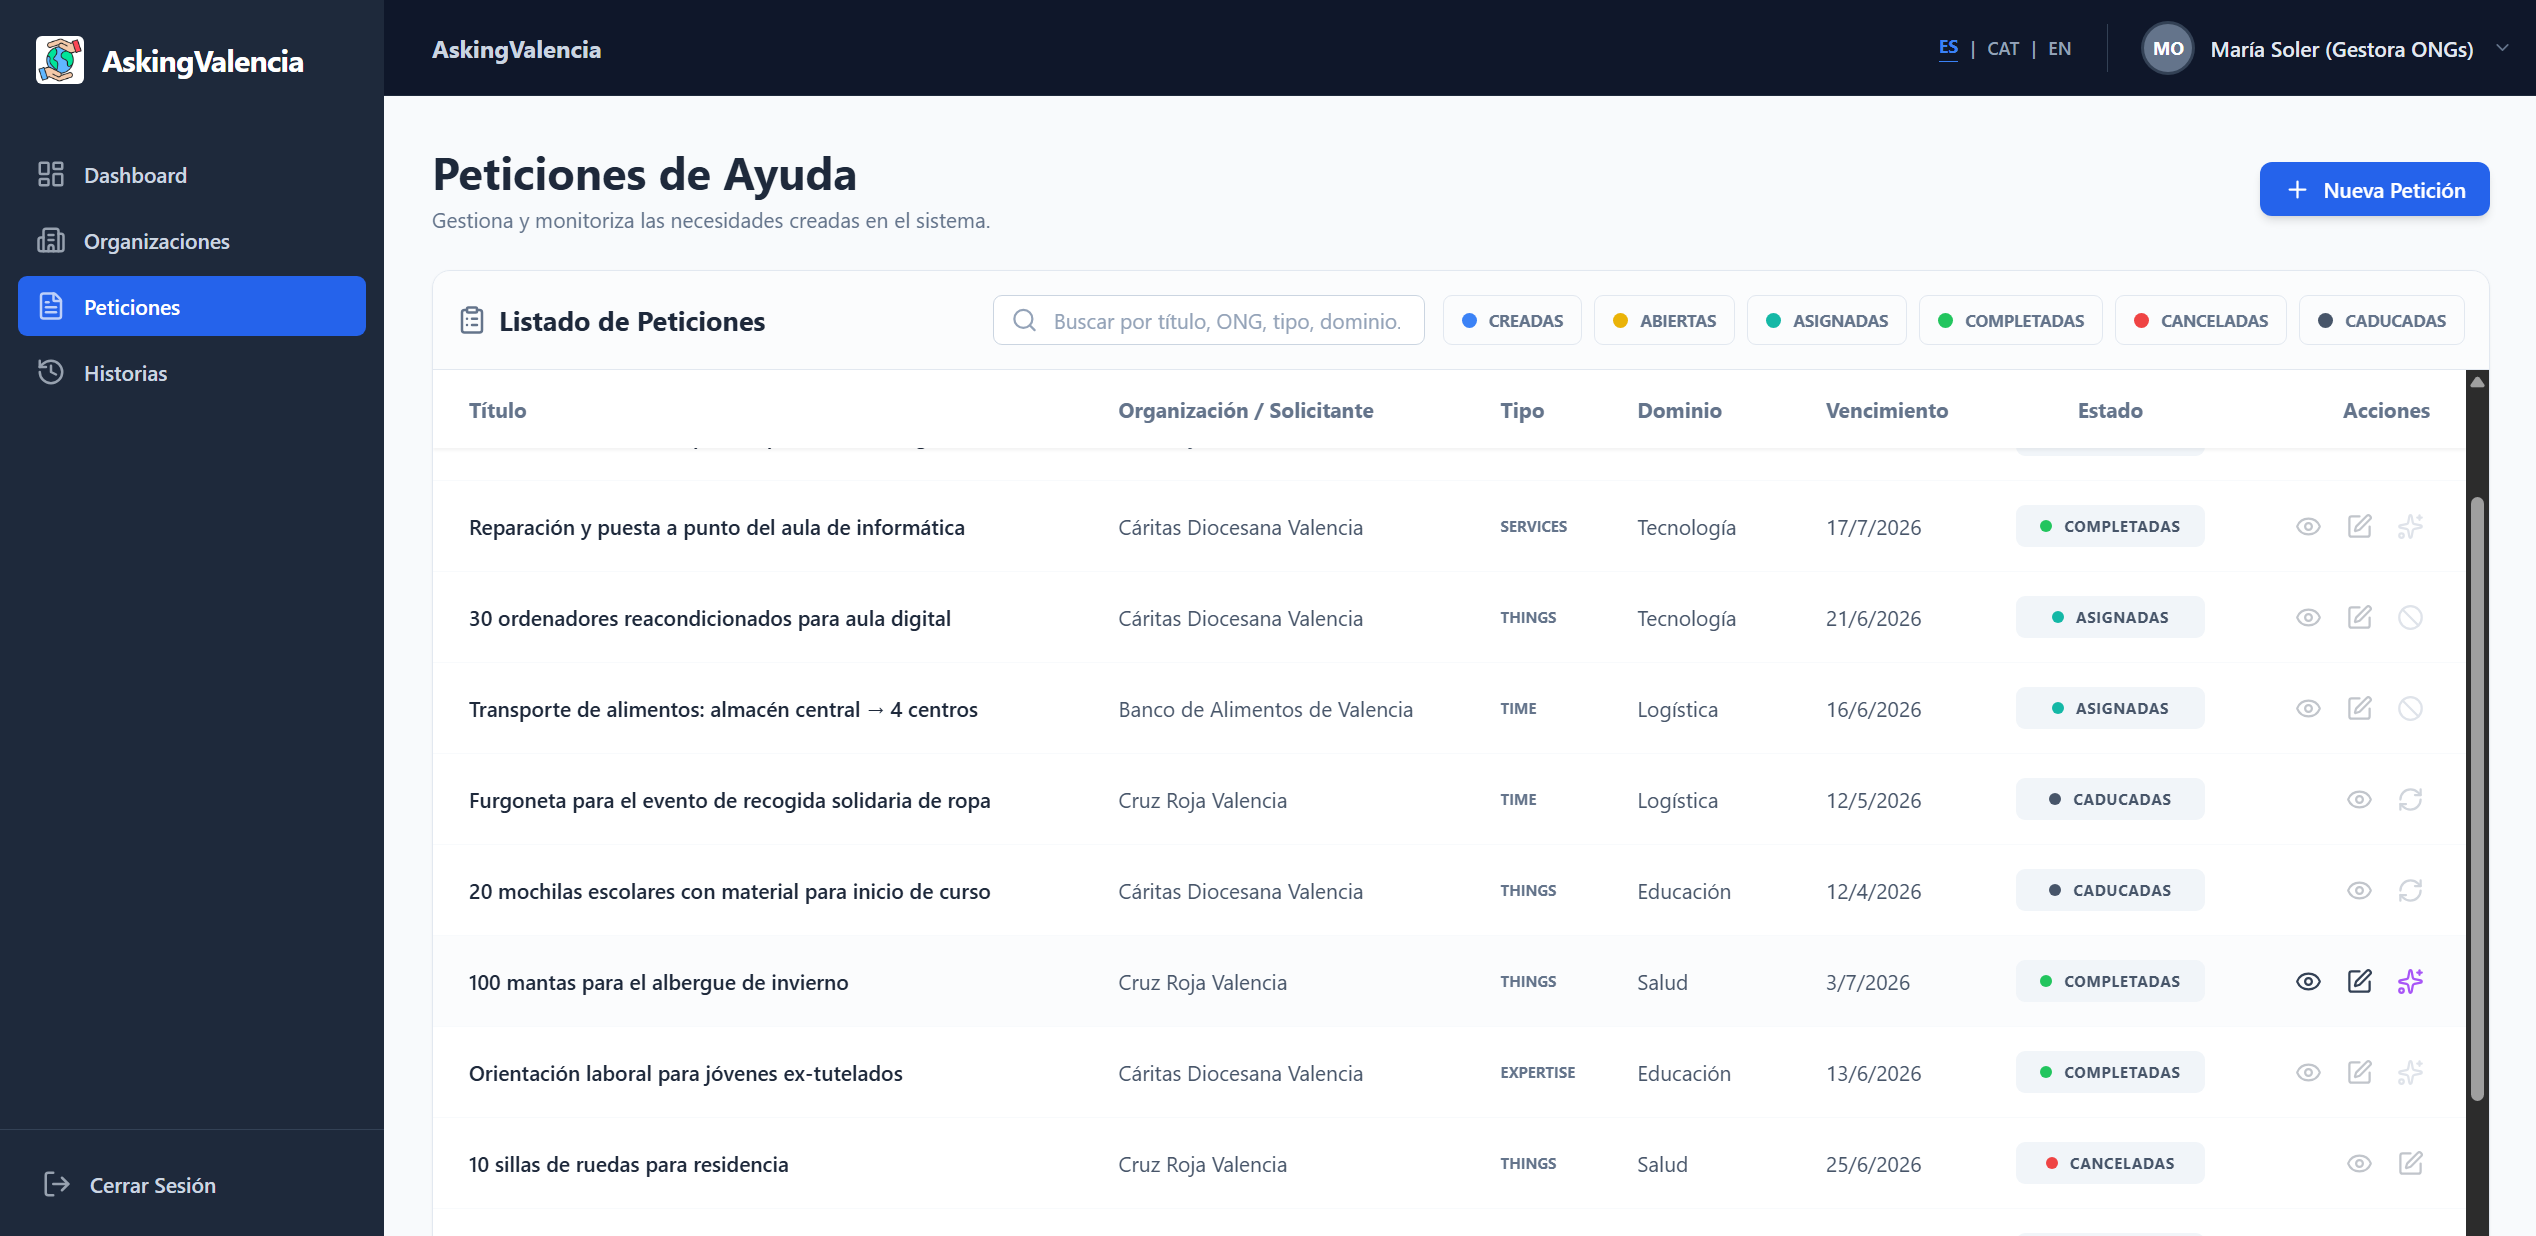
\includegraphics[width=\textwidth]{mockups}
\caption[Panel de peticiones del \textit{AskAuthor}]{Panel de peticiones del rol \textit{AskAuthor}.}
\label{fig:mockups}
\end{figure}

El diseño visual se rige por dos criterios. El primero es el \textbf{renderizado según el rol}: cada usuario accede a un conjunto reducido de vistas y acciones, las pertinentes a sus competencias, lo que disminuye la carga cognitiva y refuerza el aislamiento de los flujos de trabajo. El segundo atiende a un problema recurrente en interfaces densas en menús y diálogos: la \textbf{superposición de elementos flotantes}. Los modales y los menús desplegables se resuelven renderizándolos de forma condicional sobre una capa a pantalla completa, posicionada de forma fija y superpuesta al resto de la interfaz, cuyo orden de apilamiento se gobierna de manera explícita y jerárquica para que un diálogo abierto sobre otro quede siempre por encima. El detalle de cómo se materializan estos componentes en \textit{React} se aborda en el capítulo siguiente.

\chapter{Desarrollo de la solución propuesta}

El capítulo anterior fijó \textit{qué} se diseñó: la arquitectura por capas, el modelo de datos, la máquina de estados y las invariantes que el sistema debe garantizar. Este capítulo desciende al \textit{cómo}, es decir, a la materialización de esas decisiones en código. Para no reiterar lo ya expuesto, las justificaciones de diseño se dan por sentadas y la exposición se centra en los mecanismos concretos de implementación, apoyándose en fragmentos reales del código del proyecto cuando aportan claridad. Se recorren, en este orden, la organización del servidor en capas, el desarrollo del \textit{backend} y la persistencia, la construcción del cliente web, la integración del servicio de Inteligencia Artificial y, por último, la gestión del flujo relacional uno a varios que vertebra las entregas de ayuda.

\section{Separación por capas lógicas}

La organización del servidor traslada de forma literal la arquitectura por capas descrita en el Capítulo 5 a la estructura de directorios del proyecto. Cada responsabilidad reside en su propia carpeta dentro de \texttt{backend/src}: las rutas (\texttt{routes/}) declaran los \textit{endpoints}, los controladores (\texttt{controllers/}) validan la entrada y traducen entre HTTP y dominio, los servicios (\texttt{services/}) concentran la lógica de negocio y el acceso a datos vía \textit{Prisma}, y los \textit{middlewares} (\texttt{middlewares/}) interceptan de forma transversal la autenticación, el control de acceso y el tratamiento de errores. Esta correspondencia uno a uno entre concepto y carpeta no es meramente estética: permite localizar cualquier pieza por su responsabilidad y, sobre todo, mantener los controladores delgados, delegando en la capa de servicios todo aquello que tenga peso de negocio.

El recorrido de una petición HTTP ilustra cómo colaboran las capas. La Figura~\ref{fig:flujo-capas} representa ese trayecto. La solicitud entra por una ruta, que la encadena a través de los \textit{middlewares} de autenticación y de rol; si los supera, alcanza el controlador, que valida el cuerpo con \textit{Zod} y, solo entonces, invoca al servicio correspondiente; este ejecuta la lógica y dialoga con la base de datos mediante \textit{Prisma}. La respuesta deshace el camino. Cualquier error lanzado en el trayecto —de validación, de autorización o de negocio— se desvía mediante \texttt{next(error)} hacia un único \textit{middleware} de errores, que centraliza la conversión a una respuesta HTTP coherente.

\begin{figure}[htbp]
\centering
\begin{tikzpicture}[
  node distance=0.7cm and 1.0cm,
  capa/.style={rectangle, rounded corners, draw=black, thick, fill=blue!8,
               minimum width=2.05cm, minimum height=1.0cm, align=center, font=\scriptsize},
  store/.style={rectangle, rounded corners, draw=black, thick, fill=gray!12,
               minimum width=2.05cm, minimum height=1.0cm, align=center, font=\scriptsize},
  err/.style={rectangle, rounded corners, draw=black!60, thick, fill=red!8,
               minimum width=2.05cm, minimum height=1.0cm, align=center, font=\scriptsize},
  fl/.style={-{Stealth}, thick},
  lbl/.style={font=\tiny, align=center}
]
  \node[capa] (ruta) {Ruta\\\textit{+ middlewares}};
  \node[capa, right=of ruta] (ctrl) {Controlador\\\textit{(Zod)}};
  \node[capa, right=of ctrl] (svc) {Servicio\\\textit{(negocio)}};
  \node[store, right=of svc] (db) {\textit{Prisma}\\PostgreSQL};
  \node[err, below=1.1cm of ctrl] (errh) {\textit{Error\\Handler}};

  \draw[fl] (ruta) -- node[lbl, above]{HTTP} (ctrl);
  \draw[fl] (ctrl) -- node[lbl, above]{datos\\validados} (svc);
  \draw[fl] (svc) -- node[lbl, above]{consulta} (db);
  \draw[fl, dashed] (db) to[bend left=18] node[lbl, below]{resultado} (svc);

  \draw[fl, red!50!black] (ctrl) -- node[lbl, right]{\texttt{next(err)}} (errh);
  \draw[fl, red!50!black] (svc.south) to[out=-90, in=0] (errh.east);
  \draw[fl, red!50!black, dashed] (errh.west) to[out=180, in=-90] node[lbl, left]{HTTP 4xx/5xx} (ruta.south);
\end{tikzpicture}
\caption[Recorrido de una petición a través de las capas]{Recorrido de una petición a través de las capas del servidor.}
\label{fig:flujo-capas}
\end{figure}

Ese gestor centralizado es la pieza que mantiene estable el servidor. En lugar de dispersar bloques \texttt{try/catch} con respuestas heterogéneas por cada controlador, todos los errores convergen en un único punto que discrimina su naturaleza: si se trata de un fallo de validación de \textit{Zod} se responde con un código 400 y el mensaje legible del esquema incumplido; en caso contrario se emplea el código de estado que el propio error transporta —o un 500 por defecto—. El Fragmento~\ref{lst:errorhandler} recoge esta lógica, que evita que una entrada malformada o un error operativo derriben el proceso de \textit{Node.js}.

\begin{figure}[htbp]
\begin{lstlisting}[caption={Gestor de errores centralizado que distingue los fallos de validación de \textit{Zod} del resto.}, label={lst:errorhandler}]
const errorHandler = (err, req, res, next) => {
  if (err instanceof ZodError) {
    const mensajes = err.issues.map(issue => issue.message);
    return res.status(400).json({ success: false, message: mensajes[0] });
  }
  const statusCode = err.statusCode || 500;
  res.status(statusCode).json({ success: false, message: err.message });
};
\end{lstlisting}
\end{figure}

La capa de rutas expone una API REST cuyos puntos de entrada se organizan por recurso. La Tabla~\ref{tab:endpoints} resume los principales, junto con el rol al que se restringe cada uno.

\begin{table}[ht]
\centering
\caption[Principales endpoints de la API REST]{Principales \textit{endpoints} de la API REST.}
\label{tab:endpoints}
\footnotesize
\renewcommand{\arraystretch}{1.2}
\begin{tabularx}{\textwidth}{%
  >{\raggedright\arraybackslash}p{1.1cm}%
  >{\raggedright\arraybackslash}p{4.0cm}%
  >{\raggedright\arraybackslash}p{2.9cm}%
  >{\raggedright\arraybackslash}X}
\toprule
\textbf{Método} & \textbf{Ruta} & \textbf{Rol} & \textbf{Función} \\
\midrule
\texttt{POST}   & \texttt{/api/users/login}        & Pública                                                & Autenticar y emitir el \textit{token} \\
\texttt{POST}   & \texttt{/api/users/register}     & \textit{Admin}                                         & Alta de personal interno \\
\texttt{GET}    & \texttt{/api/users}              & \textit{Admin}                                         & Listar usuarios \\
\texttt{PATCH}  & \texttt{/api/users/:id}          & \textit{Admin}                                         & Editar usuario (estado, especialidades) \\
\texttt{PATCH}  & \texttt{/api/users/profile}      & Autenticado                                            & Editar el perfil propio (idioma, nombre) \\
\midrule
\texttt{POST}   & \texttt{/api/askers}             & \textit{Author}                                        & Registrar una entidad solicitante \\
\texttt{GET}    & \texttt{/api/askers/author/:id}  & Autenticado                                            & Listar las entidades de un autor \\
\texttt{DELETE} & \texttt{/api/askers/:id}         & \textit{Author} / \textit{Admin}                       & Eliminar una entidad \\
\midrule
\texttt{GET}    & \texttt{/api/asks}               & Autenticado                                            & Listar peticiones (filtradas por rol) \\
\texttt{POST}   & \texttt{/api/asks}               & \textit{Author}                                        & Crear una petición (nace en \textit{CREATED}) \\
\texttt{PUT}    & \texttt{/api/asks/:id}           & \textit{Author} / \textit{Admin}                       & Editar una petición \\
\texttt{PATCH}  & \texttt{/api/asks/:id/status}    & \textit{Author} / \textit{Admin} / \textit{Connector}  & Cambiar el estado \\
\texttt{PATCH}  & \texttt{/api/asks/:id/match}     & \textit{Connector}                                     & Vincular donantes \\
\texttt{PUT}    & \texttt{/api/asks/:id/discard}   & \textit{Author} / \textit{Admin}                       & Descartar una petición caducada \\
\texttt{POST}   & \texttt{/api/asks/:id/republish} & \textit{Author} / \textit{Admin}                       & Republicar una petición caducada \\
\midrule
\texttt{POST}   & \texttt{/api/fulfillments}       & \textit{Connector} / \textit{Author}                   & Registrar una entrega \\
\midrule
\texttt{GET}    & \texttt{/api/stories}                 & Autenticado                                       & Listar historias (filtradas por rol) \\
\texttt{POST}   & \texttt{/api/stories/}\newline\texttt{generate/:askId} & \textit{Author} / \textit{Admin}                  & Generar la historia con IA \\
\texttt{PATCH}  & \texttt{/api/stories/:id}             & \textit{Author} / \textit{Admin}                  & Editar o publicar una historia \\
\midrule
\texttt{GET}    & \texttt{/api/domains}            & Pública                                                & Listar dominios temáticos \\
\texttt{POST}   & \texttt{/api/domains}            & \textit{Admin}                                         & Crear un dominio \\
\texttt{PATCH}  & \texttt{/api/domains/:id}        & \textit{Admin}                                         & Activar o editar un dominio \\
\midrule
\texttt{GET}    & \texttt{/api/stats/summary}      & \textit{Admin}                                         & Métricas del cuadro de mandos \\
\texttt{GET}    & \texttt{/api/config}             & Pública                                                & Leer la configuración de la instancia \\
\texttt{PUT}    & \texttt{/api/config}             & \textit{Admin}                                         & Editar la configuración global \\
\bottomrule
\end{tabularx}

\vspace{0.4em}
{\footnotesize Todas las rutas salvo las marcadas como «Pública» exigen un \textit{token} válido. El rol \textit{Admin} dispone de paso franco y puede invocar cualquier \textit{endpoint}, con independencia del rol indicado en la tabla.}
\end{table}

\section{Desarrollo del Backend y persistencia de datos}

\subsection{Prisma como puente entre el modelo y la base de datos}

La persistencia se apoya íntegramente en \textit{Prisma}, que actúa como puente entre el modelo de clases del Capítulo 5 y las tablas físicas de PostgreSQL. El fichero \texttt{schema.prisma} es la única fuente de verdad: en él se declaran las entidades, sus atributos y las relaciones, y a partir de él se genera un cliente fuertemente tipado y se derivan las migraciones que crean el esquema en la base de datos. La herencia de tabla única descrita en el diseño se traduce aquí en una sola tabla \texttt{Ask} con los campos especializados (\texttt{quantityRequested}, \texttt{estimatedHours}, \texttt{requiredSkill} y \texttt{serviceLocation}) declarados como opcionales; al crear una petición solo se rellena el campo que corresponde a su tipo, y los demás permanecen nulos.

El acceso a los datos no emplea SQL directo, sino las operaciones del cliente generado. A lo largo del servicio se usan las primitivas habituales —\texttt{findUnique} para recuperar por identificador, \texttt{create} y \texttt{update} para altas y modificaciones, \texttt{findMany} para listados filtrados— junto con otras de mayor calado que se detallan más adelante: \texttt{aggregate} para sumar entregas, \texttt{updateMany} para la caducidad masiva y \texttt{\$transaction} para garantizar atomicidad. Las relaciones se manipulan de forma declarativa mediante \texttt{connect} y \texttt{set}, lo que evita gestionar a mano las tablas intermedias.

\subsection{Autenticación y control de acceso}

La gestión de identidad concreta lo anunciado en el diseño. En el alta de un usuario, la contraseña nunca se almacena en claro: se cifra con \textit{bcrypt} aplicando un factor de coste de diez rondas de sal antes de persistirla. En el inicio de sesión, el servicio recupera al usuario, comprueba que esté activo —un usuario dado de baja lógica no puede autenticarse—, contrasta la contraseña con \texttt{bcrypt.compare} y, si todo es correcto, emite un \textit{JSON Web Token} \cite{jwt_rfc} firmado con una vigencia de veinticuatro horas. El \textit{token} transporta en su carga útil únicamente el identificador y el rol del usuario, lo justo para resolver la autorización en las peticiones siguientes sin necesidad de consultar la base de datos en cada llamada.

Sobre esa base operan dos \textit{middlewares} encadenados. El primero verifica criptográficamente el \textit{token} recibido en la cabecera \texttt{Authorization} con formato \texttt{Bearer}, y si es válido inyecta los datos del usuario en el objeto de la petición; si está ausente, malformado o caducado, responde con un 401 sin propagar la excepción al hilo principal. El segundo recibe la lista de roles autorizados para cada ruta y bloquea con un 403 a quien no figure en ella, con una salvedad deliberada: el rol \textit{Admin} dispone de un paso franco (\textit{by-pass}) que le concede acceso global, materializando el «modo administrador» previsto en el modelo de permisos.

La garantía de autoría no falsificable enunciada entre las invariantes de la Tabla~\ref{tab:invariantes} se resuelve en el controlador de creación de peticiones. Antes de validar el cuerpo entrante, el controlador \textbf{sobrescribe} el identificador del autor con el que viaja firmado en el \textit{token}, de modo que cualquier intento de suplantación enviado por el cliente se descarta de raíz:

\begin{figure}[htbp]
\begin{lstlisting}[caption={Asignación de la autoría a partir del token, descartando el identificador que enviase el cliente.}, label={lst:antispoofing}]
const createAskController = async (req, res, next) => {
  req.body.askAuthorId = req.user.userId;        // autoria tomada del token
  const validatedData = createAskSchema.parse(req.body);
  const ask = await askService.createAsk(validatedData);
  res.status(201).json({ success: true, data: ask });
};
\end{lstlisting}
\end{figure}

\subsection{La máquina de estados en el servicio}

La máquina de estados que la Figura~\ref{fig:maquina-estados} presentó como artefacto de diseño se hace cumplir en la capa de servicio mediante una tabla de transiciones explícita. Cuando se solicita un cambio de estado, el servicio consulta qué destinos son válidos desde el estado actual y rechaza con un 400 cualquier salto no contemplado, impidiendo así que un error del cliente lleve a una petición de \textit{CREATED} a \textit{FULFILLED} de un solo paso. El Fragmento~\ref{lst:statemachine} muestra esta validación. Conviene distinguir dos planos que no deben confundirse: esta tabla decide qué transiciones son \textit{estructuralmente} posibles, mientras que la autorización sobre \textit{quién} puede provocarlas recae en los \textit{middlewares} de rol descritos antes. El rol \textit{Admin} queda exento de la comprobación estructural, por las mismas razones operativas que en el resto del sistema.

\begin{figure}[htbp]
\begin{lstlisting}[caption={Tabla de transiciones que materializa la máquina de estados en la capa de servicio.}, label={lst:statemachine}]
const validTransitions = {
  CREATED:   ['OPEN', 'CANCELLED'],
  OPEN:      ['MATCHED', 'CANCELLED', 'CREATED'],
  MATCHED:   ['FULFILLED', 'OPEN', 'CANCELLED'],
  FULFILLED: [], CANCELLED: [], EXPIRED: []   // estados terminales
};
const allowed = validTransitions[current] || [];
if (!allowed.includes(target) && current !== target) {
  const error = new Error(`Transicion no permitida: de ${current} a ${target}.`);
  error.statusCode = 400;
  throw error;
}
\end{lstlisting}
\end{figure}

Esta misma operación encierra un detalle de coherencia: al revertir una petición al estado \textit{CREATED} se deshace su asignación, vaciando la lista de donantes y el conector responsable, de modo que el retroceso devuelve la petición a un punto de partida limpio en lugar de dejar referencias colgantes.

\subsection{Filtrado de visibilidad a nivel de consulta}

El aislamiento por consulta, otra de las invariantes de diseño, se implementa construyendo dinámicamente la cláusula de filtrado de \textit{Prisma} según el rol de quien consulta, en lugar de recuperar todas las peticiones y descartarlas después en la capa de presentación. Filtrar en el propio acceso a datos es más seguro —la información que no corresponde a un usuario nunca llega a salir de la base de datos— y más eficiente. Cada rol determina una forma distinta del filtro: el \textit{Admin} no recibe restricción alguna; el \textit{AskAuthor} queda limitado a las peticiones de las que es autor; el \textit{Giver} solo ve aquellas en las que participa o ha colaborado; y el \textit{Connector} recibe la combinación de su «bolsa de trabajo» —peticiones abiertas que coinciden con sus dominios de especialidad, obtenidos en una consulta previa— y los casos que él mismo gestiona. Este último filtro ejemplifica la lógica condicional que se traslada a la consulta:

\begin{figure}[htbp]
\begin{lstlisting}[caption={Construcción del filtro de visibilidad del \textit{Connector} sobre la consulta de \textit{Prisma}.}, label={lst:visibilidad}]
query.where.OR = [
  { status: 'OPEN', domainId: { in: specialtyIds } }, // bolsa de trabajo
  { connectorId: user.userId }                         // casos propios
];
\end{lstlisting}
\end{figure}

\section{Desarrollo del Frontend}

\subsection{Estructura de la aplicación de página única}

El cliente se inicializa en \texttt{main.jsx}, donde la aplicación se envuelve en el enrutador y en el modo estricto de \textit{React}, y se monta sobre ella el proveedor de idioma que se describe más adelante. El árbol de rutas vive en \texttt{App.jsx}, que separa la ruta pública de acceso del resto, agrupadas estas bajo un componente de ruta protegida que verifica la sesión antes de ceder el paso. Las vistas autenticadas comparten un \textit{layout} maestro que aloja la barra lateral y la superior y reserva el área central, mediante un \textit{outlet}, para la página activa. De este modo la navegación entre secciones no recarga la página: solo se sustituye el contenido del área central, en coherencia con el modelo de aplicación de página única.

Toda la comunicación con el servidor se concentra en una capa de servicios independiente de los componentes visuales, construida sobre la API nativa \textit{Fetch} sin librerías de terceros. Cada módulo de servicio inyecta de forma uniforme el \textit{token} de sesión, recuperado del almacenamiento local del navegador, en la cabecera de autorización de cada llamada. Aislar así la comunicación cumple el principio de separación de responsabilidades: si un \textit{endpoint} cambia, la modificación se circunscribe al servicio correspondiente y no se propaga a las vistas. A esta disciplina se añade una programación defensiva en el lado del cliente, que valida la forma de las respuestas —comprobando, por ejemplo, que un dato es realmente un \textit{array} antes de recorrerlo— para que una respuesta inesperada del servidor degrade la experiencia con elegancia en lugar de provocar una pantalla en blanco.

\subsection{Formularios polimórficos y gestión del estado}

La gestión del estado de la interfaz se resuelve con los \textit{hooks} estándar de \textit{React}: el estado local de formularios, cargas y modales, y los efectos que disparan las llamadas asíncronas en el momento en que un componente se monta o un modal se abre. El ejemplo más representativo de esta capa es el modal de creación de peticiones, diseñado para ser polimórfico en un doble sentido. Por un lado, el mismo componente sirve para crear y para editar, distinguiendo ambos modos según reciba o no una petición existente, lo que evita duplicar un formulario complejo. Por otro, su contenido muta según el tipo de petición elegido: al seleccionar «cosas» aparece el campo de cantidad, al elegir «tiempo» el de horas estimadas, y así sucesivamente, de manera que el formulario envía al servidor únicamente los campos pertinentes a cada tipo. Esta correspondencia entre la interfaz y la herencia de tabla única del modelo de datos garantiza que cliente y servidor compartan la misma noción de qué información define a cada tipo de petición.

Un detalle recurrente que mereció atención fue el tratamiento de las fechas de vencimiento. Para evitar el clásico desfase entre la hora local y el horario universal, el cálculo de la fecha mínima seleccionable se realiza con la zona horaria del navegador, bloqueando de forma nativa la elección de fechas pasadas, y el valor se normaliza al estándar ISO 8601 antes de enviarlo, asegurando su correcta interpretación por parte del servidor.

\subsection{Superposición de modales y menús desplegables}

Un problema recurrente en interfaces con muchos diálogos es que un modal o un menú quede oculto tras otro elemento por efecto del recorte o del orden de apilamiento de su contenedor. La solución adoptada renderiza estos componentes de forma condicional —solo existen en el árbol de la interfaz mientras están abiertos— sobre una capa a pantalla completa, posicionada de forma fija, que cubre toda la ventana y atenúa el fondo. El orden de apilamiento se gobierna de forma explícita mediante cotas crecientes: los diálogos de primer nivel ocupan una cota base, mientras que los que pueden abrirse encima de ellos —por ejemplo, el modal de una Historia de Impacto lanzado desde el detalle de una petición— reciben una cota superior, de modo que la jerarquía visual se mantiene siempre coherente. Esta estrategia, sencilla y predecible, evita introducir dependencias adicionales y mantiene cada modal autocontenido.

\subsection{Cuadro de mandos por rol}

La pantalla de inicio tras la autenticación es un cuadro de mandos que ofrece a cada usuario una visión sintética del estado del sistema dentro del ámbito de sus competencias. Un único componente actúa de enrutador y, según el rol, presenta una composición distinta de indicadores, en coherencia con el renderizado condicional descrito anteriormente. El administrador obtiene una panorámica global —número total de peticiones, entidades y dominios, junto con el reparto por estado—; el \textit{AskAuthor}, los datos de las entidades y peticiones que gestiona; el \textit{Connector}, el recuento de peticiones abiertas, asignadas y completadas; y el \textit{Giver}, el resumen de sus colaboraciones asignadas y completadas.

Cada indicador se presenta como una tarjeta de métrica reutilizable, y la distribución de las peticiones por estado se visualiza mediante un gráfico circular generado con la biblioteca \textit{Chart.js}\footnote{\url{https://www.chartjs.org/docs/}}. Un aspecto relevante para la coherencia del sistema es que los indicadores se derivan de los mismos datos que el resto de la aplicación ya consume —el listado de peticiones filtrado por rol en el servidor—, de modo que el cuadro de mandos refleja exactamente la información que cada perfil está autorizado a ver, sin abrir una vía de acceso distinta a la descrita en el aislamiento por consulta. La Figura~\ref{fig:dashboard} muestra el cuadro de mandos del administrador.

\begin{figure}[htbp]
\centering
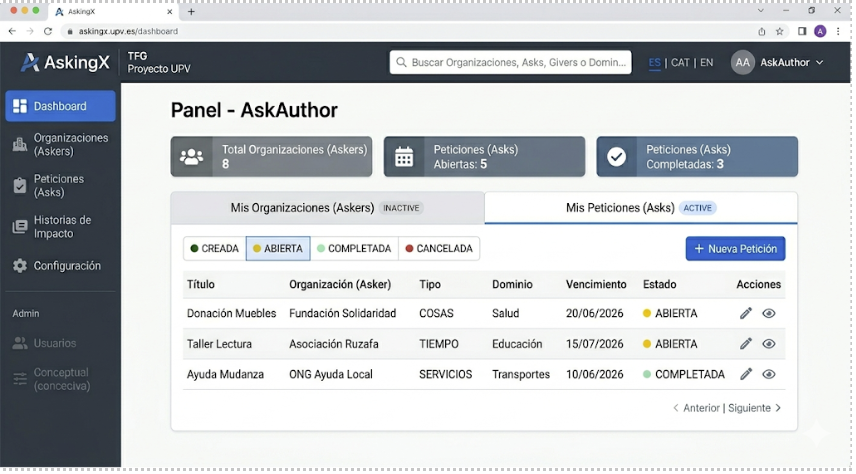
\includegraphics[width=\textwidth]{dashboard}
\caption[Cuadro de mandos del administrador]{Cuadro de mandos del administrador.}
\label{fig:dashboard}
\end{figure}

\subsection{El tablero del Connector}

La vista de mayor riqueza interactiva es el tablero del \textit{Connector}, que organiza las peticiones en columnas según su estado y permite arrastrar las tarjetas entre ellas empleando la API nativa de arrastrar y soltar de HTML5. Cada vez que una tarjeta se suelta en una columna distinta, el componente despacha la llamada correspondiente a la capa de servicios para asignar donantes o cambiar el estado de la petición, y actualiza el tablero en consecuencia. La Figura~\ref{fig:kanban} muestra esta vista.

\begin{figure}[htbp]
\centering
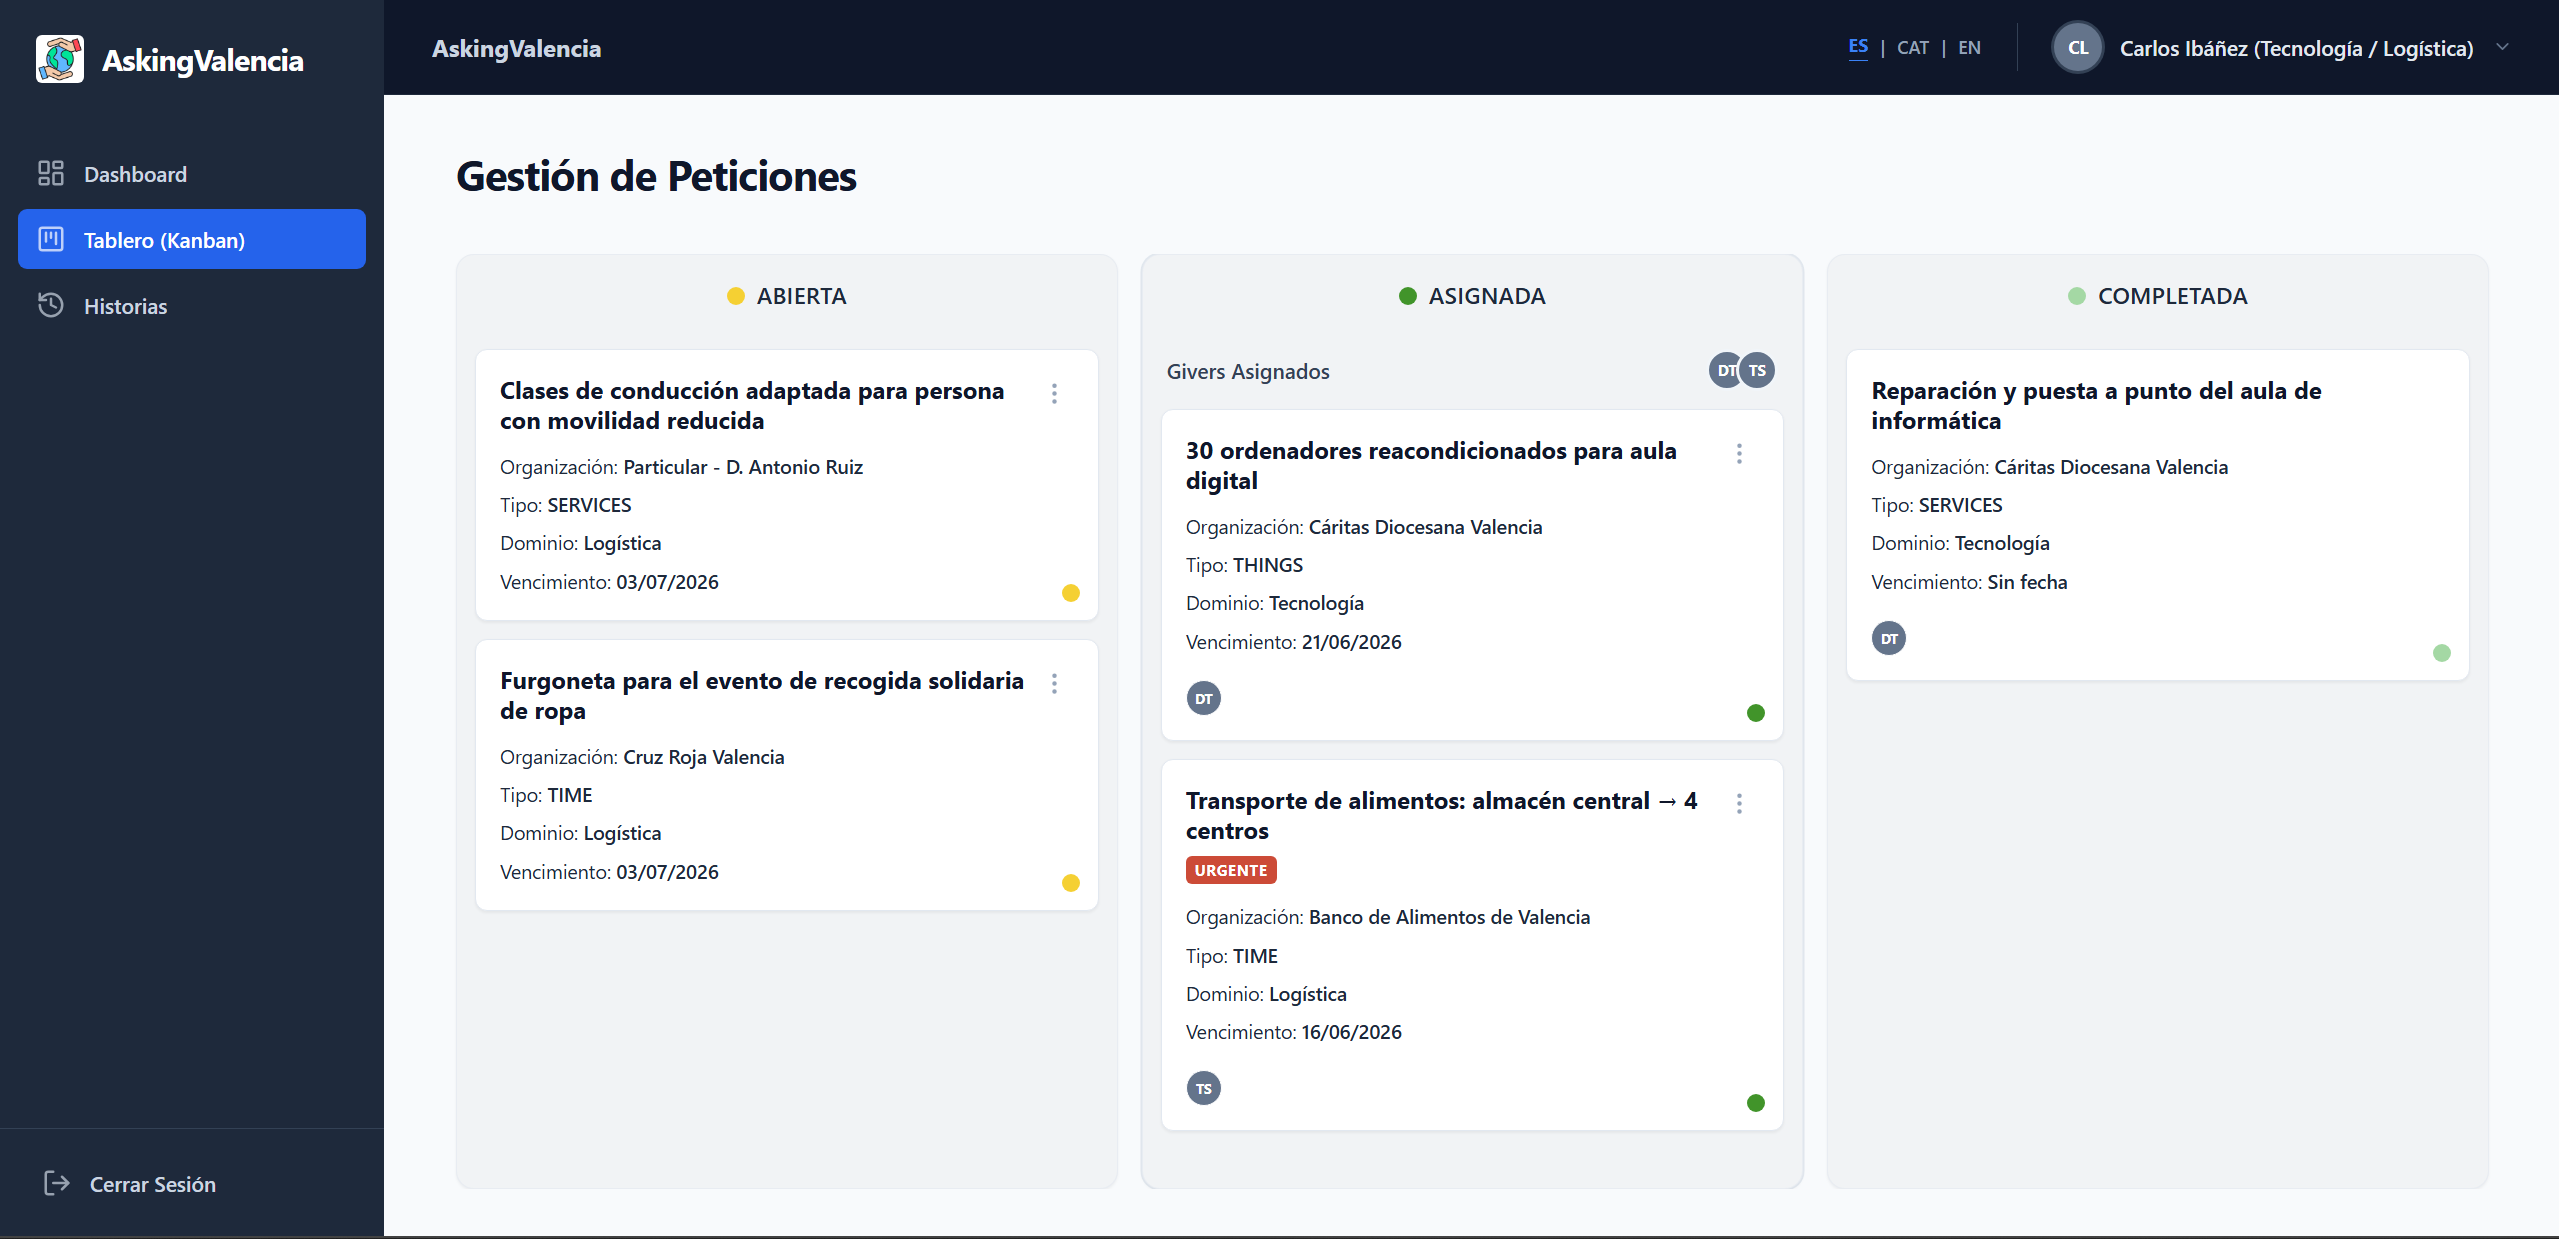
\includegraphics[width=\textwidth]{kanban}
\caption[Tablero del Connector]{Tablero del \textit{Connector}.}
\label{fig:kanban}
\end{figure}

\subsection{Internacionalización de la interfaz}

El soporte multilingüe exigido por los requisitos se ha implementado sin recurrir a librerías externas, mediante un patrón ligero de diccionarios. Un único fichero reúne, para cada uno de los tres idiomas —español, valenciano e inglés—, el mismo conjunto de claves con su traducción. Un contexto de \textit{React} mantiene el idioma activo y expone una función de traducción que, dada una clave, devuelve el texto en el idioma vigente; si una clave faltara en un idioma, el sistema recurre al español y, en última instancia, muestra la propia clave, de modo que cualquier olvido resulta visible de inmediato. Se traducen los textos fijos de la interfaz, no los datos introducidos por los usuarios, que se conservan en el idioma en que se escribieron. El idioma elegido se recuerda entre sesiones, persistiéndose tanto en el almacenamiento local como en el perfil del usuario en la base de datos, y puede cambiarse desde la barra superior —con confirmación previa— o desde la pantalla de perfil.

\section{Integración del servicio de Inteligencia Artificial}

La generación de las Historias de Impacto es el único punto del sistema que recurre a la Inteligencia Artificial, y su integración se ha diseñado para que esa dependencia quede completamente aislada y nunca comprometa la estabilidad de la plataforma. Toda la comunicación con el modelo de lenguaje reside en un único módulo de servicio; el resto de la aplicación se limita a invocar una función de generación de texto, sin conocer qué proveedor hay detrás. Gracias a este aislamiento, sustituir el proveedor en el futuro afectaría a un solo archivo.

El proveedor escogido es un modelo de la familia \textit{Gemini Flash} de Google\footnote{\url{https://ai.google.dev/gemini-api/docs}} —en el momento del desarrollo, el modelo \texttt{gemini-2.0-flash}—, seleccionado por disponer de una capa de uso gratuita real, sin necesidad de tarjeta, frente a las alternativas de pago por uso. La llamada se realiza por HTTP contra la API del proveedor, enviando un \textit{prompt} construido a partir de los datos reales de la petición completada —entidad beneficiaria, necesidad cubierta, donantes y entregas— y extrayendo de la respuesta el texto generado.

La decisión de implementación más relevante de esta sección es el patrón de \textbf{respaldo} (\textit{fallback}) que blinda la funcionalidad ante cualquier contingencia. Si no hay clave de API configurada, el sistema no falla: genera la historia a partir de una plantilla local con los mismos datos, a coste cero, lo que permite demostrar la funcionalidad completa sin consumir servicio externo. Y si, habiendo clave, la llamada al modelo fallara por cualquier motivo, el servicio captura el error y recurre a esa misma plantilla en lugar de interrumpir la operación. El Fragmento~\ref{lst:iafallback} sintetiza esta doble salvaguarda.

\begin{figure}[htbp]
\begin{lstlisting}[caption={Patrón de respaldo: la generación nunca falla, recurriendo a una plantilla local si no hay IA disponible.}, label={lst:iafallback}]
const generateStoryText = async (data) => {
  const apiKey = process.env.GEMINI_API_KEY;
  if (!apiKey) {
    return buildFallbackStory(data);     // plantilla local, coste 0
  }
  try {
    const prompt = buildPrompt(data);
    return await callGemini(prompt, apiKey);
  } catch (error) {
    return buildFallbackStory(data);     // si Gemini falla, no rompemos el flujo
  }
};
\end{lstlisting}
\end{figure}

En torno a este servicio de generación, la lógica de negocio de las historias añade tres controles. Antes de generar, verifica las precondiciones: que la petición esté efectivamente completada, que registre entregas y que quien solicita la acción tenga permiso para ello. La creación de la historia se resuelve como una operación de inserción o actualización indistinta sobre la petición, respetando así la relación uno a uno entre ambas: regenerar una historia reemplaza su texto sin duplicar el registro ni alterar su estado de publicación. Por último, la visibilidad se filtra por rol, de manera que el administrador accede a todas las historias, el autor a las de sus peticiones —incluidos los borradores—, y los participantes únicamente a las ya publicadas de las colaboraciones en las que intervinieron. Las consideraciones éticas de este componente —su carácter supervisado y la minimización de los datos enviados al modelo— se analizaron en el Capítulo 4 y no se reiteran aquí. La Figura~\ref{fig:historia-ia} muestra el resultado de una generación.

\begin{figure}[htbp]
\centering

\includegraphics[width=0.7\textwidth]{historia-ia}
\caption[Modal de Historia de Impacto]{Modal de Historia de Impacto.}
\label{fig:historia-ia}
\end{figure}

\section{Gestión del flujo relacional (1 a N)}

La relación uno a varios entre una petición y sus entregas es el mecanismo que permite registrar la ayuda de forma progresiva, y su correcta implementación es lo que distingue al sistema de una simple marca de «completado». Una petición de cincuenta sillas puede cubrirse con las aportaciones de varios donantes a lo largo del tiempo; cada aportación se materializa como una entrega (\textit{Fulfillment}) vinculada de forma atómica a su donante, y la petición permanece abierta hasta que la suma de lo entregado alcanza lo solicitado.

La Figura~\ref{fig:fulfillment-modal} muestra la interfaz desde la que el \textit{Connector} lleva a cabo este registro. La barra de progreso refleja el estado de cobertura acumulado, y el campo de cantidad limita de forma dinámica su valor máximo al remanente pendiente —en el ejemplo, «Máx.~5~h.»—, anticipando al usuario los controles que el servidor aplica internamente sobre cada aportación.

\begin{figure}[htbp]
\centering
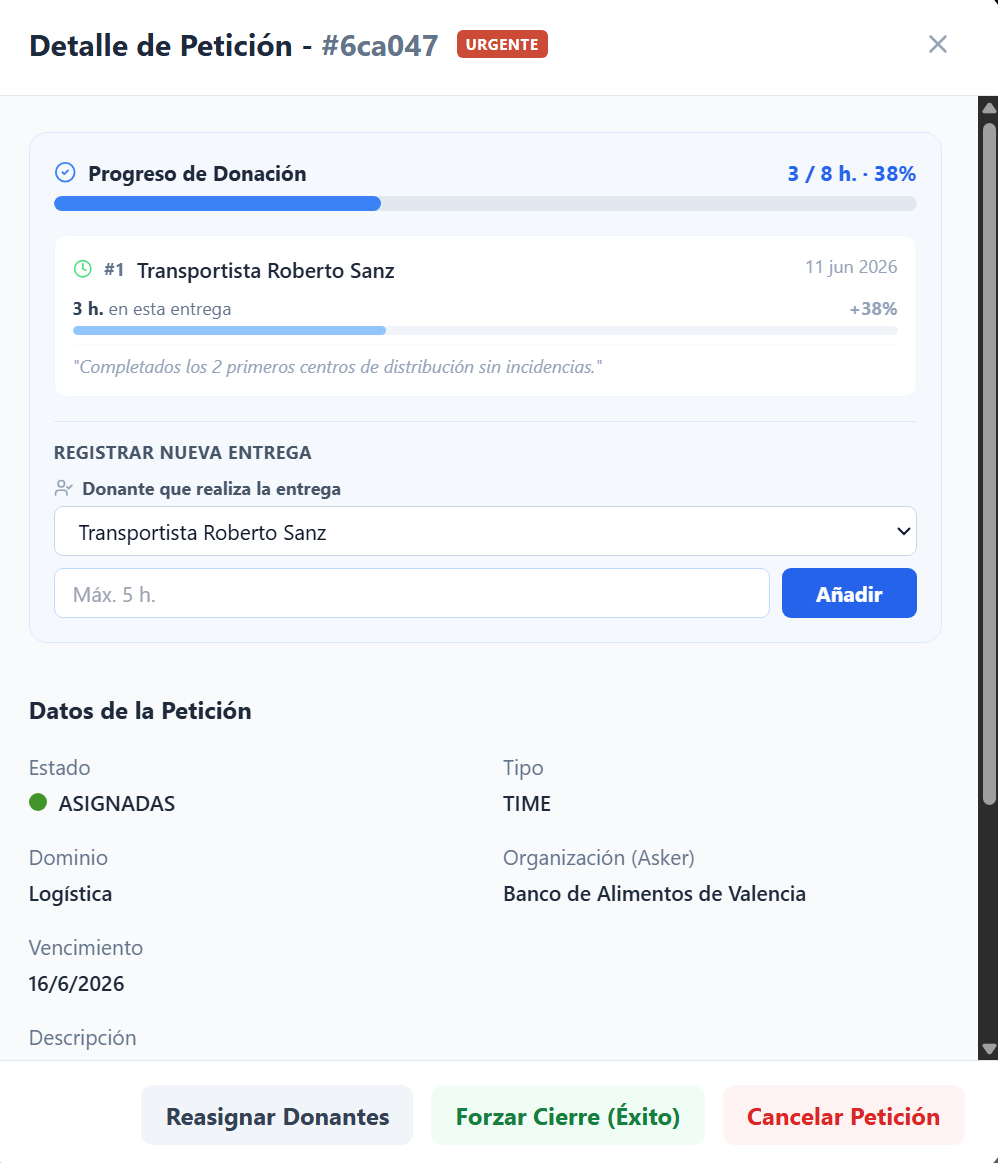
\includegraphics[width=0.72\textwidth]{fulfillment}
\caption[Modal de registro de entrega parcial]{Modal de registro de entrega parcial.}
\label{fig:fulfillment-modal}
\end{figure}

El núcleo de esta lógica reside en el registro de una entrega. Para las peticiones cuantificables —«cosas» y «tiempo»— el servicio suma mediante una agregación en la base de datos todo lo entregado con anterioridad, calcula lo que resta y aplica el control de sobredonación: si la nueva entrega excediese lo pendiente, se rechaza con un 400; si lo iguala exactamente, la petición se da por completada. La creación de la entrega y el eventual cierre de la petición se envuelven en una transacción atómica, de forma que ambos cambios se confirman juntos o no se confirma ninguno, evitando estados inconsistentes ante un fallo intermedio. Las peticiones cualitativas —«conocimiento» y «servicios», que no son fraccionables— se cierran con su primera entrega. El Fragmento~\ref{lst:fulfillment} recoge el corazón de este procedimiento.

\begin{figure}[htbp]
\begin{lstlisting}[caption={Control de sobredonación y cierre automático dentro de una transacción atómica.}, label={lst:fulfillment}]
const previas = await prisma.fulfillment.aggregate({
  where: { askId: data.askId },
  _sum: { quantityDelivered: true }
});
const entregado = previas._sum.quantityDelivered || 0;
const restante  = target - entregado;

if (data.quantityDelivered > restante) {            // control de sobredonacion
  const error = new Error(`Donacion excesiva. Solo faltan ${restante}.`);
  error.statusCode = 400;
  throw error;
}
const isComplete = (data.quantityDelivered === restante);

await prisma.$transaction(async (tx) => {           // atomicidad
  const fulfillment = await tx.fulfillment.create({ data: { /* ... */ } });
  if (isComplete || ask.type === 'EXPERTISE' || ask.type === 'SERVICES') {
    await tx.ask.update({ where: { id: data.askId }, data: { status: 'FULFILLED' } });
  }
  return fulfillment;
});
\end{lstlisting}
\end{figure}

La Figura~\ref{fig:secuencia-fulfillment} representa este recorrido como un diagrama de secuencia, desde que el \textit{Connector} registra la entrega hasta que la petición queda eventualmente cerrada. Junto a este cierre automático, el sistema habilita además un cierre manual anticipado, accesible a los roles gestores —el \textit{Connector}, el \textit{Author} sobre sus propias peticiones y el administrador—, para los casos reales en que la entidad se da por satisfecha con una cobertura parcial; esta acción transita la petición a completada a través del mismo \textit{endpoint} de cambio de estado, bajo confirmación expresa.

\begin{figure}[htbp]
\centering
\resizebox{0.88\textwidth}{!}{%
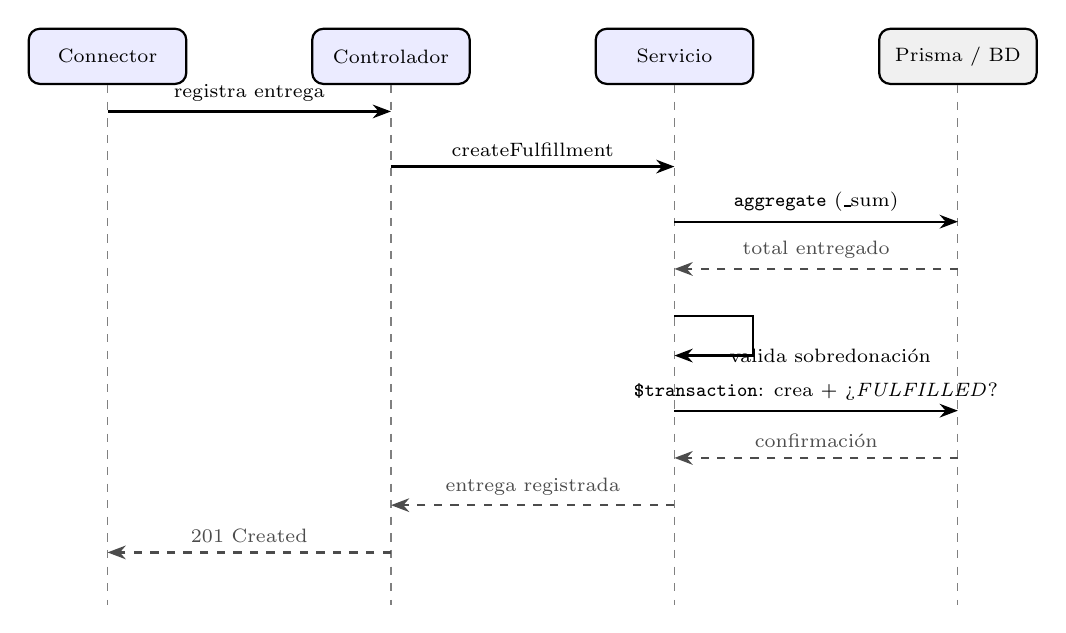
\begin{tikzpicture}[
  font=\scriptsize,
  msg/.style={-{Stealth}, thick},
  ret/.style={-{Stealth}, thick, dashed, gray!60!black},
  actor/.style={rectangle, rounded corners, draw=black, thick, fill=blue!8,
                minimum width=2.0cm, minimum height=0.7cm, align=center},
  store/.style={rectangle, rounded corners, draw=black, thick, fill=gray!12,
                minimum width=2.0cm, minimum height=0.7cm, align=center}
]
  % participantes
  \node[actor] (c)   at (0,0)    {Connector};
  \node[actor] (ctrl) at (3.6,0) {Controlador};
  \node[actor] (svc) at (7.2,0)  {Servicio};
  \node[store] (db)  at (10.8,0) {Prisma / BD};

  % lineas de vida
  \foreach \n in {c,ctrl,svc,db} \draw[gray, dashed] (\n.south) -- ++(0,-6.6);

  % mensajes
  \draw[msg] (0,-0.7)  -- node[above]{registra entrega} (3.6,-0.7);
  \draw[msg] (3.6,-1.4) -- node[above]{createFulfillment} (7.2,-1.4);
  \draw[msg] (7.2,-2.1) -- node[above]{\texttt{aggregate} (\_sum)} (10.8,-2.1);
  \draw[ret] (10.8,-2.7) -- node[above]{total entregado} (7.2,-2.7);

  % autovalidacion
  \draw[msg] (7.2,-3.3) -- ++(1.0,0) -- ++(0,-0.5) -- node[right, xshift=2pt]{valida sobredonación} ++(-1.0,0);

  \draw[msg] (7.2,-4.5) -- node[above]{\texttt{\$transaction}: crea + ¿\textit{FULFILLED}?} (10.8,-4.5);
  \draw[ret] (10.8,-5.1) -- node[above]{confirmación} (7.2,-5.1);
  \draw[ret] (7.2,-5.7) -- node[above]{entrega registrada} (3.6,-5.7);
  \draw[ret] (3.6,-6.3) -- node[above]{201 Created} (0,-6.3);
\end{tikzpicture}%
}
\caption[Secuencia del registro de una entrega parcial]{Secuencia del registro de una entrega parcial.}
\label{fig:secuencia-fulfillment}
\end{figure}

Esta misma relación uno a varios sustenta la republicación de peticiones caducadas. Cuando un autor republica una petición expirada, el sistema no modifica el registro original —que se conserva intacto por trazabilidad— sino que crea una nueva petición; y lo hace calculando el remanente, es decir, restando del objetivo original todo lo que ya se hubiera entregado, de modo que la nueva petición solicita únicamente lo que falta y no duplica la necesidad ya cubierta.

Por último, la transición a \textit{EXPIRED} es la única que ningún actor provoca: la ejecuta un proceso programado. Mediante \textit{node-cron}\footnote{\url{https://github.com/node-cron/node-cron}} se planifica una tarea diaria que, a medianoche, marca como caducadas todas las peticiones abiertas o asignadas cuya fecha límite haya pasado. La operación se resuelve con una única actualización masiva delegada al motor de PostgreSQL, lo que la hace eficiente con independencia del volumen de peticiones afectadas y evita cargar registros en la memoria del servidor. Esta automatización cierra el ciclo de vida descrito en el diseño, garantizando que ninguna petición quede indefinidamente vigente más allá de su plazo.

\chapter{Implantación}

Este capítulo describe la arquitectura objetivo de despliegue, que es consecuencia directa de las decisiones tomadas en el Capítulo~5. En el alcance de este proyecto la plataforma funciona en un entorno local de desarrollo; lo que aquí se expone es cómo debería organizarse un despliegue real, de forma que sirva de referencia para la puesta en marcha definitiva. Al haber diseñado el sistema como una aplicación autónoma con cliente y servidor desacoplados, cada componente puede alojarse en la plataforma más adecuada a su naturaleza sin depender de una infraestructura compartida. La arquitectura objetivo se articula en tres elementos: la base de datos relacional gestionada en la nube, el servidor Node.js con la lógica de negocio y la aplicación React distribuida como archivos estáticos.

\section{Arquitectura en producción}

La Figura~\ref{fig:arquitectura-produccion} describe la topología de despliegue. El navegador del usuario interactúa con dos servicios independientes: descarga la interfaz gráfica como archivos estáticos desde un servicio de distribución de contenidos (CDN) y realiza las llamadas a la API REST contra el servidor Node.js alojado en una plataforma \textit{cloud}. El servidor, a su vez, accede a la base de datos a través de la cadena de conexión gestionada por Supabase\footnote{\url{https://supabase.com/docs}}. Esta separación permite escalar o sustituir cada capa de forma independiente sin afectar a las demás.

\begin{figure}[htbp]
\centering
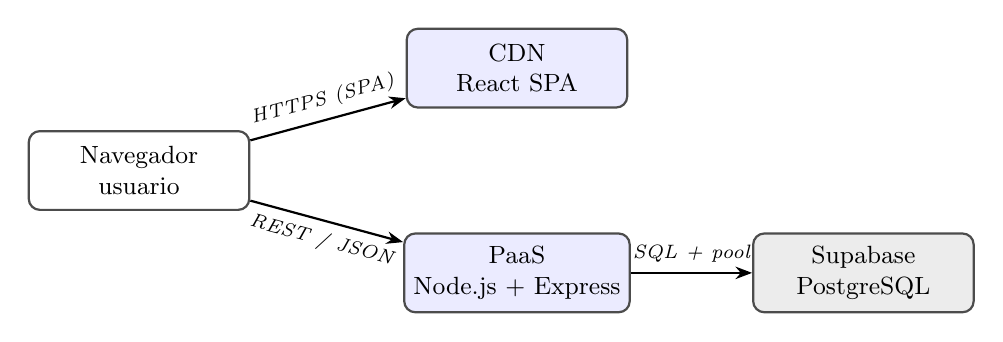
\begin{tikzpicture}[
  comp/.style={rectangle, rounded corners=4pt, draw=black!70, thick, fill=white,
               minimum width=2.8cm, minimum height=1.0cm, align=center, font=\small},
  cloud/.style={rectangle, rounded corners=4pt, draw=black!70, thick, fill=blue!8,
               minimum width=2.8cm, minimum height=1.0cm, align=center, font=\small},
  db/.style={rectangle, rounded corners=4pt, draw=black!70, thick, fill=gray!15,
               minimum width=2.8cm, minimum height=1.0cm, align=center, font=\small},
  arr/.style={-{Stealth[length=6pt]}, thick},
  lbl/.style={font=\scriptsize\itshape}
]
  \node[comp] (browser) at (0,    0)    {Navegador\\usuario};
  \node[cloud] (cdn)    at (4.8,  1.3)  {CDN\\React SPA};
  \node[cloud] (api)    at (4.8, -1.3)  {PaaS\\Node.js + Express};
  \node[db]    (db)     at (9.2, -1.3)  {Supabase\\PostgreSQL};

  \draw[arr] (browser) -- node[lbl, midway, above, sloped]{HTTPS (SPA)} (cdn);
  \draw[arr] (browser) -- node[lbl, midway, below, sloped]{REST / JSON} (api);
  \draw[arr] (api)     -- node[lbl, above]{SQL + \textit{pool}} (db);
\end{tikzpicture}
\caption[Topología de despliegue en producción]{Topología de despliegue en producción.}
\label{fig:arquitectura-produccion}
\end{figure}

\section{Servicio de base de datos}

La base de datos se alojaría en \textit{Supabase}, un servicio gestionado de PostgreSQL que delega en el proveedor la gestión de la infraestructura, reduciendo el riesgo de pérdida de datos frente a una instalación autoalojada (Tabla~\ref{tab:riesgos}). La capa gratuita es suficiente para un entorno de prototipo; un despliegue definitivo requeriría un plan de pago para acceder a recuperación punto a punto y copias de seguridad de mayor granularidad.

El esquema de Prisma declara dos cadenas de conexión con propósitos distintos. La variable \texttt{DATABASE\_URL} apunta al \textit{pooler} de conexiones de Supabase —PgBouncer en modo transacción—, que multiplexa las peticiones de la aplicación sobre un número reducido de conexiones físicas al servidor de base de datos; esto resulta crítico en entornos PaaS donde pueden concurrir múltiples instancias del servidor. La variable \texttt{DIRECT\_URL}, en cambio, establece una conexión directa a PostgreSQL sin intermediario: Prisma la requiere para las operaciones de definición de esquema (DDL), que son incompatibles con el modo transacción del \textit{pooler}. Las migraciones se aplican en producción con el comando \texttt{prisma migrate deploy}, que ejecuta en secuencia únicamente las migraciones pendientes, garantizando la coherencia entre el esquema de la base de datos y el código desplegado.

\section{Despliegue del servidor}

El servidor Node.js necesita una plataforma que mantenga el proceso activo de forma continua. La razón es el servicio de tareas programadas (\texttt{cronService.js}): las arquitecturas sin servidor (\textit{serverless}) no garantizan la continuidad del proceso entre invocaciones y resultan incompatibles con la tarea diaria de caducidad de peticiones. El destino natural para un despliegue definitivo es un servidor dedicado o VPS (\textit{Virtual Private Server}), donde el proceso permanece siempre activo sin limitaciones de inactividad; esta es la opción prevista a largo plazo para \textit{AskingValència}. Para un entorno de validación previo, plataformas gestionadas como \textit{Railway} o \textit{Fly.io} permiten alojar el servidor con proceso persistente, aunque conviene comprobar que la modalidad contratada no suspenda el proceso por inactividad, ya que algunas capas gratuitas lo hacen. El despliegue puede activarse de forma automática mediante un \textit{webhook} al publicar cambios en la rama principal del repositorio de GitHub.

El comando de inicio en producción es \texttt{node server.js}, en lugar del \texttt{nodemon} empleado en desarrollo: la vigilancia de cambios en el sistema de ficheros que ofrece \textit{nodemon} no tiene utilidad en producción y añade una dependencia innecesaria. El servicio \texttt{cronService.js} se inicializa al arrancar el servidor y no requiere configuración adicional; la tarea diaria de caducidad de peticiones queda activa desde el primer momento sin ningún gestor de procesos externo.

La configuración del servidor se lee íntegramente de variables de entorno inyectadas a través del panel de control de la plataforma PaaS. En el entorno de desarrollo local, las mismas variables se cargan desde un fichero \texttt{.env} excluido del control de versiones, de modo que el código no distingue entre ambos entornos.

\section{Despliegue del cliente}

La construcción de producción del cliente se obtiene ejecutando \texttt{npm run build} sobre el proyecto Vite, que compila, miniaturiza y versiona el código React en un conjunto de archivos estáticos alojados en el directorio \texttt{dist/}. Estos archivos no requieren ningún entorno de ejecución del lado del servidor: cualquier CDN o servidor de archivos estático es suficiente para servirlos. Plataformas como \textit{Vercel} o \textit{Netlify} detectan automáticamente proyectos Vite, ejecutan la construcción en cada publicación y distribuyen el resultado desde una red de distribución global.

El único parámetro de configuración del cliente es la URL base de la API REST, inyectada en tiempo de construcción mediante la variable de entorno \texttt{VITE\_API\_URL}. Vite incorpora su valor directamente en el código compilado, de modo que actualizar la URL del servidor solo requiere relanzar la construcción sin modificar ningún fichero de código fuente.

\section{Variables de entorno}

La Tabla~\ref{tab:env-vars} recoge las variables necesarias para operar la plataforma en producción. Su gestión sigue el principio de separación entre configuración y código: ninguna variable se almacena en el repositorio de control de versiones.

\begin{table}[ht]
\centering
\caption[Variables de entorno en producción]{Variables de entorno en producción.}
\label{tab:env-vars}
\footnotesize
\renewcommand{\arraystretch}{1.3}
\begin{tabularx}{\textwidth}{%
  >{\raggedright\arraybackslash}p{3.6cm}%
  >{\raggedright\arraybackslash}p{2.0cm}%
  >{\raggedright\arraybackslash}X}
\toprule
\textbf{Variable} & \textbf{Componente} & \textbf{Descripción} \\
\midrule
\texttt{DATABASE\_URL}    & Backend  & Cadena de conexión con \textit{pooler} (Supabase / PgBouncer) \\
\texttt{DIRECT\_URL}      & Backend  & Conexión directa a PostgreSQL para migraciones de Prisma \\
\texttt{JWT\_SECRET}      & Backend  & Clave de firma de los \textit{tokens} JWT \\
\texttt{GEMINI\_API\_KEY} & Backend  & Clave de acceso a la API de Google Gemini (opcional) \\
\texttt{PORT}             & Backend  & Puerto de escucha del servidor (por defecto, 3000) \\
\texttt{FRONTEND\_URL}    & Backend  & Origen permitido por la política CORS \\
\texttt{VITE\_API\_URL}   & Frontend & URL base de la API REST (inyectada en tiempo de construcción) \\
\bottomrule
\end{tabularx}
\end{table}

La variable \texttt{GEMINI\_API\_KEY} es la única opcional: como se describió en el Capítulo 6, el servicio de generación de Historias de Impacto recurre a una plantilla local cuando la clave no está configurada, lo que permite operar la plataforma en su totalidad sin depender del servicio externo de inteligencia artificial.

\chapter{Pruebas}

La validación del sistema se ha abordado en cuatro fases progresivas. La primera consistió en un análisis estático del código, que detectó problemas de calidad antes de ejecutar ningún flujo. La segunda fue una sesión de validación funcional con \textit{Postman}, en la que se probaron los principales flujos de negocio vinculados a los requisitos funcionales del Capítulo~4 y afloraron varios fallos que se corrigieron antes de dar el sistema por terminado. La tercera verificó la interfaz de usuario navegando manualmente por los flujos en el navegador, donde se detectaron incidencias de internacionalización y usabilidad. La cuarta verificó las restricciones de seguridad y control de acceso correspondientes a los requisitos no funcionales.

\section{Análisis estático del código}

Antes de probar los flujos de negocio, se ejecutó \textit{ESLint} sobre los dos subsistemas del proyecto: el servidor (\texttt{backend/src/}) y el cliente web (\texttt{frontend/src/}). El servidor no disponía de configuración de \textit{linting} previa, por lo que se instaló y configuró \textit{ESLint} con las reglas recomendadas para Node.js. La primera pasada conjunta arrojó \textbf{5 errores y 15 advertencias}, distribuidos según la Tabla~\ref{tab:eslint-primera}.

\begin{table}[ht]
\centering
\caption[Resultados del análisis estático inicial]{Resultados del análisis estático inicial.}
\label{tab:eslint-primera}
\footnotesize
\renewcommand{\arraystretch}{1.3}
\begin{tabularx}{\textwidth}{%
  >{\raggedright\arraybackslash}p{1.0cm}%
  >{\raggedright\arraybackslash}p{1.4cm}%
  >{\raggedright\arraybackslash}p{3.0cm}%
  >{\raggedright\arraybackslash}p{2.8cm}%
  >{\raggedright\arraybackslash}X}
\toprule
\textbf{Tipo} & \textbf{Sist.} & \textbf{Fichero} & \textbf{Regla} & \textbf{Descripción} \\
\midrule
Error & Frontend & \texttt{ConnectorViewAsk\-Modal.jsx} & \texttt{react-hooks} & Subcomponente definido dentro del render; React lo recrea en cada ciclo \\
Error & Frontend & \texttt{Dashboard.jsx} (×2) & \texttt{no-undef} & \texttt{translateDomain} utilizada sin estar definida en el ámbito actual \\
Error & Backend & \texttt{fulfillmentService.js} (×2) & \mbox{\texttt{no-useless-}}\allowbreak\texttt{assignment} & Variables \texttt{totalDeliveredSoFar} y \texttt{remaining} inicializadas a \texttt{0} y sobreescritas antes de ser leídas \\
Aviso & Frontend & Varios & \texttt{no-unused-vars} & Variables y funciones declaradas pero nunca usadas (\texttt{err}, \texttt{getAllAsks}, \texttt{ActiveConnectorListItem}, \texttt{e}) \\
Aviso & Frontend & \texttt{ConfigContext.jsx} & \texttt{react-refresh} & Exporta constantes junto a componentes; interfiere con el HMR \\
Aviso & Frontend & \texttt{LanguageContext.jsx} & \texttt{react-refresh} & Ídem al anterior \\
Aviso & Backend & \texttt{userController.js} (×5) & \texttt{no-unused-vars} & \texttt{passwordHash} desestructurado para excluirlo de la respuesta; el \textit{linter} no reconoce este patrón \\
Aviso & Backend & \texttt{errorHandler.js} & \texttt{no-unused-vars} & Parámetro \texttt{next} requerido por la firma de Express pero no invocado \\
\bottomrule
\end{tabularx}
\end{table}

Los tres errores bloqueantes tenían causas distintas. El de \texttt{ConnectorViewAskModal.jsx} consistía en definir el subcomponente \texttt{GiverSelector} dentro del cuerpo de la función de renderizado: React lo trata como un tipo nuevo en cada ciclo, lo que provoca remontajes innecesarios y puede causar comportamientos inesperados con los \textit{hooks}; la solución fue extraerlo fuera del componente padre. El de \texttt{Dashboard.jsx} era consecuencia de una refactorización incompleta del módulo de internacionalización: la función \texttt{translateDomain} había sido renombrada pero algunas llamadas al nombre anterior quedaron sin actualizar, lo que habría generado un error en tiempo de ejecución al navegar a esa vista. Los dos errores del servidor, en \texttt{fulfillmentService.js}, correspondían a un patrón de inicialización redundante: las variables \texttt{totalDeliveredSoFar} y \texttt{remaining} se declaraban con valor \texttt{0} y se sobreescribían dentro de un bloque condicional sin que el valor inicial llegara a leerse, algo que el compilador permitía pero que el análisis estático señaló como asignación inútil.

Corregidos estos cinco errores y suprimidas las variables huérfanas, la segunda ejecución arrojó \textbf{0 errores}; las advertencias restantes son de carácter no bloqueante —el patrón de desestructuración de \texttt{passwordHash} y los parámetros de firma obligatoria de Express— y no comprometen el funcionamiento del sistema.

\section{Validación funcional con Postman}

Con el servidor en marcha y la base de datos en un estado limpio, se ejecutaron los flujos de negocio principales usando \textit{Postman} para lanzar las llamadas a la API y verificar tanto el cuerpo como el código HTTP de cada respuesta. Las pruebas se organizaron en torno a los requisitos funcionales del Capítulo~4.

\subsection{Primera iteración: fallos detectados}

La primera ronda de pruebas reveló tres problemas que requerían corrección antes de poder validar el sistema.

\textbf{F-01 — Petición creada en estado incorrecto (RF-02, RF-04).} Al crear una petición como \textit{AskAuthor} y consultar inmediatamente su estado, el campo devuelto era \texttt{OPEN} en lugar de \texttt{CREATED}. El efecto práctico era que las peticiones recién creadas saltaban el filtro de aprobación del \textit{Admin} y aparecían directamente en el tablón del \textit{Connector}. La causa era un valor inicial incorrecto en la capa de servicio, que establecía \texttt{status: 'OPEN'} en lugar de \texttt{status: 'CREATED'}. La corrección fue trivial pero el impacto habría sido crítico en producción, pues anulaba por completo el flujo de filtro de calidad previsto en el diseño.

\textbf{F-02 — Sobredonación no controlada (RF-07).} Al registrar un \textit{Fulfillment} con una cantidad mayor que la solicitada, el servidor respondía con HTTP 201 y creaba la entrega sin restricción. El servicio de \textit{Fulfillment} no realizaba ningún cálculo previo del remanente. Se implementó la lógica de agregación con \texttt{prisma.fulfillment.aggregate} para sumar lo ya entregado, calcular lo pendiente y rechazar con HTTP 400 cualquier aportación que lo superase. Junto a esta corrección se añadió el cierre automático de la petición cuando la suma iguala lo solicitado.

\textbf{F-03 — Filtro de visibilidad por rol ausente (RF-12).} Al autenticarse como \textit{AskAuthor} y solicitar el listado de peticiones, la respuesta incluía peticiones de todos los autores del sistema. La función \texttt{getAllAsks} del servicio construía la consulta sin aplicar ningún filtro de propiedad. Se añadió la lógica condicional por rol: el \textit{AskAuthor} recibe solo sus peticiones, el \textit{Connector} recibe las abiertas de su dominio de especialidad más las que gestiona, y el \textit{Giver} únicamente las colaboraciones en las que ha participado.

\subsection{Correcciones aplicadas y segunda iteración}

Tras aplicar las tres correcciones, se repitió la batería de pruebas completa. La Tabla~\ref{tab:pruebas-funcionales} recoge los resultados de esta segunda ejecución, que constituye la validación final del sistema frente a los requisitos funcionales.

\begin{table}[ht]
\centering
\caption[Resultados de la validación funcional final]{Resultados de la validación funcional final.}
\label{tab:pruebas-funcionales}
\footnotesize
\renewcommand{\arraystretch}{1.3}
\begin{tabularx}{\textwidth}{%
  >{\raggedright\arraybackslash}p{0.7cm}%
  >{\raggedright\arraybackslash}p{0.9cm}%
  >{\raggedright\arraybackslash}X%
  >{\raggedright\arraybackslash}p{1.4cm}}
\toprule
\textbf{CP} & \textbf{RF} & \textbf{Flujo validado} & \textbf{Estado} \\
\midrule
CP-01 & RF-02 & El \textit{AskAuthor} crea una petición; la respuesta devuelve \texttt{status: CREATED} & \textbf{Correcto} \\
CP-02 & RF-04 & El \textit{Admin} aprueba la petición; pasa a \texttt{OPEN} y ya es visible para el \textit{Connector} & \textbf{Correcto} \\
CP-03 & RF-05 & El \textit{Connector} vincula dos \textit{Givers}; la petición pasa a \texttt{MATCHED} & \textbf{Correcto} \\
CP-04 & RF-06 & Se registra una entrega parcial (4 de 10 unidades); el estado permanece en \texttt{MATCHED} & \textbf{Correcto} \\
CP-05 & RF-07 & Se registra la entrega restante (6 unidades); el sistema cierra la petición como \texttt{FULFILLED} & \textbf{Correcto} \\
CP-06 & RF-07 & Se intenta registrar una entrega que supera el remanente; el servidor responde HTTP 400 & \textbf{Correcto} \\
CP-07 & RF-09 & El \textit{AskAuthor} republica una petición caducada; se genera una nueva en \texttt{CREATED} con la cantidad pendiente & \textbf{Correcto} \\
CP-08 & RF-10 & El \textit{AskAuthor} genera una Historia de Impacto de una petición \texttt{FULFILLED}; se obtiene el texto & \textbf{Correcto} \\
CP-09 & RF-11 & El \textit{Admin} crea un usuario, lo edita y lo da de baja lógica; no puede autenticarse tras la baja & \textbf{Correcto} \\
CP-10 & RF-12 & Cada rol recibe únicamente las peticiones que le corresponden según su perfil & \textbf{Correcto} \\
CP-11 & RF-13 & El usuario cambia el idioma de la interfaz a valenciano; todos los textos estáticos se actualizan & \textbf{Correcto} \\
\bottomrule
\end{tabularx}
\end{table}

\section{Validación de la interfaz de usuario}

Una vez validada la API con \textit{Postman}, se ejecutó una sesión de pruebas sobre la interfaz gráfica en el navegador, con el cliente React en marcha y conectado al servidor local. El objetivo era verificar los requisitos de usabilidad e internacionalización (RNF-04 y RNF-07) que no quedan cubiertos por las pruebas de API.

\subsection{Primera iteración: fallos detectados}

La navegación manual a través de los flujos principales reveló tres incidencias en la interfaz.

\textbf{UI-01 — Textos sin traducir en el formulario de inicio de sesión (RNF-07).} Al cambiar el idioma a inglés o valenciano, el \textit{placeholder} del campo de correo y el enlace de contraseña olvidada seguían mostrándose en español. La causa era que las claves \texttt{emailPlaceholder} y \texttt{forgotPassword} no estaban definidas en el diccionario de traducciones (\texttt{translations.js}), de modo que el componente usaba cadenas literales en lugar de llamar a la función \texttt{t()}. La corrección consistió en añadir las tres traducciones al diccionario (ES, CAT, EN) y sustituir las cadenas fijas por sus correspondientes llamadas a \texttt{t()}.

\textbf{UI-02 — Botón de selección de idioma ES inaccesible (RNF-04).} Tras cambiar a inglés o valenciano, no era posible volver al español: el botón \texttt{ES} no respondía a los clics. El análisis del DOM reveló que el contenedor del título de la cabecera tenía aplicado el modificador Tailwind \texttt{translate-x-12}, que genera \texttt{transform: translateX(3rem)}. En CSS, \texttt{transform} desplaza tanto el renderizado visual como el área de eventos de puntero, por lo que el contenedor tapaba el botón \texttt{ES} aunque visualmente no se apreciara la superposición. La solución fue reemplazar el desplazamiento por un espaciador invisible de la misma anchura que el grupo de botones, lo que permite que \texttt{justify-between} centre el título sin ningún \texttt{transform}.

\textbf{UI-03 — Truncado de texto en las métricas del panel principal (RNF-04).} En el panel de estadísticas, determinados valores se mostraban cortados con puntos suspensivos en resoluciones de ancho medio. El componente \texttt{MetricCard} aplicaba \texttt{overflow-hidden} y \texttt{truncate} sin reservar espacio suficiente para los valores más largos. Se ajustaron las clases de tamaño para garantizar la legibilidad en el rango de resoluciones objetivo.

\subsection{Correcciones aplicadas y segunda iteración}

Resueltas las tres incidencias, se repitió la navegación manual por los mismos flujos. La Tabla~\ref{tab:pruebas-ui} recoge los resultados de esta segunda iteración.

\begin{table}[ht]
\centering
\caption[Resultados de la validación de interfaz final]{Resultados de la validación de interfaz final.}
\label{tab:pruebas-ui}
\footnotesize
\renewcommand{\arraystretch}{1.3}
\begin{tabularx}{\textwidth}{%
  >{\raggedright\arraybackslash}p{0.7cm}%
  >{\raggedright\arraybackslash}p{0.9cm}%
  >{\raggedright\arraybackslash}X%
  >{\raggedright\arraybackslash}p{1.4cm}}
\toprule
\textbf{CI} & \textbf{RNF} & \textbf{Caso verificado} & \textbf{Estado} \\
\midrule
CI-01 & RNF-07 & Al cambiar el idioma a inglés o valenciano, el \textit{placeholder} del correo y el enlace de contraseña olvidada muestran el texto traducido & \textbf{Correcto} \\
CI-02 & RNF-04 & El selector de idioma responde a los tres botones (ES, CAT, EN) y permite ciclar entre ellos libremente & \textbf{Correcto} \\
CI-03 & RNF-04 & Las métricas del panel principal se muestran sin truncado en las resoluciones objetivo & \textbf{Correcto} \\
CI-04 & RNF-04 & Los flujos principales (crear petición, aprobar, emparejar, entregar) se ejecutan sin errores visuales ni de navegación & \textbf{Correcto} \\
\bottomrule
\end{tabularx}
\end{table}

\section{Pruebas de seguridad y control de acceso}

Esta fase verificó los requisitos no funcionales de seguridad (RNF-01 y RNF-02) enviando de forma deliberada llamadas no autorizadas o malformadas a la API. La Tabla~\ref{tab:pruebas-seguridad} recoge los casos ejecutados y sus resultados, todos correctos en la versión final.

\begin{table}[ht]
\centering
\caption[Resultados de las pruebas de seguridad]{Resultados de las pruebas de seguridad.}
\label{tab:pruebas-seguridad}
\footnotesize
\renewcommand{\arraystretch}{1.3}
\begin{tabularx}{\textwidth}{%
  >{\raggedright\arraybackslash}p{0.7cm}%
  >{\raggedright\arraybackslash}p{1.0cm}%
  >{\raggedright\arraybackslash}X%
  >{\raggedright\arraybackslash}p{1.4cm}}
\toprule
\textbf{CS} & \textbf{RNF} & \textbf{Escenario de prueba} & \textbf{Estado} \\
\midrule
CS-01 & RNF-01 & Llamada a un \textit{endpoint} protegido sin \textit{token}; el servidor responde HTTP 401 & \textbf{Correcto} \\
CS-02 & RNF-01 & Llamada con un \textit{token} manipulado o caducado; el servidor responde HTTP 401 & \textbf{Correcto} \\
CS-03 & RNF-01 & El \textit{AskAuthor} intenta aprobar una petición (acción exclusiva del \textit{Admin}); responde HTTP 403 & \textbf{Correcto} \\
CS-04 & RNF-01 & El \textit{Connector} intenta crear una petición; responde HTTP 403 & \textbf{Correcto} \\
CS-05 & RNF-01 & El \textit{AskAuthor} envía un \texttt{askAuthorId} ajeno en el cuerpo; el servidor lo ignora y usa el del \textit{token} & \textbf{Correcto} \\
CS-06 & RNF-02 & Un usuario con \texttt{isActive: false} intenta iniciar sesión; el servidor responde HTTP 401 & \textbf{Correcto} \\
CS-07 & RNF-03 & Se envía un campo de texto con una sentencia SQL; Prisma lo parametriza y no produce ningún efecto & \textbf{Correcto} \\
\bottomrule
\end{tabularx}
\end{table}

\section{Conclusiones de las pruebas}

El proceso de validación ha confirmado que el sistema cumple los requisitos funcionales, de interfaz y de seguridad definidos en el Capítulo~4. Los fallos detectados en la validación de la API —el estado inicial incorrecto de las peticiones, la ausencia de control de sobredonación y el filtro de visibilidad por rol— afectaban a aspectos centrales de la lógica de negocio y quedaron resueltos antes de finalizar el desarrollo. La validación de la interfaz reveló, además, incidencias de menor gravedad pero de impacto directo en la experiencia del usuario: un bloqueo en el selector de idioma causado por un efecto secundario inesperado de \texttt{transform} sobre los eventos de puntero, y claves de traducción ausentes que dejaban textos sin localizar en el formulario de inicio de sesión. Ambos tipos de hallazgo —los errores de lógica de negocio y los de interfaz— ilustran el valor de combinar la validación de la API con una sesión de navegación manual, ya que ninguna de las dos por sí sola los habría detectado todos.

La principal limitación del enfoque adoptado es la ausencia de pruebas automatizadas. Para una fase de prototipo y un proyecto individual, la validación manual resulta suficiente para demostrar la corrección del sistema; sin embargo, cualquier modificación futura debería apoyarse en una suite de tests que detecte regresiones de forma sistemática.

\chapter{Conclusiones}

\section{Grado de cumplimiento de los objetivos}

El Capítulo 1 formuló seis objetivos específicos que debían materializar la visión general del proyecto. A continuación se evalúa el grado de cumplimiento de cada uno de ellos.

\textbf{Objetivo 1: Analizar el modelo relacional de AskingX.} Cumplido. La revisión de la documentación del proyecto original y las reuniones con el tutor permitieron traducir el modelo a un conjunto de requisitos concretos y a un diagrama de clases que sirvió de base para el desarrollo. El análisis identificó, además, la particularidad más relevante del dominio: el \textit{Asker} no es un usuario del sistema, sino un sujeto gestionado de forma pasiva, lo que reduce su huella de datos y simplifica el modelo de acceso.

\textbf{Objetivo 2: Diseñar e implementar una arquitectura cliente-servidor.} Cumplido. La separación entre el cliente React y el servidor Node.js con Express, organizado en capas de Rutas, Controladores y Servicios, se ha implementado de forma coherente. La arquitectura ha demostrado su valor en la práctica: cuando surgieron cambios de requisitos durante el desarrollo, las modificaciones quedaron circunscritas a la capa de servicios sin afectar a la presentación.

\textbf{Objetivo 3: Modelar la persistencia de datos.} Cumplido. La base de datos PostgreSQL, diseñada y gestionada a través de Prisma ORM, da soporte completo a la trazabilidad de las peticiones y las entregas parciales. La decisión de usar herencia de tabla única para la entidad \textit{Ask} se ha validado en la práctica: las consultas sobre el tablón son simples y no requieren \textit{JOINs} adicionales.

\textbf{Objetivo 4: Garantizar la seguridad y el control de acceso.} Cumplido. La autenticación con JWT, el cifrado de contraseñas con \textit{bcrypt} y los \textit{middlewares} de rol forman un sistema de control de acceso verificado mediante las pruebas descritas en el Capítulo 8. La política de baja lógica preserva la trazabilidad histórica sin exponer datos de ex-empleados en ningún flujo activo.

\textbf{Objetivo 5: Desarrollar el ciclo de vida de las peticiones como una máquina de estados.} Cumplido. La máquina de estados se implementa en la capa de servicio mediante una tabla de transiciones válidas, y la transición automática a \textit{EXPIRED} se garantiza mediante un cron job diario. El control de sobredonación, que cierra la petición de forma atómica cuando se alcanza el objetivo, es la pieza de mayor complejidad y ha funcionado de forma robusta en todas las pruebas.

\textbf{Objetivo 6: Integrar servicios de Inteligencia Artificial.} Cumplido con matices. El módulo de generación de historias funciona correctamente con el modelo \textit{Gemini Flash} y dispone de un mecanismo de respaldo que garantiza su operación incluso sin clave de API. El matiz es que la calidad narrativa del texto generado depende de la riqueza descriptiva de la petición: entradas breves producen historias menos detalladas. La mejora del \textit{prompt} para extraer resultados más elaborados queda como línea de trabajo futuro.

En conjunto, la plataforma cumple los objetivos planteados y ofrece una solución funcional para las necesidades operativas de \textit{AskingValència}. El entregable es una aplicación full-stack desplegable, con autenticación, control de acceso por roles, gestión completa del ciclo de vida de las peticiones y generación asistida de historias de impacto supervisada por el personal de la red.

\section{Relación del trabajo desarrollado con los estudios cursados}

El desarrollo de esta plataforma ha puesto en práctica conocimientos de múltiples áreas del Grado en Ingeniería Informática.

La asignatura de \textit{Gestión de Bases de Datos} proporcionó los fundamentos del modelo relacional que sustentan el diseño del esquema: la integridad referencial, las relaciones de uno a muchos y de muchos a muchos y la normalización del modelo. La aplicación de herencia de tabla única para la entidad \textit{Ask} es un ejemplo directo de las técnicas de persistencia trabajadas en ese contexto, aplicadas aquí a un dominio real con requisitos de trazabilidad parcial.

La asignatura \textit{PIN} orientó directamente la organización del proyecto. La estructuración en \textit{Sprints} temáticos y las revisiones periódicas con el tutor como punto de validación son aplicaciones de la metodología ágil estudiada en esa asignatura. La adaptación al contexto de un proyecto individual —sin ceremonias formales de Scrum pero con la misma disciplina iterativa— es en sí misma un ejercicio de criterio sobre cuándo y cómo aplicar una metodología.

La asignatura de \textit{Integración e Interoperabilidad} (IEI) está presente en el núcleo de la arquitectura. El diseño de la API REST como contrato entre cliente y servidor —recursos identificados por URI, métodos HTTP semánticos e intercambio de datos en JSON— es la aplicación directa de los principios de integración estudiados. Prisma ORM actúa además como capa de traducción entre el modelo de objetos de la aplicación y el esquema relacional de PostgreSQL, y la conexión con la API externa de Gemini añade una tercera frontera de interoperabilidad que requirió gestionar autenticación, formato de petición y comportamiento ante fallos de un servicio de terceros.

El área de seguridad e identidad digital está presente en varias capas del sistema. La autenticación mediante JWT, el cifrado de contraseñas con \textit{bcrypt}, la política RBAC y el mecanismo \textit{anti-spoofing} son aplicaciones de los principios de autenticación y autorización trabajados en las asignaturas de seguridad de la rama.

El desarrollo del cliente web consolidó conocimientos del área de desarrollo de interfaces y aplicaciones web: el modelo de componentes de React, la programación asíncrona con la API \textit{Fetch} y la gestión del estado en una aplicación de página única. El enfoque \textit{mobile-first} y el uso de \textit{Tailwind CSS} conectan con los principios de usabilidad y diseño de interfaces estudiados a lo largo del grado.

La especificación de requisitos funcionales y no funcionales, el modelado conceptual del dominio y la elaboración del análisis de riesgos ponen en práctica las técnicas de análisis y diseño de sistemas aprendidas en las asignaturas de ingeniería del software de la titulación, aplicadas aquí a un dominio real con restricciones éticas y legales concretas.

La asignatura de \textit{Mantenimiento y Evolución del Software} (MES) tiene su reflejo directo en el Capítulo~8. El proceso de validación adoptado —análisis estático con \textit{ESLint}, pruebas funcionales con \textit{Postman} organizadas en dos iteraciones, validación manual de la interfaz y verificación del control de acceso— reproduce el ciclo de detección y corrección de defectos estudiado en esa asignatura. Los tres fallos de lógica de negocio descubiertos en la primera iteración de \textit{Postman} (estado inicial incorrecto, ausencia de control de sobredonación y filtro de visibilidad por rol) ilustran además por qué las pruebas deben ejecutarse antes de dar el sistema por terminado, y no como trámite final. La deuda técnica más evidente que queda abierta —la ausencia de una suite de tests automatizados— conecta directamente con los principios de mantenibilidad y prevención de regresiones que vertebran la asignatura.

Por último, la integración de un modelo de lenguaje externo y el análisis de sus implicaciones bajo el Reglamento Europeo de IA abre una dimensión que no estaba contemplada en el plan de estudios cuando se cursó, lo que refleja la velocidad a la que evoluciona el sector y la necesidad de que el perfil del ingeniero se adapte continuamente a ese ritmo.

Más allá de los conocimientos técnicos, el trabajo ha exigido poner en práctica varias competencias transversales del título. El \textbf{análisis y resolución de problemas} y el \textbf{pensamiento crítico} se han ejercitado al evaluar alternativas de diseño y depurar la lógica de negocio. La competencia de \textbf{diseño y proyecto} se refleja en la conducción del trabajo desde el análisis de requisitos hasta la validación. El \textbf{aprendizaje permanente} ha sido constante, al haber tenido que asimilar de forma autónoma tecnologías no vistas en el aula. Y la \textbf{comunicación efectiva} se concreta en la redacción de esta memoria y en la preparación de su defensa.

\chapter{Trabajos futuros}

La versión actual cubre el ciclo de vida completo de las peticiones y ofrece una base sólida para el funcionamiento de \textit{AskingValència}. No obstante, el análisis del proyecto y la experiencia acumulada durante el desarrollo apuntan a varias líneas de evolución que aumentarían el valor del sistema.

\textbf{Pruebas automatizadas.} La ausencia de una suite de tests automatizados es la deuda técnica más evidente del proyecto. Implementar pruebas de integración para los \textit{endpoints} críticos —el ciclo de vida de la petición, el control de sobredonación y el filtrado por rol— reduciría el riesgo de regresiones a medida que el sistema crezca.

\textbf{Mejora del módulo de IA.} La calidad de las historias generadas depende de la riqueza del \textit{prompt}. Un trabajo de ingeniería de \textit{prompts} orientado a obtener narrativas más detalladas, junto con la anonimización sistemática de los datos enviados al modelo, mejoraría tanto la calidad del texto como la privacidad de los datos tratados.

\textbf{Aplicación móvil nativa.} Una aplicación móvil dirigida a los facilitadores facilitaría el trabajo de campo, donde la mayor parte de las interacciones con entidades y donantes ocurre fuera de la oficina. La API REST diseñada es compatible con cualquier cliente nativo sin necesidad de modificar el servidor.

\textbf{Despliegue en producción.} La plataforma funciona actualmente en un entorno local de desarrollo. El siguiente paso natural es su puesta en marcha en un servidor dedicado siguiendo la arquitectura objetivo descrita en el Capítulo~7: base de datos en \textit{Supabase}, servidor Node.js con proceso persistente en un VPS y cliente React distribuido desde un CDN. Este despliegue convertiría la solución en una herramienta operativa real para \textit{AskingValència}, permitiendo que el equipo de facilitadores acceda a la plataforma desde cualquier dispositivo sin depender de un entorno local.

\textbf{Expansión a otras AskingCities.} El diseño \textit{standalone} del sistema permite desplegarlo como una instancia independiente en cada ciudad. La siguiente evolución natural sería un modelo \textit{multi-tenant}, en el que una sola instalación sirva a varias ciudades de la red con datos completamente aislados entre sí. Esta línea transformaría la plataforma en una infraestructura compartida para el movimiento AskingX en su conjunto.

\bibliographystyle{ieeetr}
\bibliography{bibliografia}

\cleardoublepage

\chapter{Anexos}
\section{Glosario de términos}

A continuación se recogen los principales términos técnicos empleados a lo largo de la memoria, con una breve definición orientada al contexto del proyecto.

\begin{description}
  \item[API REST] Estilo arquitectónico para diseñar servicios web sin estado y orientados a recursos, sobre HTTP. La comunicación entre el cliente y el servidor de la plataforma sigue este estilo, intercambiando datos en formato JSON.
  \item[Anti-spoofing] Conjunto de medidas que impiden la suplantación de identidad. En el sistema, la autoría de una petición se toma siempre del \textit{token} de sesión y nunca de los datos enviados por el cliente.
  \item[Baja lógica (\textit{soft-delete})] Técnica que marca un registro como inactivo en lugar de borrarlo físicamente, preservando la trazabilidad histórica. Se aplica a la eliminación de usuarios.
  \item[bcrypt] Función de derivación de claves usada para cifrar contraseñas de forma unidireccional, con un factor de coste configurable que la hace resistente a ataques de fuerza bruta.
  \item[Cron] Mecanismo de planificación de tareas que se ejecutan de forma periódica y automática. El sistema lo emplea para caducar peticiones vencidas a diario.
  \item[CORS (\textit{Cross-Origin Resource Sharing})] Mecanismo de seguridad del navegador que controla qué orígenes externos pueden hacer peticiones a una API. El servidor declara el origen del cliente como permitido para que las llamadas desde el frontend no sean bloqueadas.
  \item[CDN (\textit{Content Delivery Network})] Red de distribución de contenidos: conjunto de servidores distribuidos geográficamente que sirven archivos estáticos (HTML, CSS, JavaScript) desde el punto más cercano al usuario. Se emplea para distribuir la aplicación React en producción.
  \item[CRUD] Acrónimo de las cuatro operaciones básicas sobre datos: crear, leer, actualizar y borrar (\textit{Create, Read, Update, Delete}).
  \item[Drag and Drop] Interacción de «arrastrar y soltar» elementos de la interfaz. El tablero del \textit{Connector} la usa para mover peticiones entre columnas.
  \item[DTO (\textit{Data Transfer Object})] Objeto que transporta datos entre capas o sistemas. En el servidor, los DTO de entrada se validan con \textit{Zod} antes de alcanzar la lógica de negocio.
  \item[Endpoint] Punto de entrada de la API, identificado por un método HTTP y una ruta, que expone una operación concreta del sistema.
  \item[Fallback (respaldo)] Comportamiento alternativo que entra en acción cuando la vía principal falla. La generación de historias recurre a una plantilla local si el servicio de IA no está disponible.
  \item[Filtrado a nivel de consulta] Técnica que restringe los datos que un usuario puede ver aplicando el filtro directamente en el acceso a la base de datos, en lugar de descartarlos después en la presentación.
  \item[Herencia de tabla única (\textit{Single-Table Inheritance})] Patrón de persistencia que almacena varios subtipos de una entidad en una sola tabla, distinguiéndolos por un atributo de tipo. Se aplica a la petición (\textit{Ask}).
  \item[HMR (\textit{Hot Module Replacement})] Recarga de módulos en caliente: actualiza el código de la aplicación en el navegador sin recargar la página entera, acelerando el desarrollo.
  \item[HTTP / JSON] Protocolo de transferencia de la web (HTTP) y formato ligero de intercambio de datos (JSON) sobre el que se comunican cliente y servidor.
  \item[Human-in-the-loop] Patrón en el que una persona supervisa y confirma una acción antes de que tenga efecto. Se aplica a la confirmación de entregas y a la publicación de historias generadas por IA.
  \item[JWT (\textit{JSON Web Token})] Token firmado que acredita la identidad y el rol de un usuario, permitiendo una autenticación sin estado en el servidor.
  \item[Kanban] Método visual de gestión que organiza el trabajo en columnas por estado. Da forma al tablero del \textit{Connector}.
  \item[LLM (\textit{Large Language Model})] Modelo de lenguaje de gran tamaño capaz de generar texto. El sistema lo utiliza para redactar las Historias de Impacto.
  \item[Middleware] Componente que intercepta una petición HTTP entre su recepción y su procesamiento. Se emplea para la autenticación, el control de acceso por rol y el tratamiento de errores.
  \item[Multi-tenant] Arquitectura en la que una sola instalación del software sirve a varios clientes (inquilinos) con sus datos completamente aislados entre sí. Se plantea como evolución futura para dar servicio a varias ciudades de la red AskingX desde una misma plataforma.
  \item[Mobile-first] Enfoque de diseño de interfaces que prioriza la experiencia en dispositivos móviles y la amplía después a pantallas mayores.
  \item[ORM (\textit{Object-Relational Mapping})] Capa que traduce entre los objetos del código y las tablas de una base de datos relacional. El proyecto usa \textit{Prisma} como ORM.
  \item[PaaS (\textit{Platform as a Service})] Modelo de servicio en la nube que proporciona una plataforma gestionada para desplegar aplicaciones sin gestionar el sistema operativo ni la infraestructura subyacente. Se usa en el capítulo de implantación para alojar el servidor Node.js.
  \item[RBAC (\textit{Role-Based Access Control})] Control de acceso basado en roles: cada usuario opera únicamente dentro de las competencias asociadas a su rol.
  \item[SPA (\textit{Single Page Application})] Aplicación web de página única que actualiza la vista sin recargar el documento completo, intercambiando solo datos con el servidor.
  \item[Transacción atómica] Conjunto de operaciones de base de datos que se confirman todas juntas o ninguna, evitando estados intermedios inconsistentes. Envuelve el registro de una entrega y el posible cierre de la petición.
  \item[Upsert] Operación que inserta un registro si no existe o lo actualiza si ya existe. Garantiza la relación uno a uno entre una petición y su historia.
  \item[VPS (\textit{Virtual Private Server})] Servidor virtual privado: máquina virtual alojada en infraestructura compartida que se comporta como un servidor dedicado, con proceso siempre activo y sin limitaciones de inactividad. Es el destino de despliegue previsto a largo plazo para el servidor Node.js de \textit{AskingValència}.
  \item[Webhook] Mecanismo de notificación HTTP mediante el cual un servicio externo (como GitHub) llama automáticamente a una URL configurada cuando ocurre un evento. Se emplea para activar el despliegue del servidor cada vez que se publican cambios en la rama principal del repositorio.
\end{description}

\cleardoublepage

%%%%%%%%%%%%%%%%%%%%%%%%%%%%%%%%%%%%%%%%%%%%%%%%%%%%%%%%%%%%%%%%%%%%%%%%%%%%%%%
%                            APÉNDICES (¡Si los hay!)                         %
%%%%%%%%%%%%%%%%%%%%%%%%%%%%%%%%%%%%%%%%%%%%%%%%%%%%%%%%%%%%%%%%%%%%%%%%%%%%%%%

\appendix

%%%%%%%%%%%%%%%%%%%%%%%%%%%%%%%%%%%%%%%%%%%%%%%%%%%%%%%%%%%%%%%%%%%%%%%%%%%%%%%
%   APÉNDICES (opcionales). Añade aquí, si los necesitas, un manual de        %
%   instalación, el listado de endpoints de la API, etc. con \chapter{...}    %
%%%%%%%%%%%%%%%%%%%%%%%%%%%%%%%%%%%%%%%%%%%%%%%%%%%%%%%%%%%%%%%%%%%%%%%%%%%%%%%

\chapter{Alineación con los Objetivos de Desarrollo Sostenible (ODS)}
\label{ap:ods}

Más allá de su finalidad técnica, \textit{AskingValència} es, por naturaleza, una herramienta de acción social, y como tal se inscribe en el marco de la Agenda 2030 de Naciones Unidas. Este apéndice analiza qué Objetivos de Desarrollo Sostenible (ODS) atiende la solución y, sobre todo, en qué hechos concretos del sistema se sustenta cada uno, evitando atribuirse metas que el proyecto no pueda respaldar.

De los 17 ODS, el trabajo guarda una relación alta con tres —el 10, el 11 y el 17—, que constituyen la razón de ser del modelo, y una relación media con el ODS 4, condicionada al tipo de necesidad que se canalice en cada petición. La Tabla~\ref{tab:ods} recoge esta valoración para el conjunto de los diecisiete objetivos.

\begin{table}[ht]
\centering
\caption[Relación del trabajo con los ODS]{Grado de relación del trabajo con los Objetivos de Desarrollo Sostenible.}
\label{tab:ods}
\footnotesize
\renewcommand{\arraystretch}{1.25}
\begin{tabularx}{\textwidth}{%
  >{\raggedright\arraybackslash}X%
  >{\centering\arraybackslash}p{1.2cm}%
  >{\centering\arraybackslash}p{1.2cm}%
  >{\centering\arraybackslash}p{1.2cm}%
  >{\centering\arraybackslash}p{1.6cm}}
\toprule
\textbf{Objetivo de Desarrollo Sostenible} & \textbf{Alto} & \textbf{Medio} & \textbf{Bajo} & \textbf{No Procede} \\
\midrule
Fin de la pobreza                          &            &            &  & \ding{51} \\
Hambre cero                                &            &            &  & \ding{51} \\
Salud y bienestar                          &            &            &  & \ding{51} \\
Educación de calidad                       &            & \ding{51}  &  &           \\
Igualdad de género                         &            &            &  & \ding{51} \\
Agua limpia y saneamiento                  &            &            &  & \ding{51} \\
Energía asequible y no contaminante        &            &            &  & \ding{51} \\
Trabajo decente y crecimiento económico    &            &            &  & \ding{51} \\
Industria, innovación e infraestructuras   &            &            &  & \ding{51} \\
Reducción de las desigualdades             & \ding{51}  &            &  &           \\
Ciudades y comunidades sostenibles         & \ding{51}  &            &  &           \\
Producción y consumo responsables          &            &            &  & \ding{51} \\
Acción por el clima                        &            &            &  & \ding{51} \\
Vida submarina                             &            &            &  & \ding{51} \\
Vida de ecosistemas terrestres             &            &            &  & \ding{51} \\
Paz, justicia e instituciones sólidas      &            &            &  & \ding{51} \\
Alianzas para lograr objetivos             & \ding{51}  &            &  &           \\
\bottomrule
\end{tabularx}
\end{table}

\section{Justificación del cumplimiento}

\subsection{Relación alta}

\textbf{ODS 10 — Reducción de las Desigualdades.} Es el objetivo más directamente vinculado al proyecto. El propósito de la plataforma es redistribuir recursos que ya existen en la ciudad, pero que no encuentran el camino hasta quien los necesita, hacia entidades y personas en situación de vulnerabilidad. Esto incide de lleno en la meta 10.2 (promover la inclusión social y económica de todas las personas). El compromiso no se queda en la intención: se traslada a decisiones de diseño concretas. El hecho de que el \textit{Asker} no disponga de cuenta minimiza la huella de datos de los colectivos más expuestos; la política RBAC y el filtrado a nivel de consulta protegen su información; y la trazabilidad atómica de cada \textit{Fulfillment} hace que la redistribución de recursos sea auditable y no un mero gesto declarativo.

\textbf{ODS 11 — Ciudades y Comunidades Sostenibles.} El modelo AskingX nace de una idea profundamente urbana: las ciudades ya disponen de los recursos que necesitan y solo les falta un mecanismo ágil para movilizarlos. La plataforma activa esa «superconectividad» local, conectando capacidades latentes con necesidades comunitarias, en línea con la meta 11.3 (urbanización inclusiva y participativa). Su diseño \textit{standalone} y replicable está pensado expresamente para extenderse a otras \textit{AskingCities}, lo que refuerza redes de resiliencia comunitaria más allá de una única ciudad. Las Historias de Impacto, por su parte, alimentan la cohesión social y la cultura de ayuda mutua que sostiene el ecosistema.

\textbf{ODS 17 — Alianzas para lograr los Objetivos.} La plataforma es, en esencia, un generador de alianzas. Su función es tejer colaboraciones entre actores que de otro modo no se encontrarían: entidades del tercer sector, donantes particulares, expertos e instituciones. Esto responde a las metas 17.16 y 17.17, centradas en las alianzas multiactor. El rol del \textit{Connector} y el mecanismo de emparejamiento formalizan esas alianzas, mientras que la trazabilidad y los cuadros de mando aportan la rendición de cuentas que cualquier colaboración sólida necesita para mantenerse en el tiempo.

\subsection{Relación media}

\textbf{ODS 4 — Educación de Calidad.} Entre las entidades atendidas figuran centros educativos, y el sistema contempla peticiones de conocimiento (\textit{EXPERTISE}) y de dedicación de tiempo (\textit{TIME}) que pueden materializarse en mentorías, formación o apoyo escolar. La clasificación de las peticiones por dominios temáticos permite dirigir esa experiencia educativa hacia donde resulta más necesaria, contribuyendo a la meta 4.5 (eliminar las disparidades en el acceso a la educación). Se trata de una relación condicionada al tipo de ayuda que se gestione en cada momento.

%%%%%%%%%%%%%%%%%%%%%%%%%%%%%%%%%%%%%%%%%%%%%%%%%%%%%%%%%%%%%%%%%%%%%%%%%%%%%%%
%                              FI DEL DOCUMENT                                %
%%%%%%%%%%%%%%%%%%%%%%%%%%%%%%%%%%%%%%%%%%%%%%%%%%%%%%%%%%%%%%%%%%%%%%%%%%%%%%%

\end{document}
